%%%%%%%%%%%%%%%%%%%%%%%%%%%%%%%%%%%%%%%%%%%%%%%%%%%%%%%%%%%%%%%
%%%  Glassines in one dimensional hopping model
%%%%%%%%%%%%%%%%%%%%%%%%%%%%%%%%%%%%%%%%%%%%%%%%%%%%%%%%%%%%%%%

\documentclass[onecolumn,fleqn]{revtex4}
%\documentclass[twocolumns,fleqn,aps,pra,floats,floatfix]{revtex4}
%\documentclass[aps,pra,floats,floatfix]{revtex4-1}
%\documentclass[aps,pra,floats,floatfix,twocolumn]{revtex4}

\def \thebibliography#1{
\noindent {\bf References:}
\list
{\relax}{
\setlength{\labelsep}{2mm}
\setlength{\itemindent}{0mm}
\setlength{\leftmargin}{6mm}
\setlength{\itemsep}{-0.3mm}
}
\def\newblock{\hskip .11em plus .33em minus .07em}
\sloppy\clubpenalty4000\widowpenalty4000\sfcode`\.=1000\relax}

% special 
\usepackage{ifthen}
\usepackage{ifpdf}
\usepackage{color}
%
%\ifpdf
%\usepackage{graphicx}
%\usepackage{epstopdf}
%\else
\usepackage{graphicx}
\usepackage{epsfig}
%\fi
\graphicspath{{/Users/danielhurowitz/PROJ/NHR/Figs/}{/Users/danielhurowitz/PROJ/NEG/Figs/}{./}}

\usepackage[pdftitle={},bookmarks]{hyperref}


% fonts
\usepackage{latexsym}
\usepackage{amsmath}
\usepackage{amssymb}
\usepackage{bm}
\usepackage{wasysym}

%\usepackage{hyperref}

%%%%%%%%%%%%%%%%%%%%%%%%%%%%%%%%%%%%%%%%%%%%%%%%%%%%%%%%%%%%%%%%

% NEW 
\newcommand{\abs}[1]{\left|#1\right|}
\newcommand{\Prob}{\mbox{Prob}\,}
\newcommand{\erf}{\mbox{erf}\,}

% math symbols I
\newcommand{\sinc}{\mbox{sinc}}
\newcommand{\const}{\mbox{const}}
\newcommand{\trc}{\mbox{trace}}
\newcommand{\intt}{\int\!\!\!\!\int }
\newcommand{\ointt}{\int\!\!\!\!\int\!\!\!\!\!\circ\ }
\newcommand{\ar}{\mathsf r}
\newcommand{\im}{\mbox{Im}}
\newcommand{\re}{\mbox{Re}}

% math symbols II
\newcommand{\eexp}{\mbox{e}^}
\newcommand{\bra}{\left\langle}
\newcommand{\ket}{\right\rangle}

% Mass symbol
\newcommand{\mass}{\mathsf{m}} 
\newcommand{\Mass}{\mathsf{M}} 

% more math commands
\newcommand{\tbox}[1]{\mbox{\tiny #1}}
\newcommand{\bmsf}[1]{\bm{\mathsf{#1}}} 
%\newcommand{\amatrix}[1]{\matrix{#1}} 
\newcommand{\amatrix}[1]{\begin{matrix} #1 \end{matrix}} 
\newcommand{\pd}[2]{\frac{\partial #1}{\partial #2}}

% equations
\newcommand{\mylabel}[1] {\textcolor{blue}{[#1]}\label{#1}} %{\label{#1}}
%\newcommand{\mylabel}[1]{\label{#1}}  %{\textcolor{blue}{[#1]}\label{#1}}

%\newcommand{\mylabel}[1] {} %{\label{#1}}
\newcommand{\beq}{\begin{eqnarray}}
\newcommand{\eeq}{\end{eqnarray}} 
\newcommand{\be}[1]{\begin{eqnarray}\ifthenelse{#1=-1}{\nonumber}{\ifthenelse{#1=0}{}{\mylabel{e#1}}}}
\newcommand{\ee}{\end{eqnarray}} 

% arrangement
\newcommand{\drawline}{\begin{picture}(500,1)\line(1,0){500}\end{picture}}
\newcommand{\bitem}{$\bullet$ \ \ \ }
\newcommand{\Cn}[1]{\begin{center} #1 \end{center}}
\newcommand{\mpg}[2][1.0\hsize]{\begin{minipage}[b]{#1}{#2}\end{minipage}}
\newcommand{\mpgt}[2][1.0\hsize]{\begin{minipage}[t]{#1}{#2}\end{minipage}}
\newcommand{\putgraph}[2][width=0.30\hsize]{\includegraphics[#1]{#2}}

% more
\newcommand{\Eq}[1]{\textcolor{blue}{equation~(\ref{#1})}} %{equation~(\ref{#1})}
\newcommand{\Fig}[1] {\textcolor{blue}{Fig.~\ref{#1}}} %{Fig.~\ref{#1}}
\newcommand{\hide}[1]{\textcolor{red}{[hidden text]}} %{}
\newcommand{\rmrk}[1]{\textcolor{red}{#1}}
%\newcommand{\Rmrk}[1]{\textcolor{blue}{\LARGE\bf #1}}


%\renewcommand{\includegraphics}[2][]{}
\renewcommand{\cite}[1]{\textcolor{blue}{[\onlinecite{#1}}]} %{[\onlinecite{#1}]} 


\def\circbul{{\bigcirc \mkern-8mu _{\bullet} \mkern-8mu}} 


\newcommand{\ola}{\protect\overleftarrow}
\newcommand{\ora}{\protect\overrightarrow}

% Page setup
\setlength{\parindent}{0cm} 
\setlength{\parskip}{0.3cm} 

%counters
\renewcommand{\thesection}{\arabic{section}}
\renewcommand{\thesubsection}{\arabic{subsection}}
\setcounter{section}{0}
\setcounter{subsection}{0}

% Sections
\newcommand{\sect}[1]
{
\addtocounter{section}{1} 
\setcounter{subsection}{0}
\ \\ 
\pdfbookmark[2]{\thesection. \ #1}{sect.\thesection}
{\Large\bf $=\!=\!=\!=\!=\!=\;$ [\thesection] \ #1}  
\nopagebreak
}

% subections
\newcommand{\subsect}[1]
{
\addtocounter{subsection}{1} 
\ \\ 
\pdfbookmark[2]{\ \ \ \ \thesection.\thesubsection. \ #1}{subsect.\thesection.\thesubsection}
{\bf $=\!=\!=\!=\!=\!=\;$ [\thesection.\thesubsection] \ #1}  
\nopagebreak
}

%%%%%%%%%%%%%%%%%%%%%%%%%%%%%%%%%%%%%%%%%%%%%%%%%%%%%%%%%%%%%%%%%%%%%%%%%%%%%%%%%%%%%%%%%%
%%%%%%%%%%%%%%%%%%%%%%%%%%%%%%%%%%%%%%%%%%%%%%%%%%%%%%%%%%%%%%%%%%%%%%%%%%%%%%%%%%%%%%%%%%
 
\begin{document}

\title{One dimensional hopping model - interplay of resistor-network and Sinai spreading}

\author{Notes by Daniel Hurowitz}

\affiliation{
Department of Physics, Ben-Gurion University of the Negev, P.O.B. 653, Beer-Sheva 84105, Israel
}
\maketitle


%%%%%%%%%%%%%%%%%%%%%%%%%
\sect{Introduction}

The conventional view of variable-range-hopping is based on the assumption 
that the rates of transitions are {\em symmetric} 
but have log-wide distribution as in glassy systems. 
Namely, the rate at the $n$th bond is written as 
%
\beq 
g_n \ \ = \ \ \text{rate of transition} \ \ = \ \ \exp(-\mathcal{B}_n)
\eeq
% 
where the barriers $\mathcal{B}_n$ have (say) a box distribution.
Consequently a resistor-network analysis is most appropriate for the 
analysis,leading to an Ohmic result for the current, namely $I\propto 1/L$,  
where $L$ is the length of the sample, but the prefactor is exponentially small. 

Contrary to that Sinai has considered a model where the rates are {\em asymmetric}. 
The asymmetry of transitions in the $n$th bond is characterized by   
%
\beq
\mathcal{E}_n \ \ = \ \ \ln\left( \frac{\ora{w}_{n}}{\ola{w}_{n}} \right)  
\eeq
%  
which we call ``stochastic field". 
At equilibrium $\mathcal{E}_n = (E_{n}-E_{n+1})/T$, 
where $T$ is the temperature.  
More generally we can define a stochastic potential 
%
\beq
V_n \ \ = \ \ \sum_{n'=0}^n \mathcal{E}_{n'}
\eeq
% 
In non-equilibrium circumstances the telescopic correlations are likely 
to be broken, the sum becomes of order $\sqrt{L}$,   
and therefore $I\propto \exp(-\sqrt{L})$ due to this buildup 
of an activation barrier. 
    

%%%%%%%%%%%%%%%%%%%%%%%%%
\sect{The model, and main observations}

Below we consider a 1D model were we have an interplay of resistor-network physics 
(due to random couplings) and Sinai physics (due to random stochastic field).       
Specifically we consider an $N$ site ring with near-neighbor transitions.
Each bond is characterized by two numbers:
%
\be{1}
\mathcal{B}_n \ \ &=& \ \ \text{barriers} \ \ = \ \ \text{random} \in [-\Delta,\Delta] \\
\mathcal{E}_n \ \ &=& \ \ \text{stochastic field} \ \ = \ \ \text{random} \in [s-\sigma,s+\sigma] 
\ee
%
Accordingly the transition rates across the $n^{th}$ bond are 
%
\be{1}
\ora{w}_{n} &=&  w_{n+1,n} \ = \ g_n \eexp{ \mathcal{E}_n/2} \ = \ \eexp{-\mathcal{B}_n + \mathcal{E}_n/2} \\
\ola{w}_{n} &=&  w_{n,n+1} \ = \ g_n \eexp{-\mathcal{E}_n/2} \ = \ \eexp{-\mathcal{B}_n - \mathcal{E}_n/2}
\ee
%
The average stochastic field~$s$ is called in the literature ``affinity". 
It can be written as $s=\text{Force}/T$, where the force 
is defined as the slope of the potential, and $T$ is the temperature.
The term ``slope" is appropriate if we view our model as describing 
a periodic lattice with $N$-site unit cell. But we prefer to have in 
mind a ring geometry so the more appropriate notion is ``stochastic motive force":
%
\beq
S_{\circlearrowleft} \ \ = \ \ \sum_{n\in\text{ring}}^N \mathcal{E}_{n} \ \ = \ \ Ns
\eeq  
\clearpage
%%%%%%%%%%%%%%%%%%%%%%%%%%%%%%%%%%%%%
%%%%%%%%%%%%%%%%%%%%%%%%%%%%%%%%%%%%%%%

%%%%%%%%%%%%%%%%%%%%%%%%%%
%%%%%%%%%%%%%%%%%%%%%%%%%%%%%%%%%%%%%%%%


% complex gap , this is done by looking at how the 
%real part of the complex eigenvalues behave as $\mathcal{S}$ increases.
%Adding an imaginary part, such that $x\to x+iy$, \Eq{e9} is in fact two equations. 
%The real part is
%%
%\be{10}
%\cos (x) \left[ \cosh (y) - gy \sinh (y) \frac{x^2+y^2 - \mathcal{S}^2/4}{2(x^2+y^2)} \right]
%+\sin(x) \left[ gx \cosh(y)\frac{x^2+y^2 + \mathcal{S}^2/4}{2(x^2+y^2)}   \right]
%= \cosh\left(\frac{\mathcal{S}}{2}\right)
%\ee
%%
%We solve this equation for $x$ for various values of $y$. 
%It is evident in \Fig{fig2} that $x$ increases with $y$, 
%leading to the conclusion that any complex eigenvalue has a finite real part.
%The minimum value of $x$ determines the gap.
%%
%Thus we conclude that in this model, of a ring and a single diffusive scatterer
%there is always a gap which is due to $\mathcal{S}$.
%%%%%%%%%%%%%%%%%%%%%%%%%%%%%%%%%%%
%\begin{figure}[h]
%\includegraphics[height=5cm]{/Figs/y_x.eps}
%\caption{The first numerical solution of \Eq{e10}. The trajectory of the real part, $x$. The dashed line is $y = \mathcal{S}/2$. Here $\mathcal{S}=1$ (blue) and $\mathcal{S}=5$ (red) and $g=0.1<g_c$. The left most point of each line is the lower bound on the gap.}
%\label{fig2}
%\end{figure}


%
%\begin{figure}[h]
%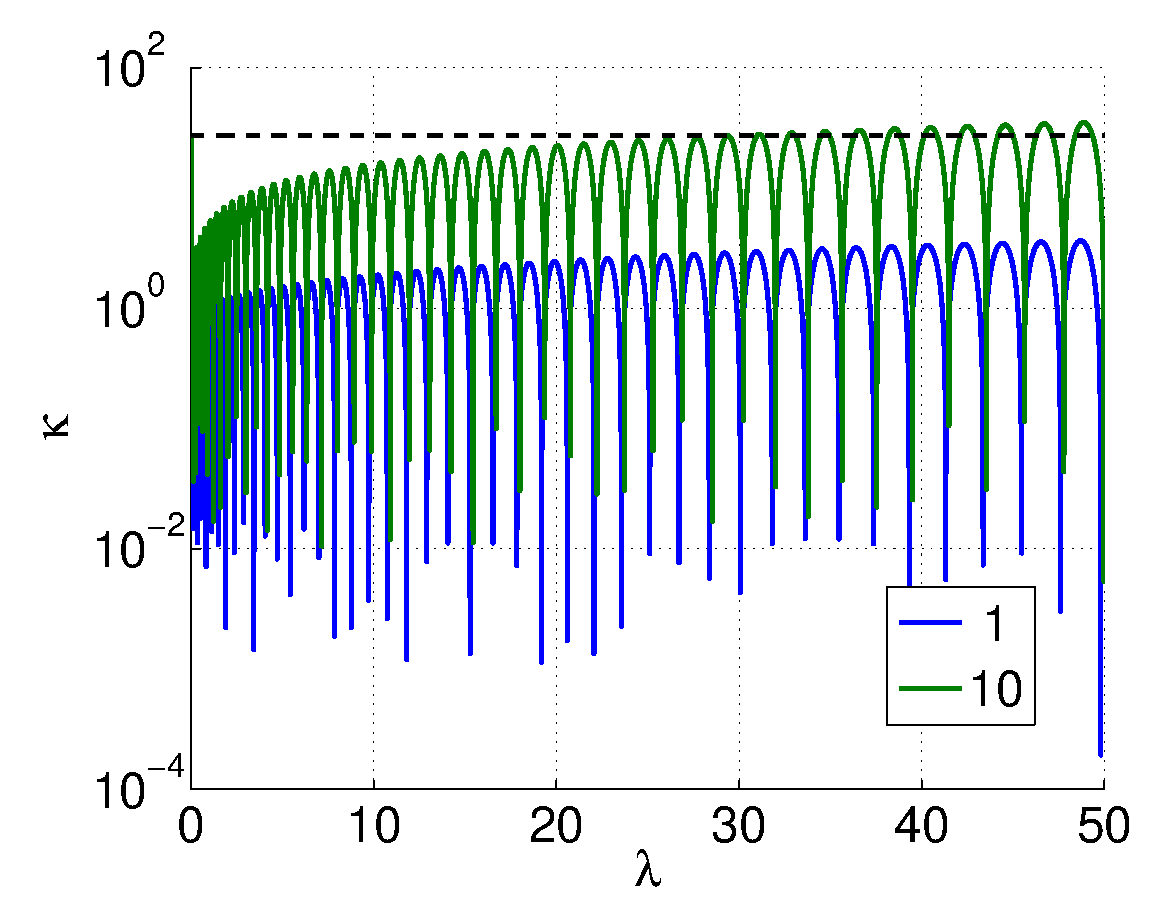
\includegraphics[height=5cm]{/Figs/kappa_nhr.eps}
%\caption{The l.h.s of \Eq{e7} for $\alpha=1$ and $\alpha=10$, $L=20, \ s=0.4$. }
%\end{figure}

%%%%%%%%%%%%%%%%%%%%%%%%%%%%%%%%%%%%%%%%%%%%%%%%%%
\clearpage

%%%%%%%%%%%%%%%%%%%%%%%%%%%%%%%%%%%%%%%%%

What is the significance of a finite gap? 
The meaning of having a "gap" is that the relaxation
is towards a localized NESS whose extension is $L$ independent.
The simplest example is $g=\infty$, for which the NESS
is concentrated in a small triangular well.
More generally if the NESS is localized we should expect a gap. 
%
In other words, if the gap vanishes then the decay times of the "non" NESS modes diverge, leading to a spatially extended NESS.


\sect{Continuous models - general}

To explain the observations we first consider three simpler continuous models of a ring of circumference $L$.
In the continuous version, the dynamics is describes by a diffusion equation with a drift term. 
%
\be{11}
\frac{\partial \psi}{\partial t} &=&\frac{\partial}{\partial x} \left[ D(x) \frac{\partial \psi}{\partial x}-v(x)\psi\right] \\
&=& \frac{\partial}{\partial x} \left[ D(x) \frac{\partial \psi}{\partial x}\right] -
 \frac{\partial}{\partial x} \left[v(x)\psi\right] 
\ee
%
Assuming that $D(x)$ and $v(x)$ are piecewise,the 
solution to the diffusion equation in each region is  simply  $\psi \sim e^{-\lambda t + ikx}$, inserting this in \Eq{e11}, we obtain the dispersion relation 
%
\beq
\lambda &=& Dk^2 + ivk \ = \ D\left(k+\frac{iv}{2D}\right)^2 + \frac{v^2}{4D} \\
k_{\pm} &=& \frac{-iv \pm \sqrt{4\lambda D -v^2}}{2D} = \frac{-is}{2} \pm \sqrt{\frac{\lambda}{D}-\frac{s^2}{4}}
\ \ \equiv \ \   \frac{-is}{2} \pm \tilde{k}
\eeq
%
So, in each region the solution to \Eq{e11} has the form 
\be{12}
\psi(x) = Ae^{ik_{+} x}+ Be^{ik_{-} x} = \eexp{\frac{v}{2D}x} \left(Ae^{i\frac{\sqrt{4\lambda D -v^2}}{2D}x}+Be^{-i\frac{\sqrt{4\lambda D -v^2}}{2D}x}\right)
\ee
%
Details regarding matching the wave functions across interfaces where there is 
a jump in the values of $v$ and $D$ are given in the appendix.
%
In the next three sections we consider several cases that are of special interest.

%There are three limiting cases which are of interest.
%In the simplest case of periodic boundary conditions and $u=0$, the eigenvalues are simply
%%
%\be{3}
%\lambda  = Dk^2 =D\frac{4\pi^2 n^2}{L^2} \ , \ n=0,1,2,...
%\ee
%%
%If there is a drift term, $u\neq 0$ (this is model I), the eigenvalues are 
%\be{4}
%\lambda &=&  D\frac{4\pi^2 n^2}{L^2}+i\frac{2\pi v}{L} n \ , \ n=0,1,2,...\\
%\lambda &=&  \frac{v^2}{4D}
%\ee
%%
%If the ring is disconnected at a point, then we have a chain and Neumann boundary conditions apply, 
%leading to the eigenvalues 
%%
%\be{5}
%\lambda &=& D\frac{\pi^2 n^2}{L^2} + \frac{v^2}{4D} \ , \ n=0,1,2,...\\ 
%\lambda &=& 0
%\ee
%%%%%%%%%%%%%%%%%%%%%%%%%%%%%%%%%%%%%%%%%%%%%%

%%%%%%%%%%%%%%%%%%%%%%%%%%%%%%%%%%%%%%%%%%%%%%
\sect{Clean ring}

The diffusion constant is constant, $D(x)=D$ and the drift velocity is $v=Ds$.
By imposing periodic boundary conditions $\psi(0)=\psi(L), \ \psi'(0) = \psi'(L)$, 
we have the secular equation 
%
\beq
\cos \left(L \sqrt{\frac{\lambda}{D} - \frac{v^2}{4D}} \right)  \ = \ \cosh  \left(\frac{v}{2D}L\right)
\eeq
%

we obtain the spectrum
%
\be{14}
\lambda &=&  D\frac{4\pi^2 n^2}{L^2}+i\frac{2\pi v}{L} n \ , \ n=0,\pm1,\pm2,...\\
\lambda &=&  \frac{v^2}{4D}
\ee
%
We see that there is a gap $\Delta = 4\pi^2/L^2$, which vanishes in the limit $L\to\infty$.
The eigenvalue $\lambda=v^2/4D$ corresponds to an evanescent mode inside the gap.
%

If the ring is disconnected at a point, then we have a chain and Neumann boundary conditions apply, 
leading to the eigenvalues 
%
\be{15}
\lambda &=& D\frac{\pi^2 n^2}{L^2} + \frac{v^2}{4D} \ , \ n=0,1,2,...\\ 
\lambda &=& 0
\ee

%%%%%%%%%%%%%%%%%%%%%%%%%%%%%%%%%%%%%%%%%%%%%%

\sect{Ring and scatterer}

\subsect{The model}

We have a ring with uniform drift velocity $u$ and a diffusive scatterer, defined as
%
\beq
D(x) = \left\{ \begin{array}{cc}
D_0, & |x|<a/2 \\
D, & |x|>a/2 
\end{array}
\right.
\eeq
%
The strength of the scatterrer can be written in dimesnionless units
%
\beq
g \ & \equiv & \ \frac{a}{L}\cdot \frac{D}{D_0} 
\eeq
%

\subsect{The secular equation}

The secular equation for the eigenvalues can be shown to be (see appendix)
%
\be{18}
\cos \left(L \sqrt{\frac{\lambda}{D}- s^2/4} \right)
%
+\frac{1}{2} \frac{aD}{D_0}\frac{\lambda}{\sqrt{\frac{\lambda}{D}-s^2/4}}\sin \left(L\sqrt{\frac{\lambda}{D}- s^2/4}\right) = \cosh\left( \frac{sL}{2}\right)
\ee
%
and in terms of dimensionless variables
%
\beq
g \ & \equiv & \ \ \frac{a}{L}\cdot \frac{D}{D_0} \\
z \ & \equiv & \ \tilde{k}L \ \ , \ \ \mathcal{S} \equiv sL \\
\lambda \ &=& \ D\left( \tilde{k}^2 + \frac{s^2}{4}\right) 
\eeq
%
the secular equation can be written as 
%
\be{19}
 \cos(z) + g \frac{z^2+(\frac{\mathcal{S}}{2})^2}{2z}\sin(z)= \cosh \left(\frac{\mathcal{S}}{2} \right)
 \ee
%


\subsect{The spectrum}

%
To characterize the spectrum vs. $s$,  it is good to keep in mind two limiting cases.
When $g=0$, we have a clean ring, and all eigenvalues are complex and they form a gapless continuum.
When $g=\infty$, we have a chain, where all the eigenvalues are real. In this case there is a gapped continuum that begins at $\Delta = s^2/4$.

For finite $g$, the spectrum is gapped, however a "bubble" of complex eigenvalues can appear in the continuum. We obtain an analytical expression for the gap
when the spectrum is real and prove that the gap is finite even when there are complex eigenvalues in the spectrum.

Let us assume that $\lambda$ is real. 
For given $\mathcal{S}$, the left hand side of the secular equation \Eq{e18} is oscilliatory, provided $\lambda > \mathcal{S}^2/4$, otherwise, the trigonometric functions become hyperbolic.
The oscillations are within an envelope function $\kappa(\lambda)$,
%
\beq
\kappa(\lambda) = \sqrt{1+ \frac{g^2\lambda^2 }{4\lambda-\mathcal{S}^2}}
\eeq
%
There are real solutlons to the secular equation as long as the envelope function satisfies
\beq
\kappa(\lambda) > \cosh\left( \frac{\mathcal S}{2}\right)
\eeq
%
which leads to the expression for the gap, provided that the spectrum is entirely real (\Fig{lambda_star}),
%
\be{17}
\text{Re}[\lambda] \geq \frac{2 \sinh^2(\mathcal{S}/2)}{g} \left[ 1 + \sqrt{1- \frac{g^2 \mathcal{S}^2}{4\sinh^2(\mathcal{S}/2)}}\right] \ \ =  \ \ \Delta(s)
\ee
%

\begin{figure}[h]
\includegraphics[height=7cm]{real_lambda_contour.eps}
\caption{The real part of the eigenvalues for an $L=100, \ D=1$ ring with a single diffusion barrier with 
$g=10^3$ plotted vs. the affinity $s$.
The dashed black line is  \Eq{e17}, which is the value of the gap and also indicates where the eigenvalues become complex.
Notice that at the bottom of the band there is an eigenvalue that is always real.
This plot was generated by producing a contour plot of \Eq{e18} for real $\lambda$'s, it shows only real eigenvalues.
}
\label{lambda_star}
\end{figure}

When $\mathcal{S}$ increases such that  $\cosh(\mathcal{S}/2)>\kappa(\lambda)$, a complex "bubble" of eigenvalues appears.
The bubble structure is due to the fact that the envelope function $\kappa(\lambda)$ has a global minimum at 
$\lambda_{\min}=\mathcal{S}^2/2$, so for  $\lambda > \lambda_{\min}$ the envelope function grows monotonically and will eventually intersect with $\cosh(\mathcal{S}/2)$.
This scenario is illustrated in \Fig{fig_f}.
%
The minimum value of the envelope function is
%
\beq
  \kappa_{\text{min}} =\sqrt{ 1+\left(\frac{g\mathcal{S}}{2}\right)^2}
\eeq
%
The critical value $\mathcal{S}_g$ such that for $\mathcal{S}>\mathcal{S}_g$ there are complex
eigenvalues in the spectrum is determined by the transcendental equation 
%
\beq
 1+\left(\frac{g\mathcal{S}}{2}\right)^2 \ =  \ \cosh^2\left( \frac{\mathcal{S}}{2} \right)
\eeq
%
%
%
\begin{figure}[h]
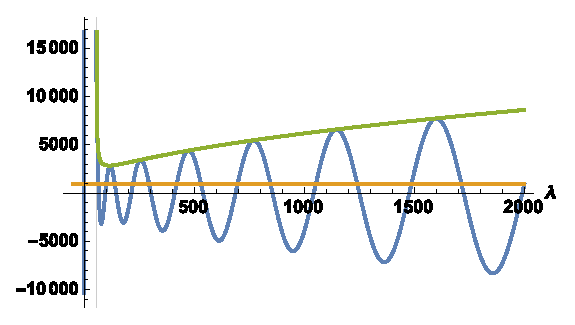
\includegraphics[width=7cm]{gRing3.eps}
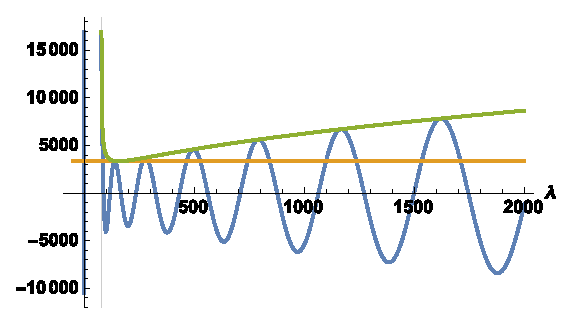
\includegraphics[width=7cm]{gRing2.eps}

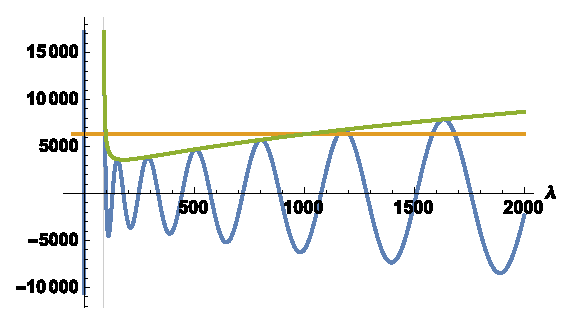
\includegraphics[width=7cm]{gRing1.eps} 

\ \ \ \  \ \ \includegraphics[width=6cm]{gRing1Diagram}
%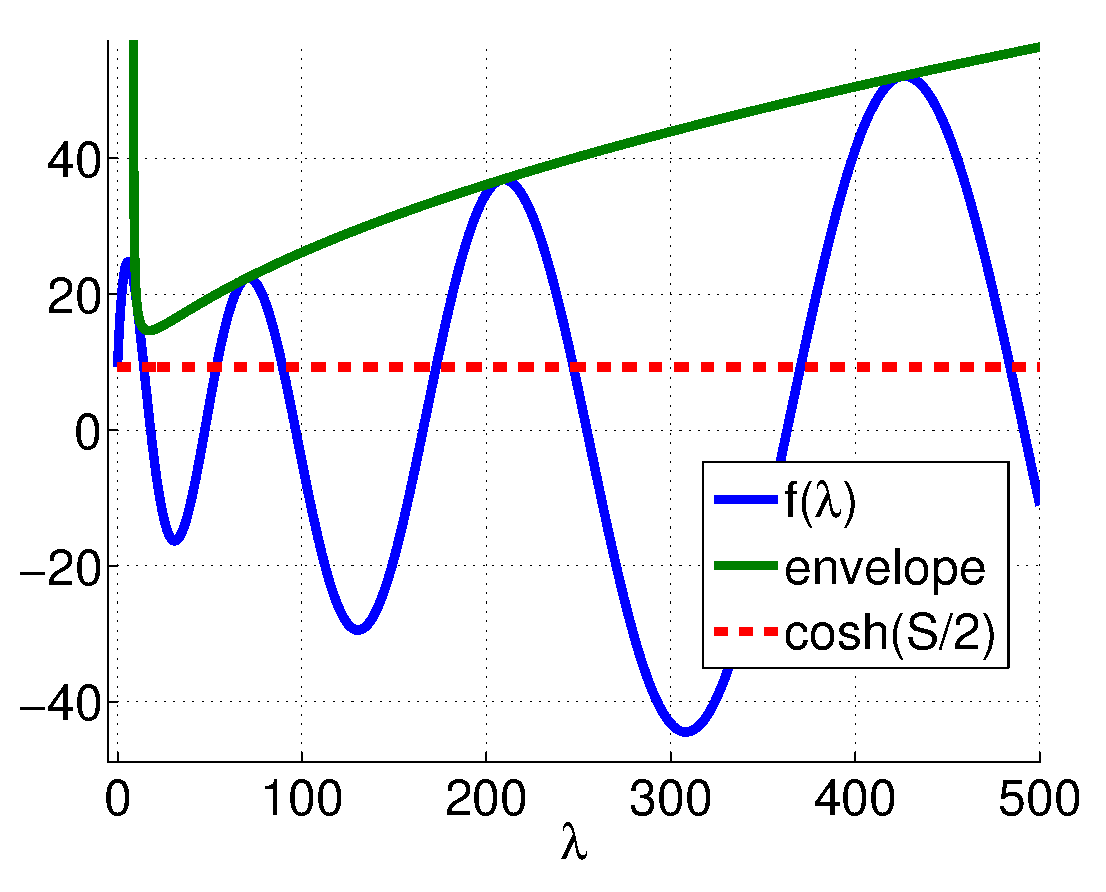
\includegraphics[height=4cm]{f_sg_m.eps}
%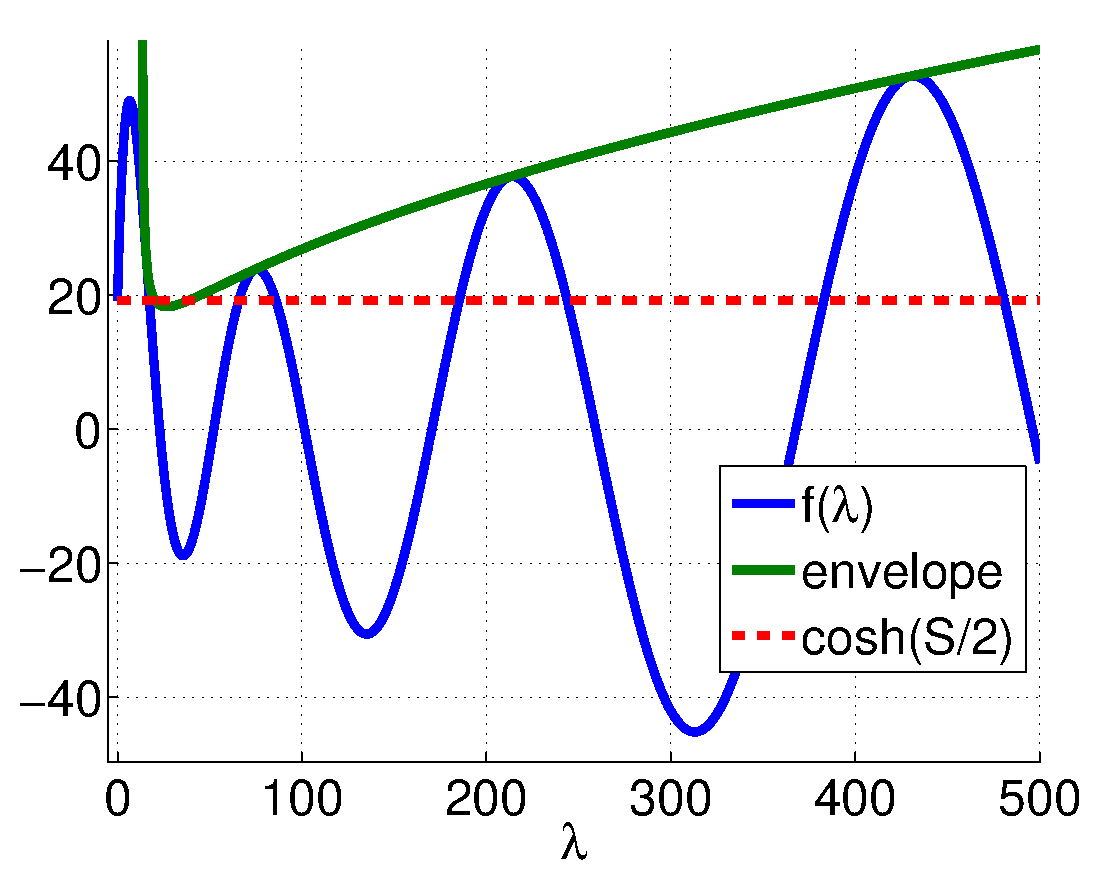
\includegraphics[height=4cm]{f_sg.eps}
%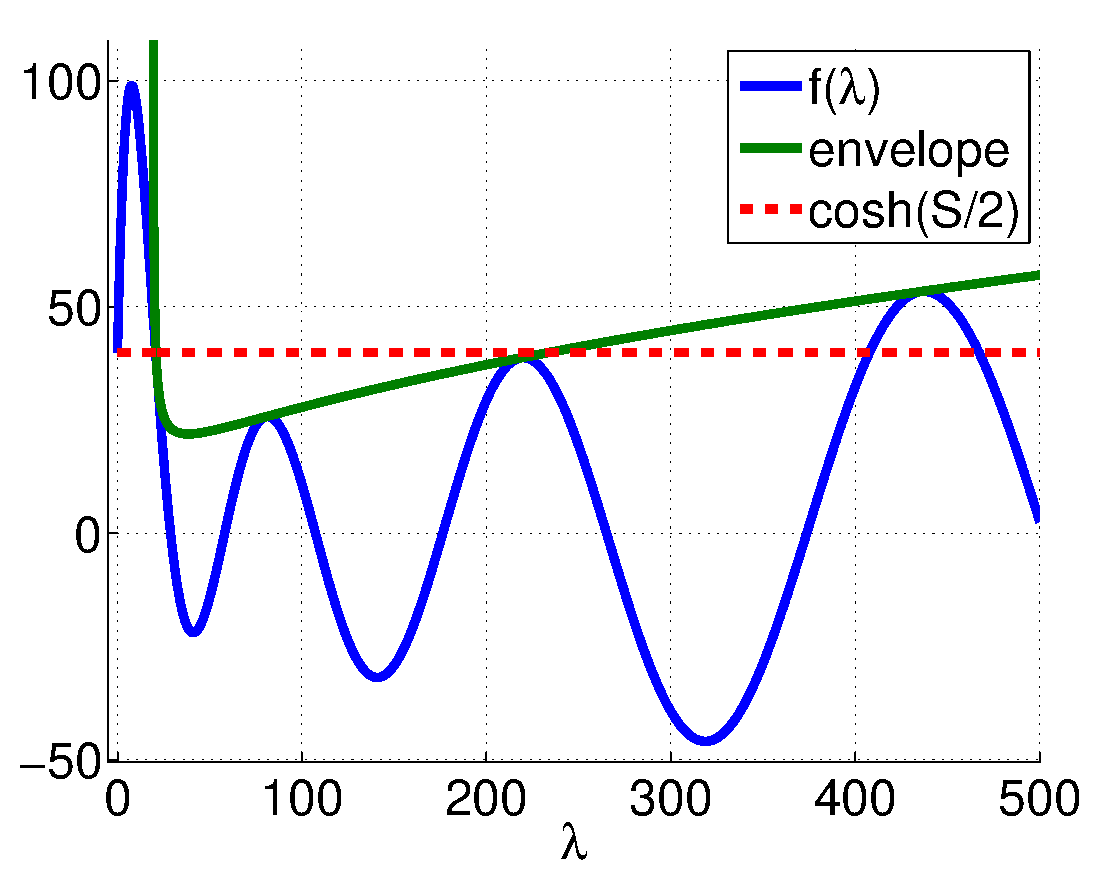
\includegraphics[height=4cm]{f_sg_p.eps}
\caption{
The secular equation $f(\lambda)=\cosh(\mathcal{S}/2)$ for $g=380$, so $\mathcal{S}_g=17.6$.
Top row:  (left)  $\mathcal{S} =15$ , all eigenvalues are real. 
(right) $\mathcal{S} = \mathcal{S}_g$, marginal case.
Middle row:l $\mathcal{S} = 19$, the fully developed scenario, where the spectrum is initially real, then there is a "bubble" of complex eigenvalues and then the spectrum becomes real again. The high eigenvalues correspond to modes that decay very fast. Intuitively, since the high eigenvalues decay quickly, they cannot complete a trip around the ring before they decay, so they must be real. 
The blue line is the oscillating part of the secular equation. The green line is the envelop function and 
the horizontal orange line is $\cosh(\mathcal{S}/2)$.
In the bottom row we draw a schematic diagram of the spectrum in the complex plane of $\lambda$,
corresponding to the fully developed scenario.}
\label{fig_f}
\end{figure}

%%%%%%%%%%%%%%%%%%%
\subsect{Proof the gap is finite}

To show that the gap remains finite even when there are complex eigenvalues, it is more convenient 
to use the second form of the secular equation 
where the wave vector is  $z=x+iy$.
 The eigenvalues can be expressed in the following form 
 %
 \beq
\lambda = (x+iy)^2+\left(\frac{\mathcal{S}}{2}\right)^2 = x^2-y^2 + \left(\frac{\mathcal{S}}{2}\right)^2 +2ixy
\eeq
%
There is a trivial eigenvalue at $x=0, \ y=\mathcal{S}/2$. 
To show that the gap is finite, 
it is sufficient to show that for $x\neq 0$,  $y<{\mathcal{S}}/{2}$.
Inserting $z=x+iy$, the secular equation splits in to two equations (for real and imaginary parts).
%
The real part of equation \Eq{e19} is 
%
\be{20}
\cos (x) \left[ \cosh (y) - gy \sinh (y) \frac{x^2+y^2 - \mathcal{S}^2/4}{2(x^2+y^2)} \right]
+\sin(x) \left[ gx \cosh(y)\frac{x^2+y^2 + \mathcal{S}^2/4}{2(x^2+y^2)}   \right]
= \cosh\left(\frac{\mathcal{S}}{2}\right)
\ee
%
This equation has the form $A(x,y) \sin(x) + B(x,y) \cos(x) = \cosh(\mathcal{S}/2)$.
For finite $x=x_1$, $y_1$ is determined by the 
condition that the envelope of the function intersects with $\cosh(\mathcal{S}/2)$
%
\beq
\sqrt{A^2+B^2} = \cosh(\mathcal{S}/2)
\eeq
%
To prove that $y_1 < \mathcal{S}/2$ it is enough to show that for $y=\mathcal{S}/2$ the envelope satisfies
$\sqrt{A^2+B^2} > \cosh(\mathcal{S}/2)$.
Assume that $g\gg 1$ and $\mathcal{S} \gg \mathcal{S}_g$, in this case there is a large bubble of complex eigenvalues so the gap is complex. Also, we can approximate 
$\cosh y \approx \sinh y \approx e^y$ 
and 
$\cosh(\mathcal{S}/2)\approx e^{\mathcal{S}/2}$.
%
In this limit the envelope is 
%
\beq
\left. \frac{g}{2} e^y \sqrt{x^2+y^2} \sqrt{1+ \frac{\mathcal{S}^2(x^2-y^2+\mathcal{S}^2)}{2(x^2+y^2)}} \right|_{y=\mathcal{S}/2} = \ \
\frac{ge^{\mathcal{S}/2}}{2}
\sqrt{x^2+(\mathcal{S}/2)^2}
\sqrt{1+\frac{\mathcal{S}^2(x^2+3(\mathcal{S}/2)^2)}{2(x^2+(\mathcal{S}/2)^2)}} \ \ > \ \ e^{\mathcal{S}/2}
\eeq
%
so the solution must be $y<\mathcal{S}/2$.
%

%%%%%%%%%%%%%%%%%%%%%%%%%%%%%%%%%%%%%%%%%%%%%%
\sect{Ring and $\sigma$}

\subsect{The model}

The ring is divided in to two segments with drift velocities defined
%
\beq
v(x) = \left\{ \begin{array}{cc}
v_1 \ =\  D(s+\sigma), & 0< x<L/2 \\
v_2 \ = \ D(s-\sigma)\ , & L/2<x<L
\end{array}
\right.
\eeq

\subsect{The secular equation}

The secular equation for the eigenvalues can be shown to be (see appendix)
%
\be{20}
\cosh\left(\frac{\mathcal{S}}{2}\right) &=&
\cos \left(\frac{L}{4} \sqrt{4 \lambda -(s-\sigma )^2}\right) 
\cos \left(\frac{L}{4} \sqrt{4 \lambda -(s+\sigma )^2}\right)-\\
&-&\frac{\left(4 \lambda -s^2+\sigma ^2\right)}{\sqrt{4 \lambda -(s-\sigma )^2} \sqrt{4 \lambda -(s+\sigma )^2}}
 \sin \left(\frac{L}{4} \sqrt{4 \lambda -(s-\sigma )^2}\right) 
 \sin \left(\frac{L}{4} \sqrt{4 \lambda -(s+\sigma )^2}\right)
\ee
%
or, in terms of dimensionless variables,
$\mathcal{S}=sL, \ \ \sigma := \sigma L$
%
\be{21}
\cosh\left(\frac{\mathcal{S}}{2}\right) &=&
%\cos\left[\frac{1}{2}\sqrt{z^2-\left(\frac{\sigma}{2}\right)^2 - \frac{\sigma s}{2}}\right]
%\cos\left[\frac{1}{2}\sqrt{z^2-\left(\frac{\sigma}{2}\right)^2 + \frac{\sigma s}{2}}\right]\\
%&-&\frac{z^2+\left(\frac{\sigma}{2}\right)^2}{\sqrt{\left(z^2-\left(\frac{\sigma}{2}\right)^2\right)^2-\left(\frac{\sigma s}{2}\right)^2}}
%\sin\left[\frac{1}{2}\sqrt{z^2-\left(\frac{\sigma}{2}\right)^2 - \frac{\sigma s}{2}}\right]
%\sin\left[\frac{1}{2}\sqrt{z^2-\left(\frac{\sigma}{2}\right)^2 + \frac{\sigma s}{2}}\right] = \\
%&=&
\cos\left[\frac{1}{2}\sqrt{z^2-\left(\frac{\sigma}{2}\right)^2 - \frac{\sigma \mathcal{S}}{2}}\right]
\cos\left[\frac{1}{2}\sqrt{z^2-\left(\frac{\sigma}{2}\right)^2 + \frac{\sigma \mathcal{S}}{2}}\right]-\\
&-&\left(z^2+\left(\frac{\sigma}{2}\right)^2\right)
\frac{\sin\left[\frac{1}{2}\sqrt{z^2-\left(\frac{\sigma}{2}\right)^2 - \frac{\sigma \mathcal{S}}{2}}\right]}{\sqrt{z^2-\left(\frac{\sigma}{2}\right)^2 - \frac{\sigma \mathcal{S}}{2}}}\
\frac{\sin\left[\frac{1}{2}\sqrt{z^2-\left(\frac{\sigma}{2}\right)^2 +\frac{\sigma \mathcal{S}}{2}}\right]}{\sqrt{z^2-\left(\frac{\sigma}{2}\right)^2 + \frac{\sigma \mathcal{S}}{2}}}  \nonumber
\ee
%


\subsect{The spectrum}

We first consider two limiting cases, $\mathcal{S} = 0$ and $\mathcal{S}\gg \sigma$ and then the general case.
For $\mathcal{S}=0$, the secular equation can be written as 
%
\be{22}
\tan^2 \left(\frac{1}{4}\sqrt{4\lambda - \sigma^2}\right) \ = \ \frac{4\lambda - \sigma^2}{4\lambda + \sigma^2}
\ee
%
There is the trivial solution at $\lambda=0$, the next solution is at $\lambda = \sigma^2/4$ so there is a finite gap independent of $L$, followed by a "continuum", see \Fig{sigmaRing_s_0}.

For $\mathcal{S}\gg \sigma$, we neglect $\sigma$ in the secular equation and obtain the 
secular equation for a clean ring, 
%
\beq
 \cos \left ( \frac{1}{2} \sqrt{4\lambda - \mathcal{S}^2} \right) = \cosh\left(\frac{\mathcal{S}}{2}\right) 
\eeq
%
That is, the spectrum is gapless ($\Delta \sim 1/L^2$) and complex.

%
For intermediate values of $\mathcal{S}$, the spectrum can be divided in to three regions.
For ${\lambda > (\mathcal{S}+\sigma)^2/4}$, all the trigonometric functions are oscillatory, resulting in a continuum. Since the envelope function is bounded in this region, the eigenvalues are complex.
%

For ${(\mathcal{S}-\sigma)^2/4 \ < \  \lambda \ < \ (\mathcal{S}+\sigma)^2/4}$ the trigonometric 
functions whose argument is ${\sqrt{\lambda - (\mathcal{S}+\sigma)^2/4}}$ become hyperbolic.
The oscillations ensure that the eigenvalues for a continuum, and the hyperbolic functions 
form an envelope that is unbounded, so the eigenvalues may be real, depending on $\mathcal{S}$.
In order for there to be real eigenvalues, there must be oscillations, this happens only if $\sigma>4\pi$.
The envelope function is 
%
\beq
\kappa(\lambda)=\left(
\left[
\cosh \left(\frac{1}{4} \sqrt{|4\lambda - (s+\sigma)^2|}\right) 
\right]^2+ 
\left[
\sinh \left(\frac{1}{4} \sqrt{|4\lambda - (s+\sigma)^2|}\right)
\frac{\left(4 \lambda -s^2+\sigma ^2\right)}{\sqrt{4 \lambda -(s-\sigma )^2} \sqrt{|4 \lambda -(s+\sigma )^2|}}
\right]^2
\right)^{1/2}
\eeq
%
%In this region the secular equation is of the form $A\cos(x) +B\sin(x)=\cosh(\mathcal{S}/2)$, so an envelope function can be written.
%

For ${\lambda \ < \   (\mathcal{S}-\sigma)^2/4}$ all the terms are hyperbolic, so there is at most one solution in this region.
%

The gap decreases from $\sigma^2/4$ to $(\mathcal{S}-\sigma)^2/4$ until some point $\mathcal{S} = \sigma - \epsilon$, 
then the gap becomes complex and increases until $\mathcal{S}=\sigma$ from which point the gap closes. I don't know how to determine $\epsilon$, however it arises because at $\mathcal{S}=\sigma$, the envelope is equal to $\cosh(\mathcal{S}/2)$ at $\lambda = 0$ and is a monotonically decreasing function of $\lambda$. Thus the first non trivial solution is for $\mathcal{S}<\sigma$. In any case, this solution is part of the continuum so we can deduce that $\epsilon \sim 1/L^2$. 

%
\begin{figure}[h]
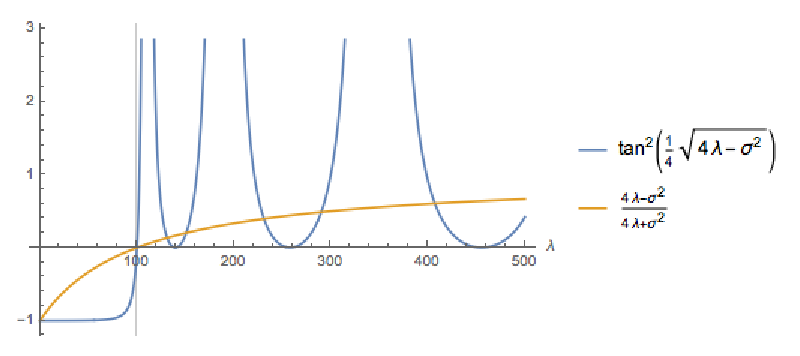
\includegraphics[height=4cm]{sigmaRing_s_0}
\caption{Graphical solution of the secular equation \Eq{e22} for $\mathcal{S}=0$ and $\sigma=20$, depicting the finite gap at $\lambda = 100$}
\label{sigmaRing_s_0}
\end{figure}
%
\begin{figure}[h]
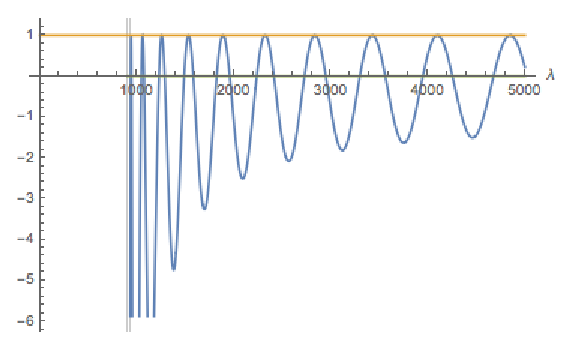
\includegraphics[width=5cm]{sigmaRing_gap_real_continuum}
%
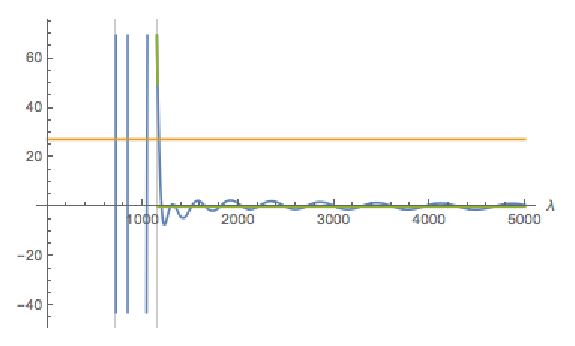
\includegraphics[width=5cm]{sigmaRing_gap_real_complex}
%
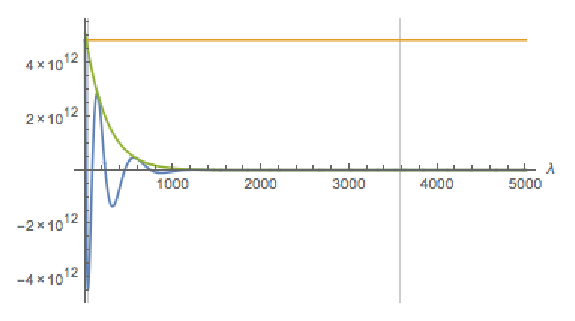
\includegraphics[width=5cm]{sigmaRing_complex}
\caption{
Graphical representation of the secular equation. The horizontal orange line is $\cosh(\mathcal{S}/2)$.
Top: $\mathcal{S}=0$ (corresponds to \Fig{sigmaRing_s_0}), there is a gap $\Delta=\sigma^2/4$ between $\lambda=0$ and a real continuum,
Middle: $\mathcal{S}<\sigma$, there is a gap, followed by a real continuum, followed by a complex continuum.
Bottom: $\mathcal{S}=\sigma$ the gap vanishes, followed by a complex continuum.
}
\end{figure}
%
\begin{figure}[h]
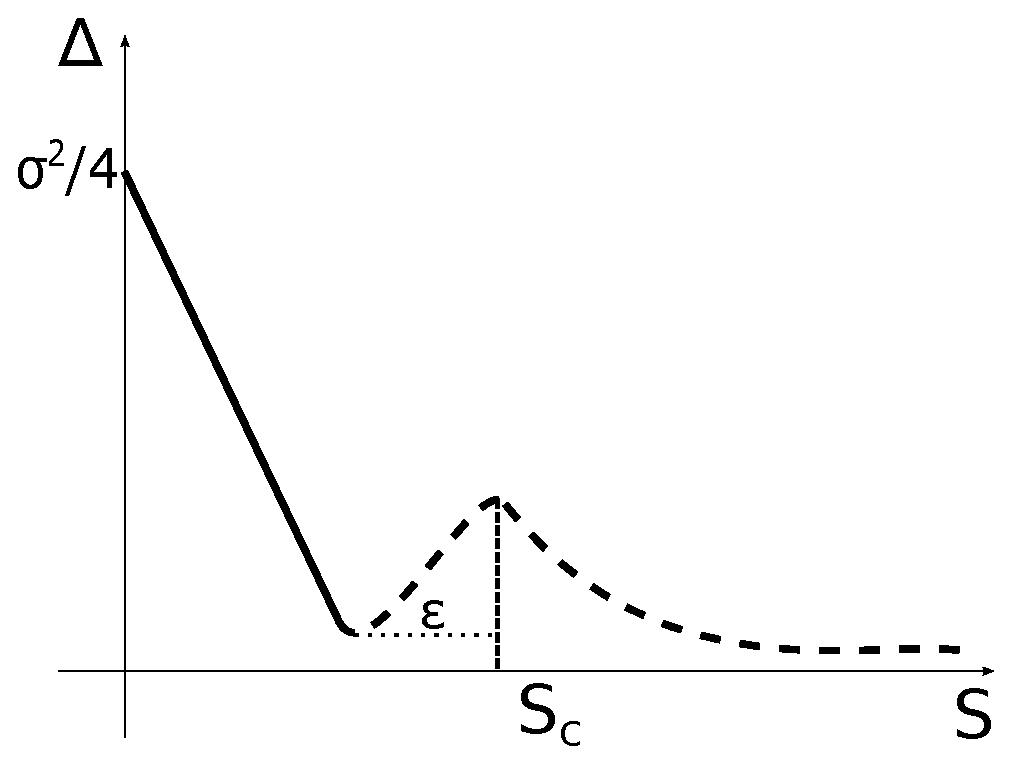
\includegraphics[height=5cm]{gap_drawing.eps}
\caption{Schematic drawing of the gap $\Delta$ vs. $\mathcal{S}$. Solid line indicates a real gap, dashed line indicates a complex gap.}
\end{figure}


%%%%%%%%%%%%%%%%%%%%%%%%%%%%%%%%%%%
\clearpage
\sect{Tight binding models}

In this section we present the results for the corresponding tightbinding models.

\subsect{Tight binding clean ring}

Consider a discrete lattice of length $L$ with lattice constant $a$, such that $L=Na$. Periodic boundary conditions are imposed.
The rate equation is diagonal in the momentum basis, thus the dispersion relation for a clean ring is given by
%
\beq
\lambda(k) \  = \ 2\cos\left( ika + \frac{sa}{2}\right) - 2\cosh\left(\frac{sa}{2}\right)
\eeq
%
The dispersion relation can be inverted to obtain $k_{\pm}$ (we take the first branch)
%
\beq
k_{\pm} \ = \ \frac{is}{2} \pm \frac{1}{a} \arccos \left[ \frac{\lambda}{2} + \cosh\left(\frac{sa}{2}\right) \right]
\eeq
%
The secular equation for periodic boundary conditions is just as in the continuous model, 
%
\beq
\left( k_{-}-k_{+}\right) \left(1- e^{ik_-L} - e^{ik_+L}  + e^{i(k_- + k_+) L}\right) =0
\eeq
%
Which yields the equation,
%
\beq
\cos \left[ \frac{L}{a} \arccos \left(\frac{\lambda}{2} + \cosh\frac{sa}{2} \right) \right] \  &=& \ \cosh\left(\frac{sL}{2}\right)
\eeq
%
The solutions are
%
\be{23}
\lambda_n  \ &=& \ 2\cosh\left(\frac{\mathcal{S}}{2N}\right) \left[ \cos \left(\frac{2\pi n}{N}\right) - 1\right] 
+ 2i \sinh\left(\frac{\mathcal{S}}{2N}\right)  \sin \left(\frac{2\pi n}{N}\right) 
\ee
%
where $s = \mathcal{S}/Na$.
The gap is give by the first non zero eigenvalue
%
\be{24}	
\Delta = \lambda_1 & \approx & \frac{4\pi^2}{N^2}\cosh \left(\frac{as}{2}\right) + i \frac{4\pi}{N}\sinh \left(\frac{as}{2}\right) 
\ee
%
%%%%%%%%%%%%%%%%%%%%
%\rmrk{
%Note that there is an additional equation
%%
%\beq
%\arccos\left[ \frac{\lambda}{2} + \cosh\left(\frac{sa}{2}\right) \right] \ &=& \ 0
%\eeq
%%
%which has solutions
%%
%\beq
%\lambda_n = -2\cosh\left(\frac{\mathcal{S}}{2N}\right) +(2n+1)\pi
%\eeq
%%
%however, this solution does not appear in the numerical diagonalization. 
%}
%%%%%%%%%%%%%%%%%%%%

\clearpage

\subsect{Tight binding ring+$g$}

\begin{figure}[h]
\includegraphics[height=5cm]{ReLambda_s_1.eps}
\includegraphics[height=5cm]{ImLambda_s_1.eps}
\caption{The eigenvalues for an $N=25$ ring with a single diffusion barrier with $g=\exp(-7.5)$ plotted vs. the affinity $s$.}
\label{discrete}
\end{figure}


\subsect{Tight binding ring + $\sigma$}

\begin{figure}[h]
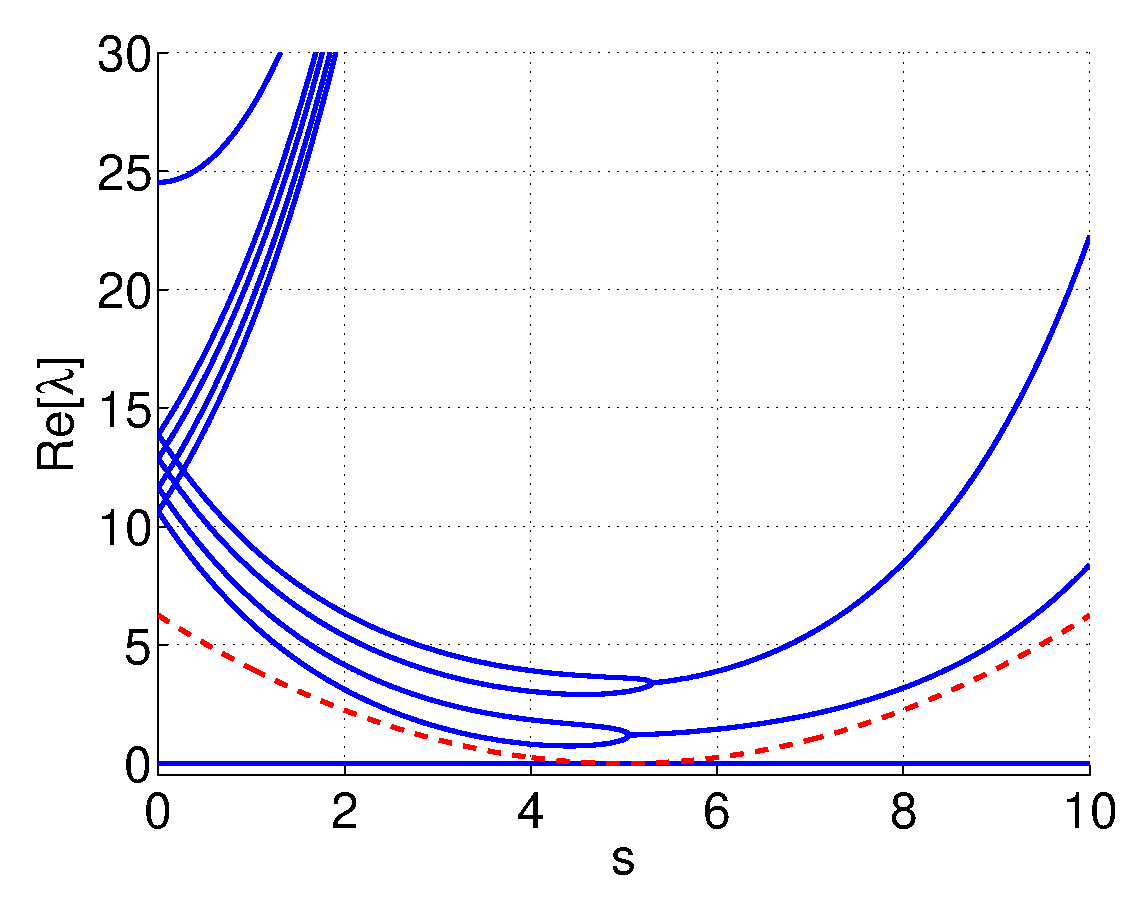
\includegraphics[height=5cm]{realLambda_sigma_5}
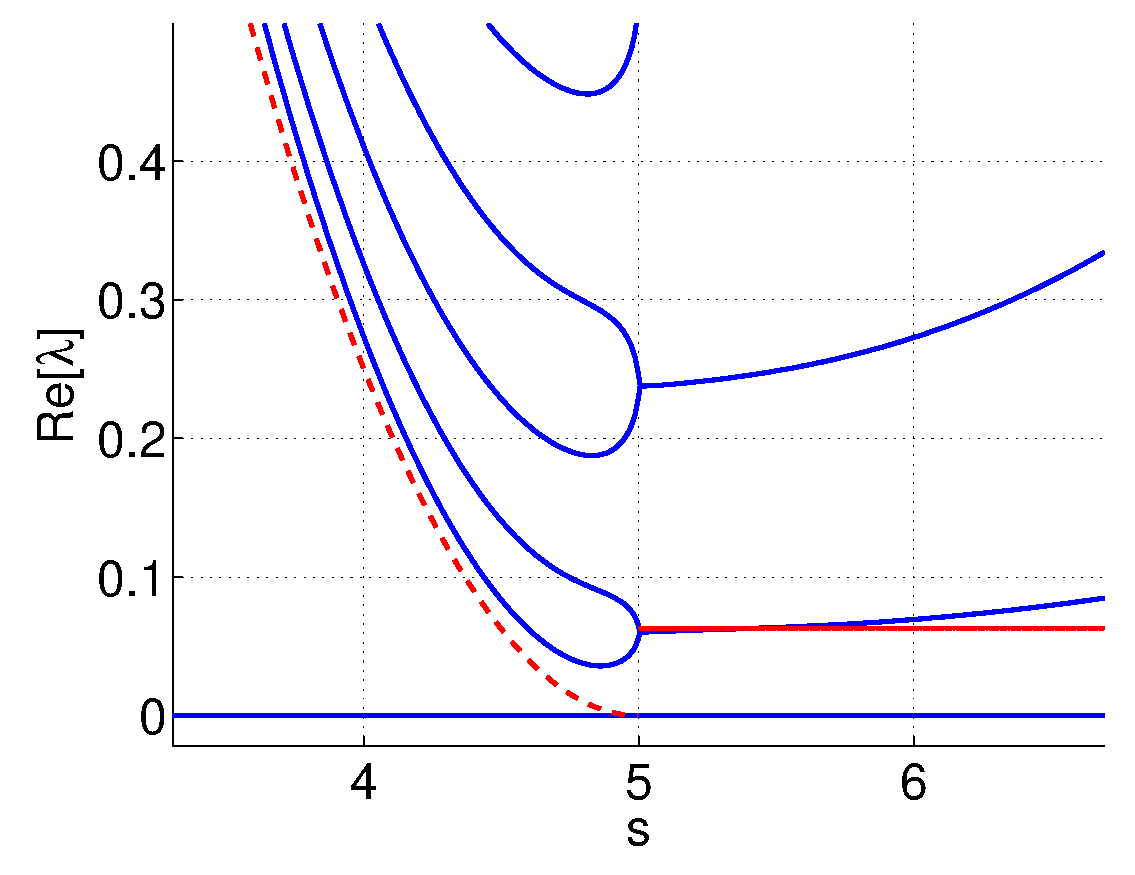
\includegraphics[height=5cm]{realLambda_sigma_5_N_50}
\caption{Left panel: The eigenvalues for an $N=10$ ring with two drift regions $\sigma=5$ plotted vs. the affinity $s$. Right panel: The same, but for $N=100$, focusing on the lower bands.
%The dashed red line corresponds to the solution $z_1$ of \Eq{e15}, the deviation is because of the tight binding approximation (finite size effect). 
The horizontal red line is $\text{Re}[\lambda] = 16\pi^2D/N^2$.}
\label{realSpectrum}
\end{figure}


%%%%%%%%%%%%%%%%%%%%%%%%%%%%
\subsect{Tight binding ring +  well}

We consider a ring that has a triangular well with slope $\sigma$.


\begin{figure}[h]
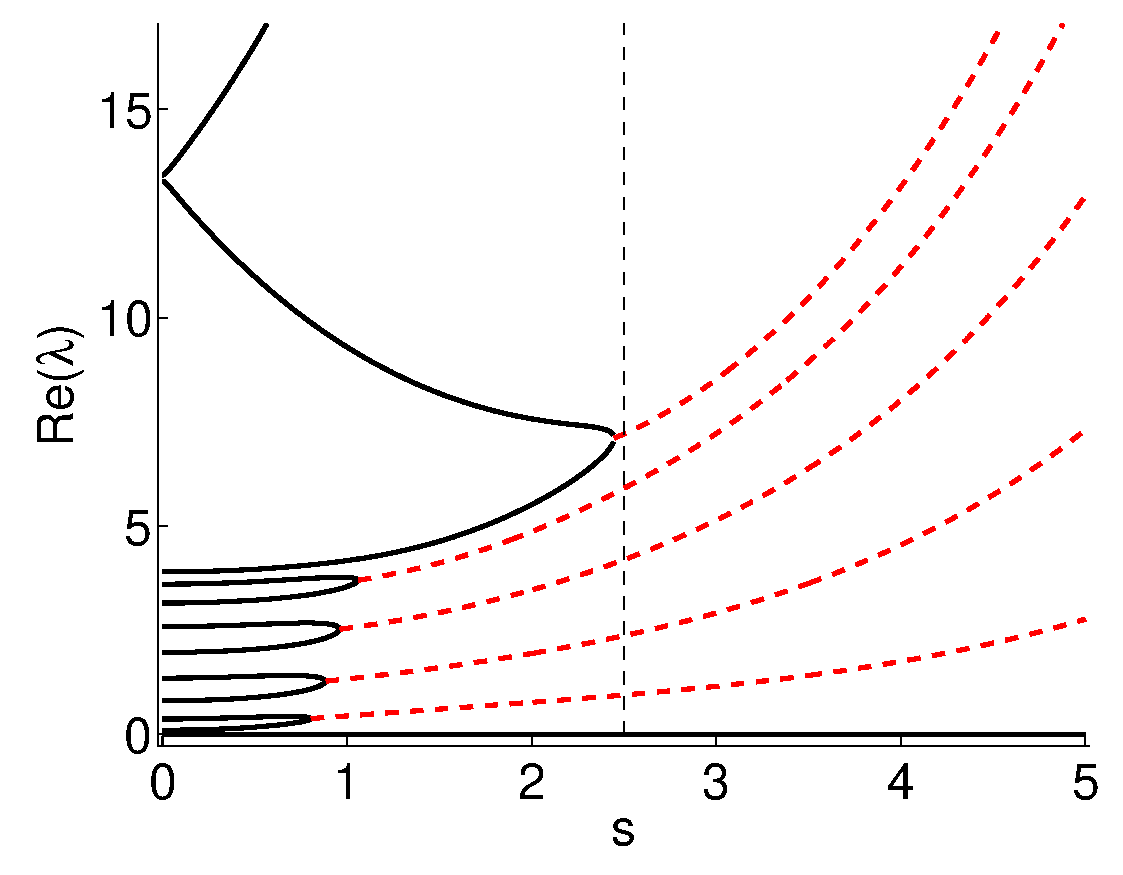
\includegraphics[height=5cm]{tbWell_real}
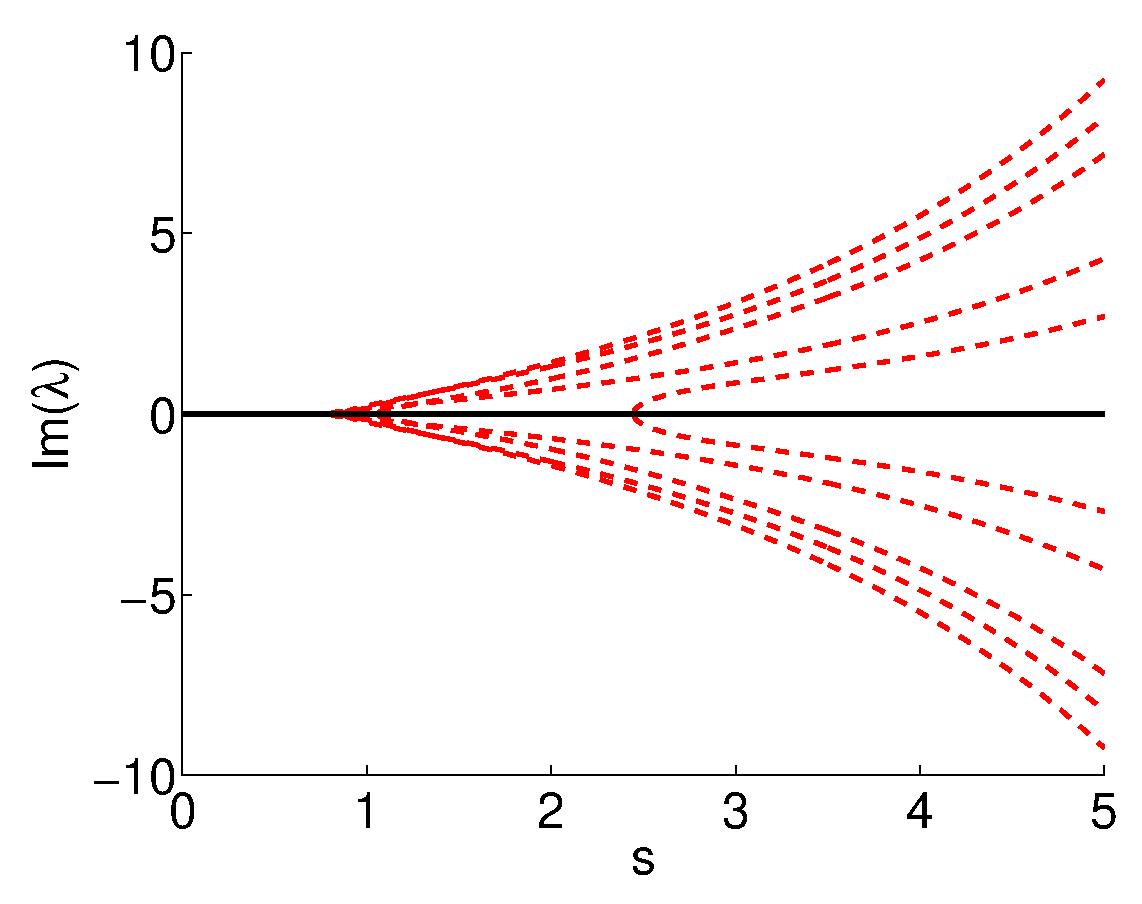
\includegraphics[height=5cm]{tbWell_imag}
\caption{Left panel: The eigenvalues for an $N=12$ ring with a well with slope $\sigma=5$ plotted vs. the affinity $s$. Solid black lines indicate the eigenvalues are real. Dashed red indicate they are complex.}
\label{realSpectrum}
\end{figure}

%
%%%%%%%%%%%
%\begin{figure}[h]
%%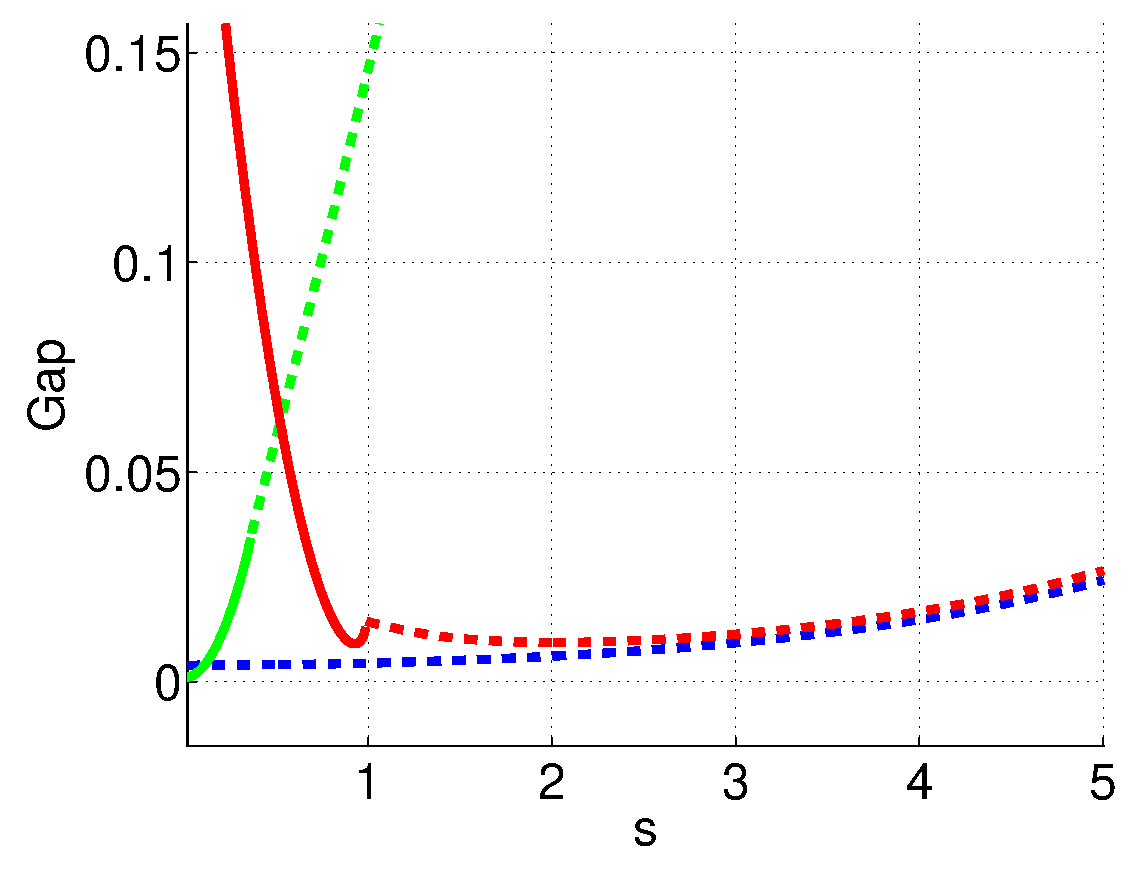
\includegraphics[height=5cm]{/Figs/gap_s_I_II_III_N_100_2.eps}
%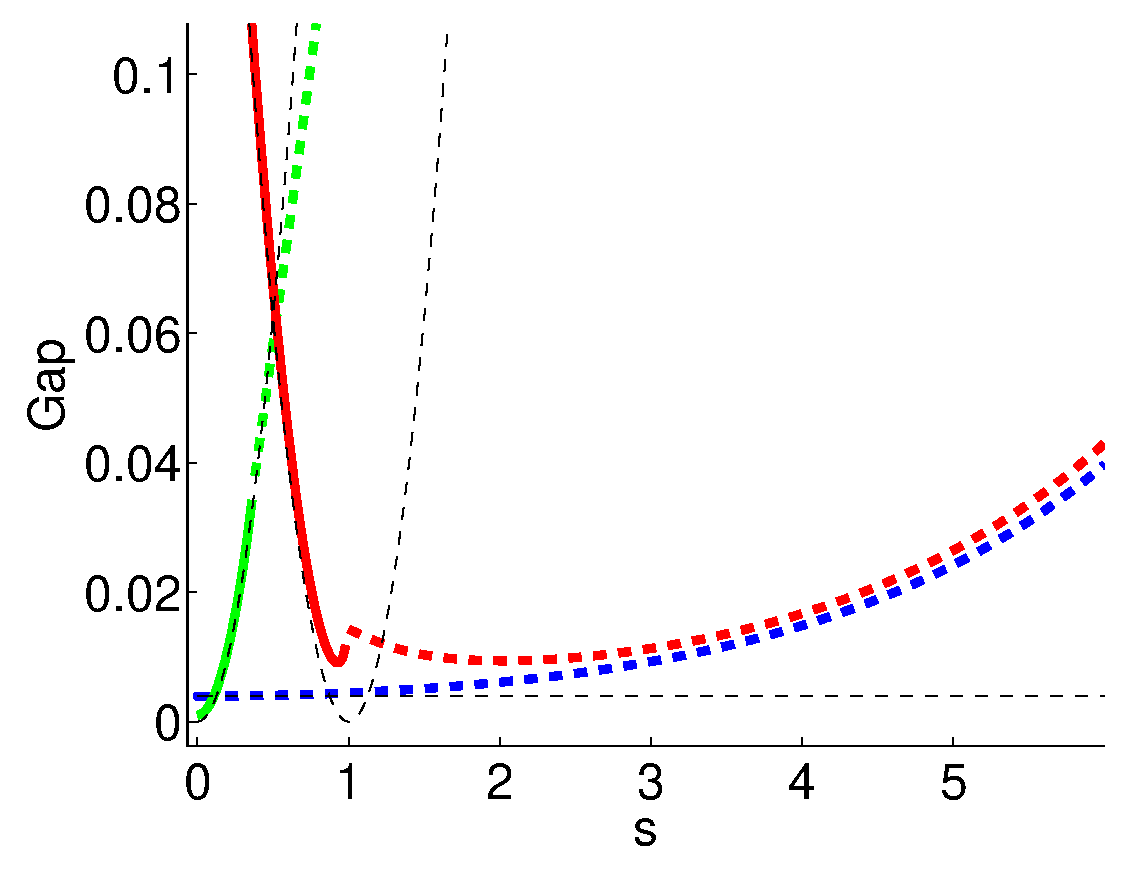
\includegraphics[height=5cm]{/Figs/gap_s_I_II_III_N_100_4.eps}
%\caption{The gap in the spectrum vs. the affinity $s$ for models I (blue) ,II (green) and III (red) as described in the text. 
%Here $N=100$. Solid lines indicate that the gap is real, dotted lines indicate the gap is complex. 
%For model I (blue) we have $\sigma=0$ and $g=1$. For model II (green) we have $\sigma =0$ and $g=10^{-8}$. For model III (red) we have $\sigma = 1$ and $g=1$.
%The horizontal black line is $\lambda=4\pi^2/N^2$, the black dotted parabolas  $s^2/4$ and $(s-\sigma)^2/4$.
%\rmrk{I do not understand why $v^2/4D$ doesn't show up in the tight binding model...}
%}
%\label{fig12}
%\end{figure}
%

\clearpage
%%%%%%%%%%%%%%%%%%%%%%%%%%%%%%%%%%%%%%%%
\sect{Tight binding with disorder}

%%%%%%%%%%%%%%%%%%%%%%%%%%%%%%%%%%%%%%%%
\subsect{The model}


Below we consider a 1D model were we have an interplay of resistor-network physics 
(due to random couplings) and Sinai physics (due to random stochastic field).       
Specifically we consider an $N$ site ring with near-neighbor transitions.
Each bond is characterized by two numbers:
%
\be{1}
\mathcal{B}_n \ \ &=& \ \ \text{barriers} \ \ = \ \ \text{random} \in [-\Delta,\Delta] \\
\mathcal{E}_n \ \ &=& \ \ \text{stochastic field} \ \ = \ \ \text{random} \in [s-\sigma,s+\sigma] 
\ee
%
Accordingly the transition rates across the $n^{th}$ bond are 
%
\be{1}
\ora{w}_{n} &=&  w_{n+1,n} \ = \ g_n \eexp{ \mathcal{E}_n/2} \ = \ \eexp{-\mathcal{B}_n + \mathcal{E}_n/2} \\
\ola{w}_{n} &=&  w_{n,n+1} \ = \ g_n \eexp{-\mathcal{E}_n/2} \ = \ \eexp{-\mathcal{B}_n - \mathcal{E}_n/2}
\ee
%
The average stochastic field~$s$ is called in the literature ``affinity". 
It can be written as $s=\text{Force}/T$, where the force 
is defined as the slope of the potential, and $T$ is the temperature.
The term ``slope" is appropriate if we view our model as describing 
a periodic lattice with $N$-site unit cell. But we prefer to have in 
mind a ring geometry so the more appropriate notion is ``stochastic motive force":
%
\beq
\mathcal{S} \ \ = \ \ \sum_{n\in\text{ring}}^N \mathcal{E}_{n} \ \ = \ \ Ns
\eeq  
%

%%%%%%%%%%%%%%%%%%%%%%%%%%%%%%%%%%%%%%%%
\subsect{Main observations}

It is known from the work of Derrida \cite{odh1} that there are "phase transitions" when
%
\be{2}
\left\langle \left( \frac{\ora{w}}{\ola{w}}\right)^{\mu} \right\rangle =1
\ee
%
For our log-box model of disorder this equation becomes (see \Fig{s_mu}).
%
\be{3}
s_{\mu} = \frac{1}{\mu}\ln\left(\frac{\sinh(\mu\sigma)}{\mu\sigma}\right)
\ee
%
For example, for $\mu=1/2$ the diffusion coefficient goes from sub ohmic to super ohmic, for $\mu=1$ there is a transition from $v=0$ to finite $v$ and 
For $\mu=2$ there is a transition from $D=\infty$ to finite $D$.
These are properties of the steady state, yet remarkabely they
have fingerprints on the relaxation process as well.
For example, if we count the number of complex eigenvalues vs. $s$ we see that
not all of the eigenvalues become complex. 
The spectrum begins to show complexity at $s_{1/2}=$ and the number of complex eigenvalues 
saturates at $s_{1}$. 
We call this "complexity saturation".
%%%%%%%%%%%%%%%%%%%%%%%%%
\begin{figure}[h]
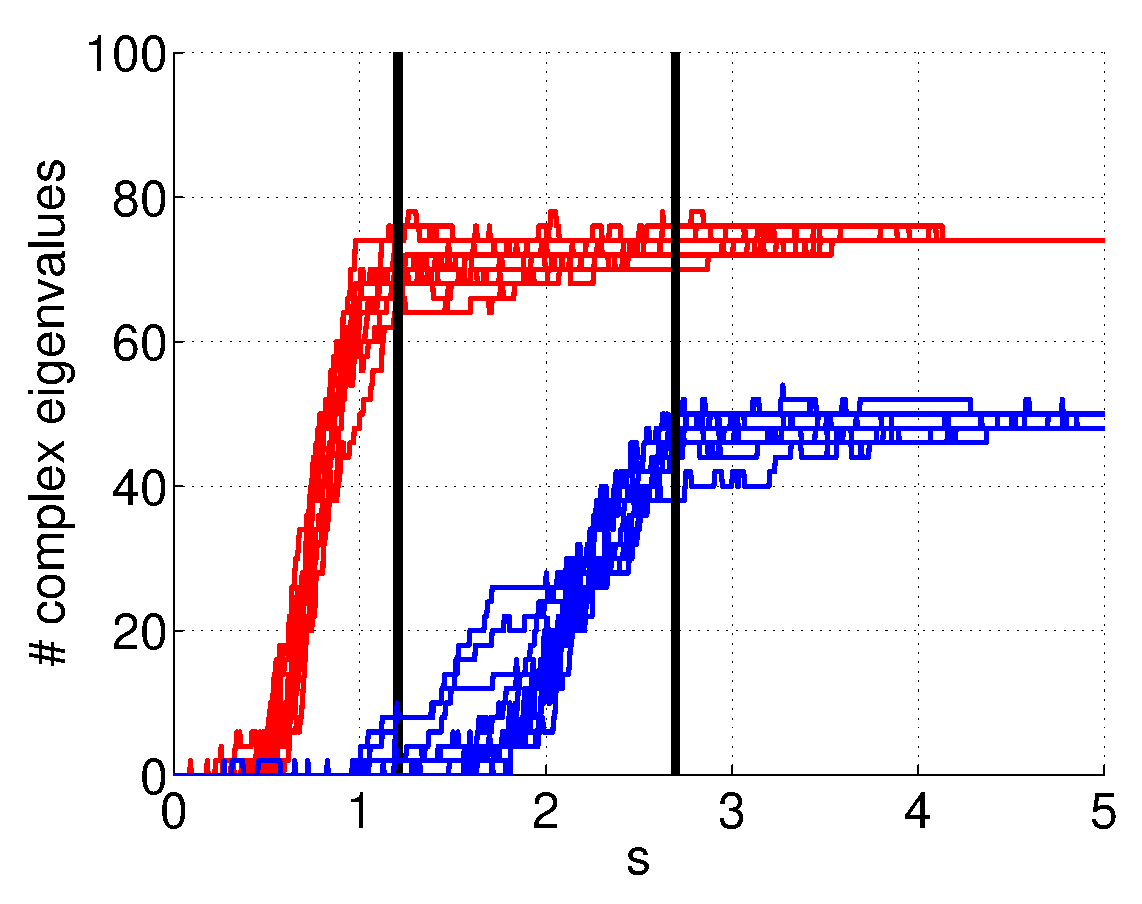
\includegraphics[height=5cm]{/Figs/num_cplx.eps}
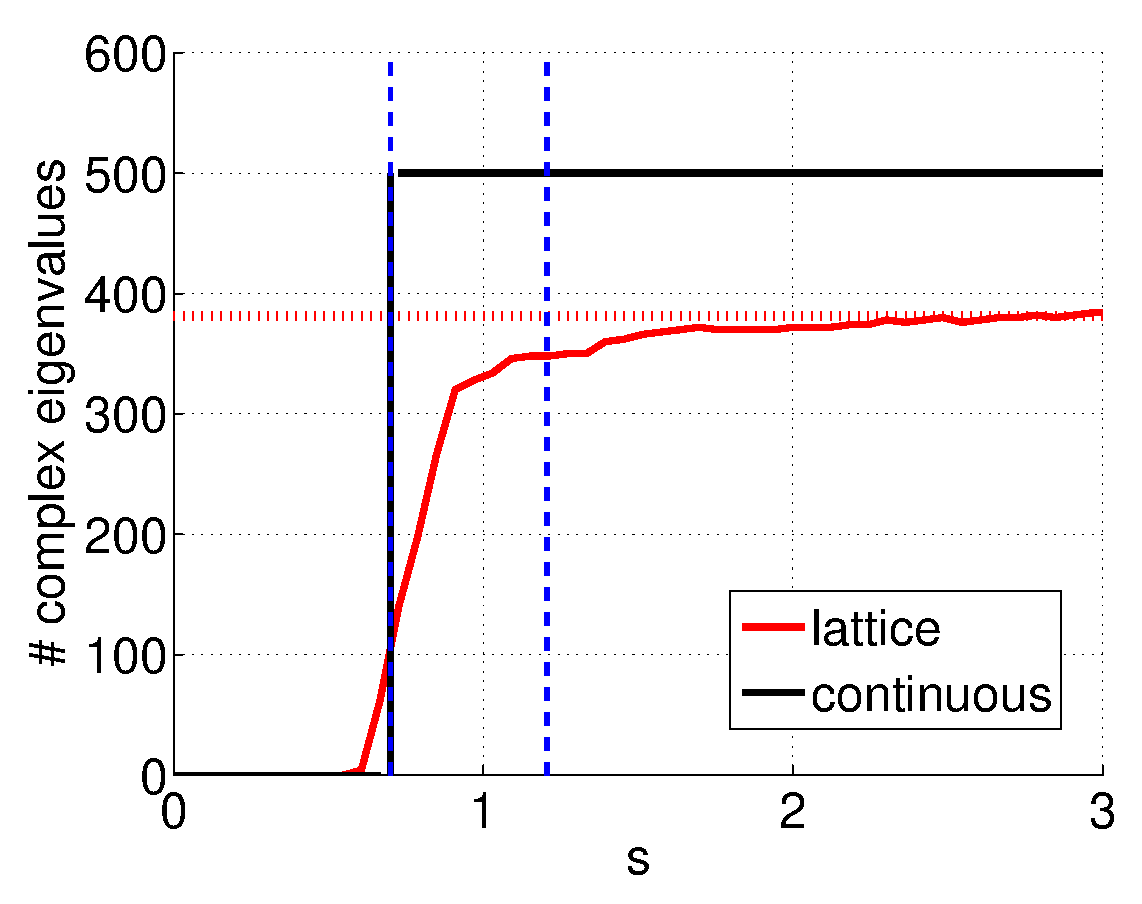
\includegraphics[height=5cm]{/Figs/numComplex_500}
\caption{Left: Number of complex eigenvalues vs. $s$ for $N=100$ sites. Each red line corresponds to a different 
realisation of field disorder with $\sigma=3$(red) and $\sigma=5$ (blue), but $\Delta=0$. The black vertical lines are at values of $s$ at which the sliding transition occurs.
Right: Number of complex eigenvalues vs. $s$ for $N=500$ sites and $\sigma=5$ (red)
vs. the result of the continuous problem(black step function)
The vertical dashed lines are $s_{1/2}$ and $s_1$. The dotted horizontal red line is the estimated saturation value, \Eq{e101}.}
\label{figCplxSat}
\end{figure}

If we look at the gap, then it becomes complex at $s_{1/2}$ and has a peak at $s_{1}$.
If there is off diagonal disorder, then the peak is diminished. 
%
We would like to establish wether there is a finite gap in the spectrum and how it scales with the system size $N$.
The gap $\Delta$ in the spectrum is just the real part of the second largest eigenvalue.
Our goal is to characterise the gap for the general disordered hopping model, see for example \Fig{fig11}.
At $s=s_{1/2}$ the gap becomes complex and at $s=s_{1}$ the gap reaches a peak value. 
It is easy to explain the large $s$ behavior - which is just the clean ring limit. 
Recall (\Eq{e23}, \Eq{e24}) that for a clean ring the eigevalues are $\lambda_n \propto (n/N)^2$,
hence $\Delta = \lambda_1 \sim 1/N^2$
and  the integrated density of states $\mathcal{N}(\lambda) \propto N \lambda^{1/2}$.
%
\rmrk{Near the peak it can be shown that $\mathcal{N}(\lambda)\propto N \lambda$, leading to $\Delta\sim 1/N$.}

%%%%%%%%
%\begin{figure}[h]
%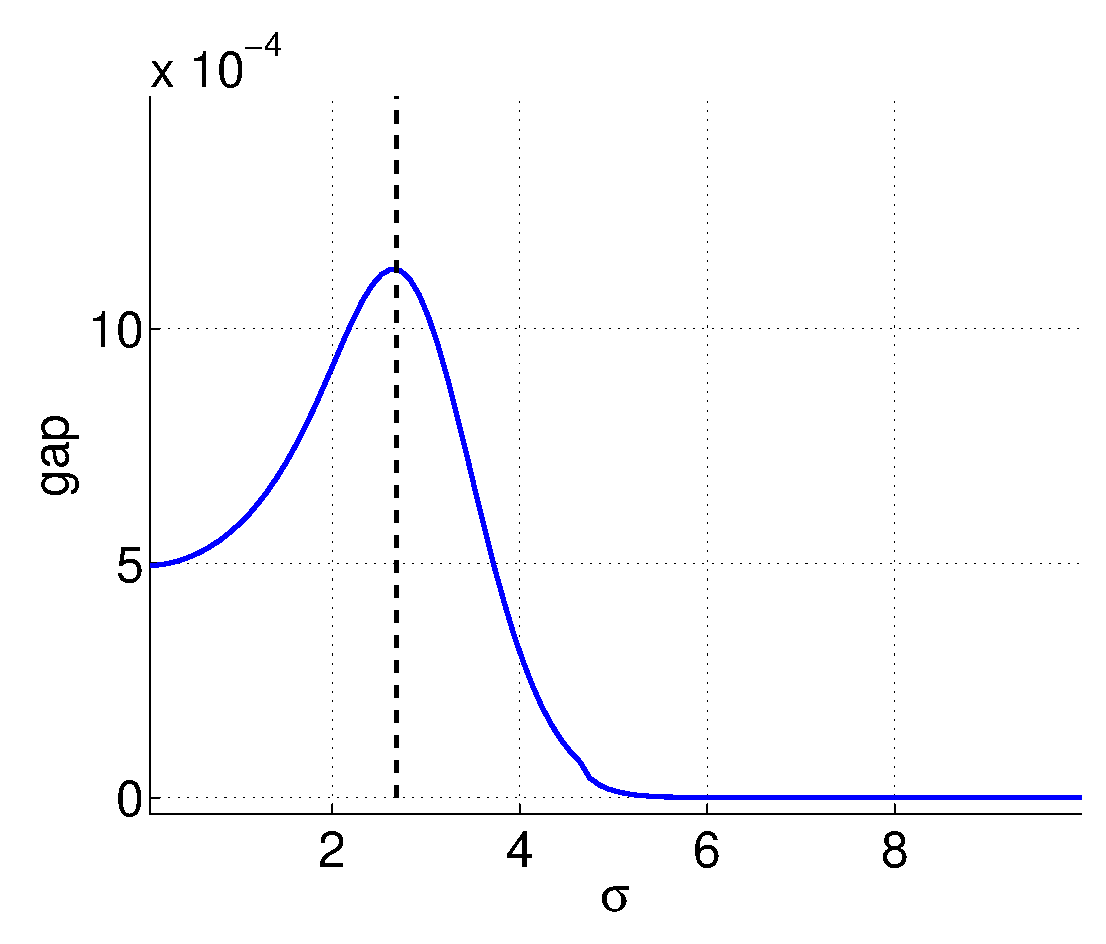
\includegraphics[height=5cm]{/Figs/gap_sigma.eps}
%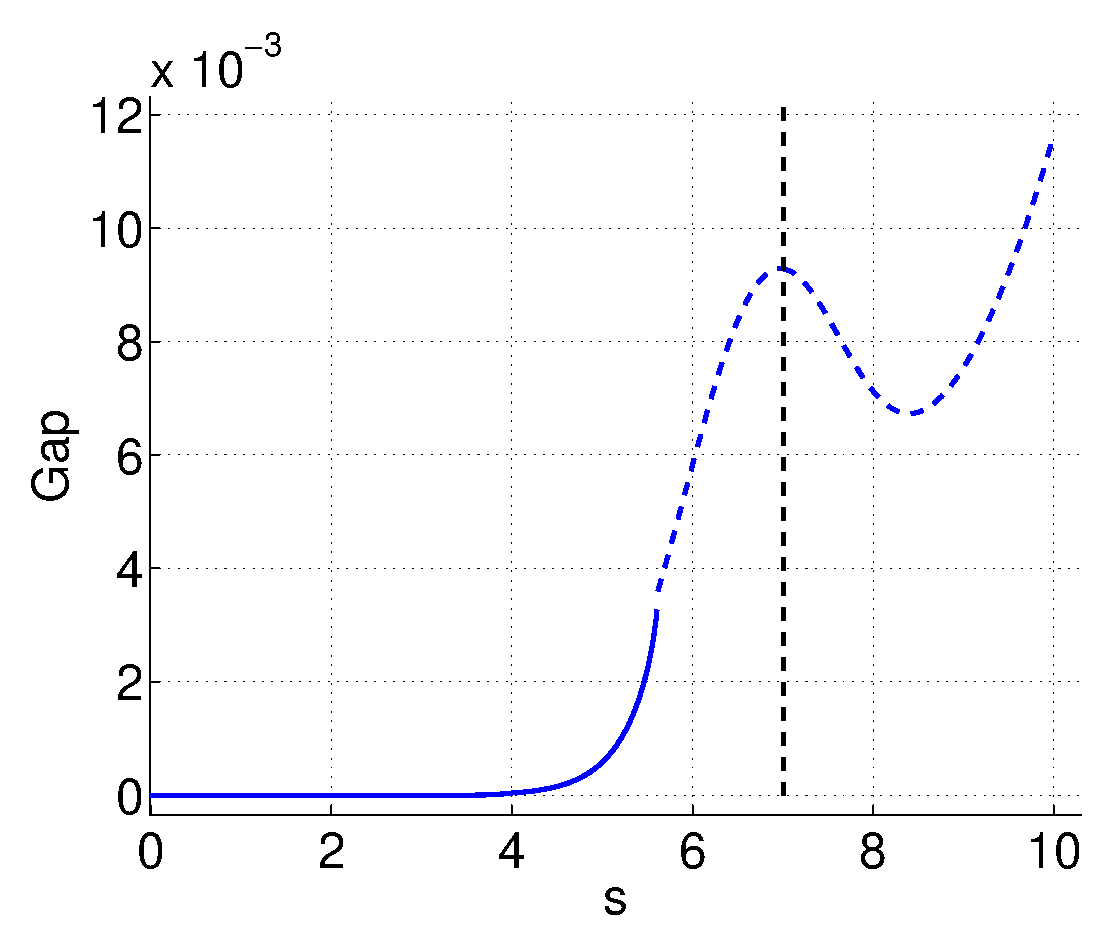
\includegraphics[height=5cm]{/Figs/gap_s_sigma_10.eps}
%\caption{
%Left panel: The gap in the spectrum vs. the field disorder $\sigma$ (left panel) for fixed $s$. 
%At $\sigma=\sigma_c$ the gap begins to close exponentially in $\sigma$. The value $\sigma_c=2.69$ (dashed black line) is determined by the Derrida transition. Here $N=300$ and $s=1$.
%Right panel: the gap in the spectrum vs. $s$.
%At $s=s_c$ (dashed black line)  the gap begins to close. This point is determined by the Derrida transition. Here $N=300$ and $\sigma=10$. Dashed lines indicate that the gap is complex.}
%\label{fig11}
%\end{figure}


%%%%%%%%
\begin{figure}[h]
%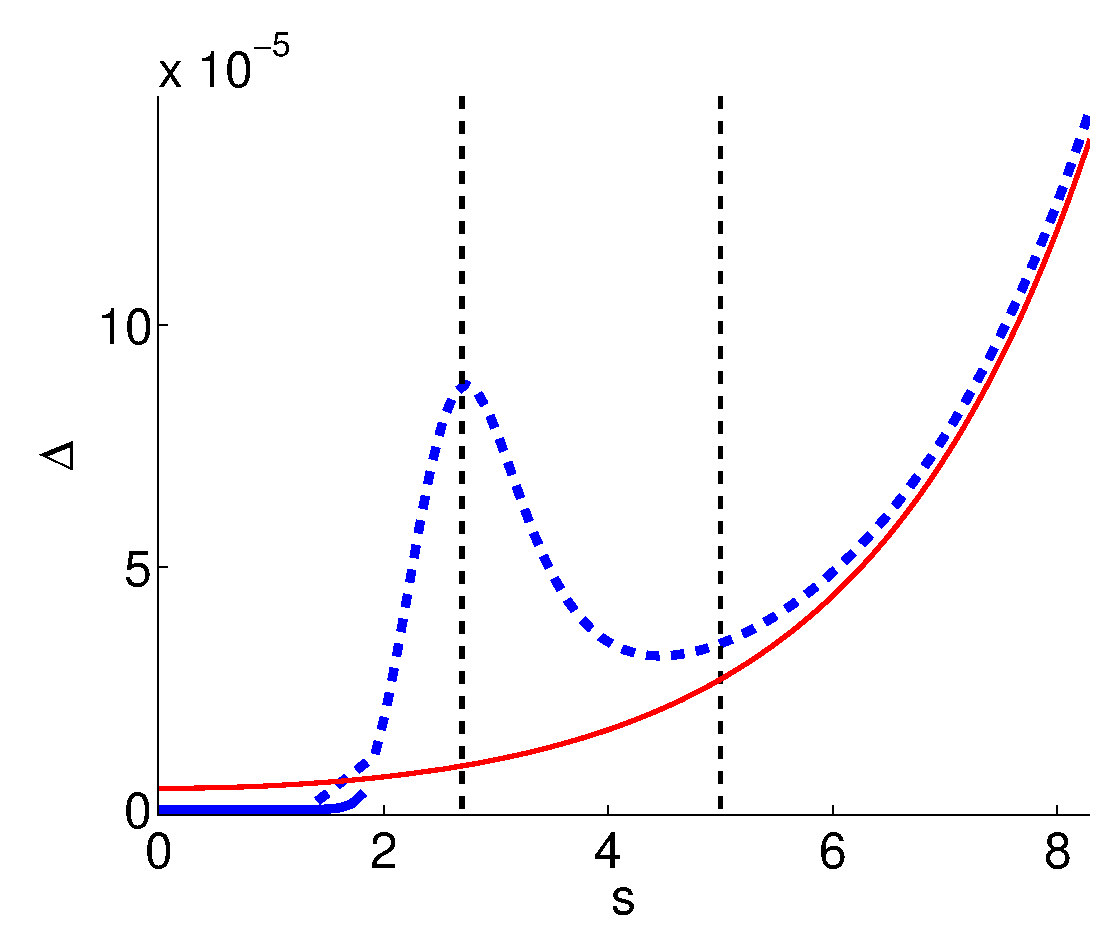
\includegraphics[height=5cm]{/Figs/gap_vs_s_disorder.eps}
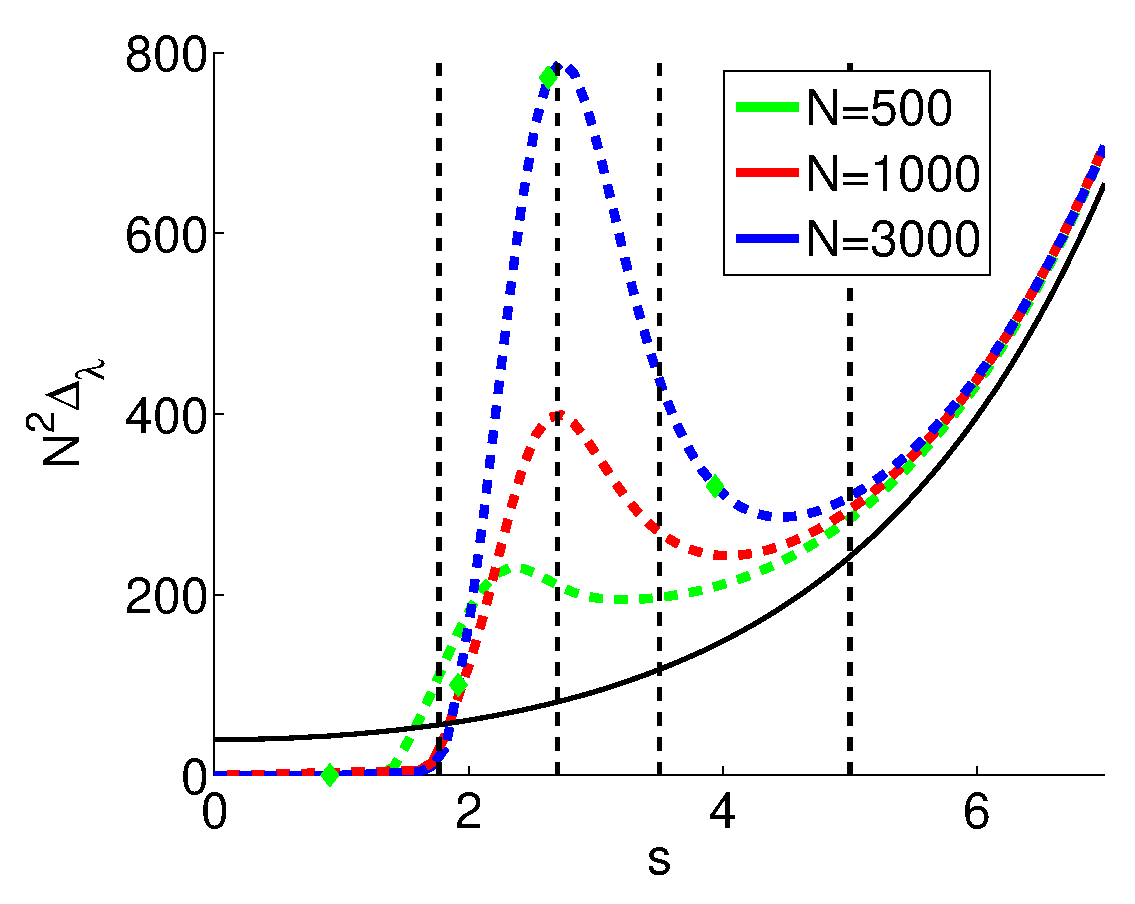
\includegraphics[height=5cm]{/Figs/gap_s_N2.eps}
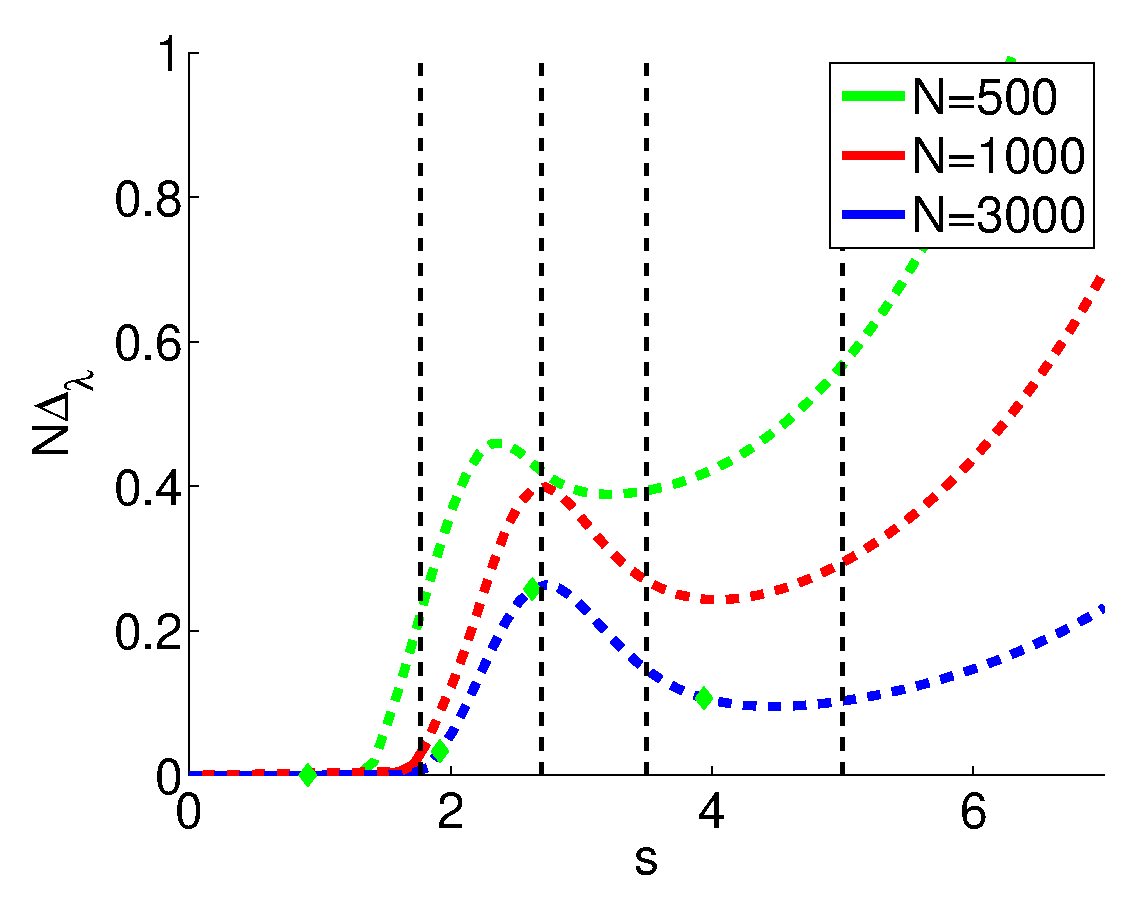
\includegraphics[height=5cm]{/Figs/gap_s_N.eps}

\includegraphics[height=5cm]{/Figs/gap_delta_3000.eps}
\caption{
Top row: Gap vs. $s$ with disorder $\sigma=5$. The dashed segment corresponds to a complex spectrum. The three lines corresponds to different values of $N$. 
The black line is $4\pi^2/N^2 \cosh(s/2)$, as in a clean ring. 
The vertical dashed lines are $s=s_{1/2}, \ s_1, \ s_2$ and $s=s_{\infty}=\sigma$.
On the left the gap is rescaled by $N^2$, on the right by $N$, showing that near the peak
$\Delta_{\lambda} \sim 1/N$ and for $s>s_{\infty}$, $\Delta_{\lambda} \sim 1/N^2$. 
Bottom panel: The gap vs. $s$ for different values of off diagonal disorder, $\Delta$, illustrating that 
the off diagonal disorder, or "glassiness" kills the gap.}
\label{fig11}
\end{figure}
%%%%%%%%%%%%%%%%%%%%

%%%%%%%%%%%%%%%%%%%%%%%%%%%%%%%%%%%%%%%%%%%%
\subsect{Scaled affinity, cumulants of the stochastic field}

For stochastic fields that have a uniform distribution with width $\sigma$, \Eq{e2} becomes 
%
\beq
s_{\mu} = \frac{1}{\mu}\ln\left(\frac{\sinh(\mu\sigma)}{\mu\sigma}\right)
\eeq
%
where $s_{\mu}$ is the scaled affinity. It is interesting that for large $\mu$, it saturates 
and $s_{\infty} = \sigma$.
In contrast, if the stochastic field has a normal distribution with standard deviation $\sigma$, then 
$s_{\mu}=(1/2)\sigma^2 \mu$ and the scaled affinity is unbounded. 
The two models agree only for  small $\mu$ (see \Fig{s_mu}).  Note that $\text{var[box]}=\sigma^2/12$ and $\text{var[normal]}=\sigma^2$.

%%%%%%%%%%%%%%%%%%%%%%%%%%%%%%%%%
\begin{figure}[h]
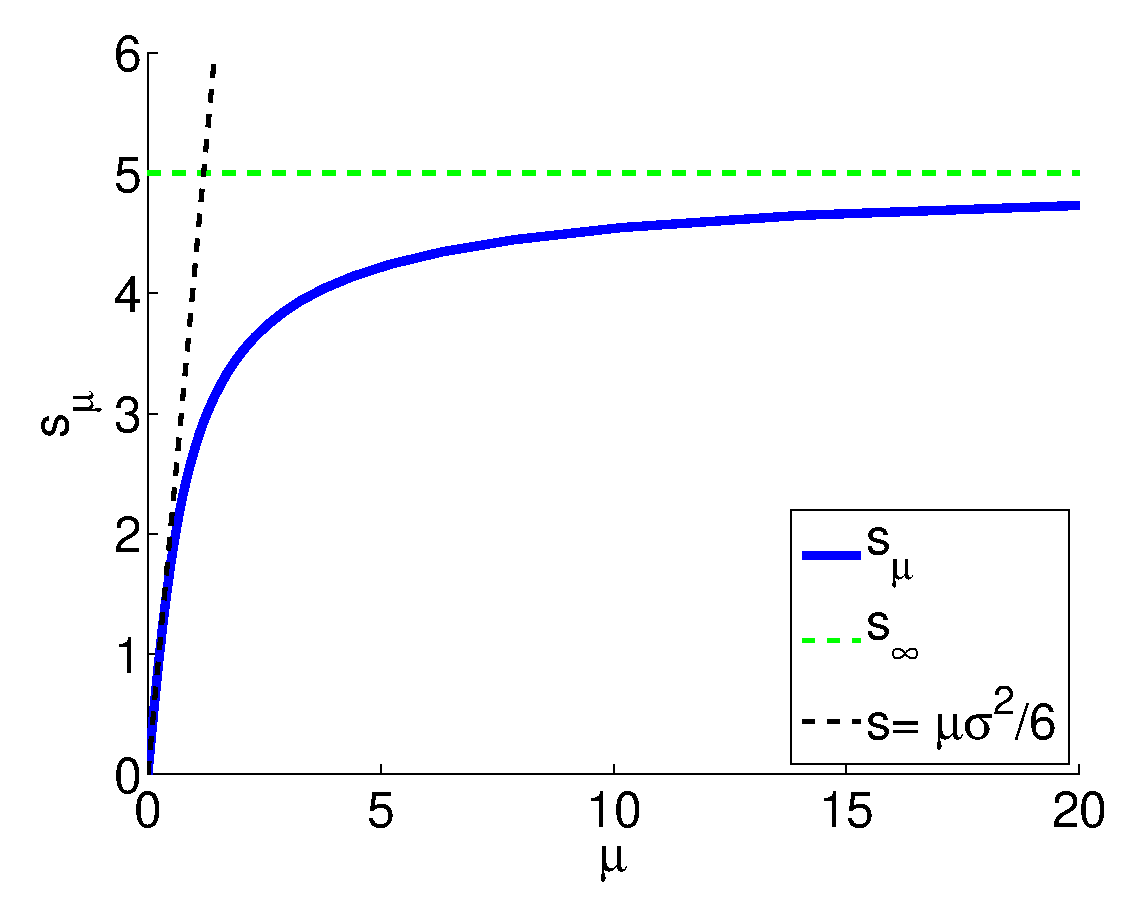
\includegraphics[height=5cm]{/Figs/s_mu.eps}
\caption{
The scaled affinity $s_{\mu}$ saturates at $s \ = \ s_{\infty} \ = \ \sigma$.
}
\label{s_mu}
\end{figure}


\subsect{Algorithm for analysis}

Given an asymmetric and conservative matrix
%
\beq
W \ =\  -\text{diag}[\Gamma_{n-1}] + \text{offdiag}[ g_n e^{\pm (s + \sigma_n)/2 }]
\eeq
%
The diagonal elements (decay rates) are determined by the conservativity requirement
%
\beq
\Gamma_n (s)&=& g_{n-1}e^{-(s+\sigma_{n-1})/2} + g_{n} e^{(s+\sigma_n)/2}
\eeq 
%
we take the following steps
\begin{enumerate}
\item Gauge away the field disorder, we are left with an asymmetric matrix of the form
%
\beq
e^{V/2}We^{-V/2} \ = \  \tilde{W} = -\text{diag}[\Gamma_{n-1}(s)] + \text{offdiag}[ g_n e^{\pm s/2}]
\eeq 
%
where the diagonal depends on $s, \sigma$ and $\Delta$. 
Note that the some of each column of the gauged matrix is not zero.

%
\item Define the associated hermitian matrix by setting $s=0$ on the off diagonal. 
Now we have the matrix 
%
\beq
H = -\text{diag}[\Gamma_{n-1} (s)] + \text{offdiag}[ g_n ]
\eeq 
%
which is {\em symmetric and non conservative}. Note that the diagonal elements depend on $s$!
%
\item Calculate the eigenvalues of the associated Hermitian matrix, $\varepsilon_j (s)$.
\item The eigenvalues of the original, non hermitian problem are solutions to the secular equation 
%
\beq
\prod_{j=1}^N \left(\lambda - \varepsilon_j(s)\right)  \ = \ 
\left[\prod_{n=1}^N g_n\right]  2\left(\cosh\left(\frac{sN}{2}\right) -1\right)
\eeq
%
where $\lambda$ is complex.

\item
According to Thouless, the left hand side of the equation can be written as 
%
\beq
e^{N/\xi} = \prod_{j=1}^N \left(\lambda - \varepsilon_j(s)\right) 
\eeq
%
where the inverse localization length
%
\beq
\kappa \equiv \xi^{-1}  = \frac{1}{N} \sum_{j=1}^N \ln\left(\left| \lambda - \varepsilon_j(s) \right| \right)
\eeq
%
is equivalent to a 2D electrostatic potential due to charges $q_j = \varepsilon_j(s)$ along the $x$ axis.
Once we determine the density of states, we can solve the electrostatic problem.
This will allow us to determine when the eigenvalues are complex and wether there is a finite gap.

\item For weak disorder, the inverse localization length of the lower bands of the associated hermitian system can be calculated by FGR.
%

%
\end{enumerate}

%%%%%%%%%%%%%%%%%%%%%%
\subsect{Electrostatic analogy}
%

According to Thouless, the inverse localization length $\kappa$ is given by 
%
\beq
\kappa(\lambda) &=& \frac{1}{N} \sum_{j=1}^N \ln\left(\left| \lambda - \varepsilon_j(s) \right| \right)
\eeq
%
The inverse localization length is in fact the sum of point charges on a line in 2 dimensions. 
In the limit $N\to\infty$, the sum is replaced by an integral and $\kappa$ can be expressed as an 
electrostatic potential. Using the notation $\lambda = z = x+iy$ and $\varepsilon_j = x'$,
%
\beq
\Phi = \varphi(x,y) + i \psi(x,y) = \int \ln \left( z - x'\right) \rho(x') dx' 
\eeq
%
The real part is the electrostatic potential $\kappa \ = \ \varphi(x,y)$
%
\be{65}
\varphi(x,y) = \int \ln \left(|z-x'|\right) \rho(x')dx' =\frac{1}{2} \int \ln \left[(x-x')^2 + y^2\right] \rho(x')dx' 
\ee
%
The imaginary part is the field lines
%
\beq
\psi(x,y) = \arg (z-x')
\eeq
%
The non hermitian requirement that
\beq
\varphi(x)=\ln\left[2(\cosh\left(\frac{sN}{2}\right) -1)\right]
\eeq
defines an equipotential line. \\
The requirement 
%
\beq
\psi(x,y) = 2\pi n, \ n=0,\pm1,\pm2,...
\eeq
%
defines the field lines, that are perpendicular to the equipotential lines (this is a result of the Cauchy-Riemann equation).
To determine the gap we need the intersection of the equipotential line with the field line
that originates from the first point charge (lowest eigenvalue of the associated Hermitian problem).

%%%%%%%%%%%%%%%%%%%%%%%%%%%%%%%%%
\subsect{The Density of states of the associated Hermitian matrix}

For weak disorder, $\mathcal{S} \gg \sigma$, 
the diagonal elements of the associated Hermitian matrix are large compared to the off-diagonal elements, $\gamma_n\gg1$.
Also, in this limit the diagonal elements are uncorrelated. As a result, their distribution is just a log-box distribution, i.e.
%
\beq
\rho(\varepsilon) = \frac{1}{\sigma \varepsilon},  \ \ \sigma = \ln \frac{\varepsilon_{\max}}{\varepsilon_{\min}}
\eeq
%
For strong disorder,  $\mathcal{S} \ll \sigma$, the coupling terms cannot be neglected and also the decay rates are correlated. It has been shown \cite{odh3} that for this kind of problem
the density of states exhibits a "spectral condensate" at 
$\varepsilon=0$ and not a "Lifshitz tail", See \Fig{DOS}. 

%
\begin{figure}[h]
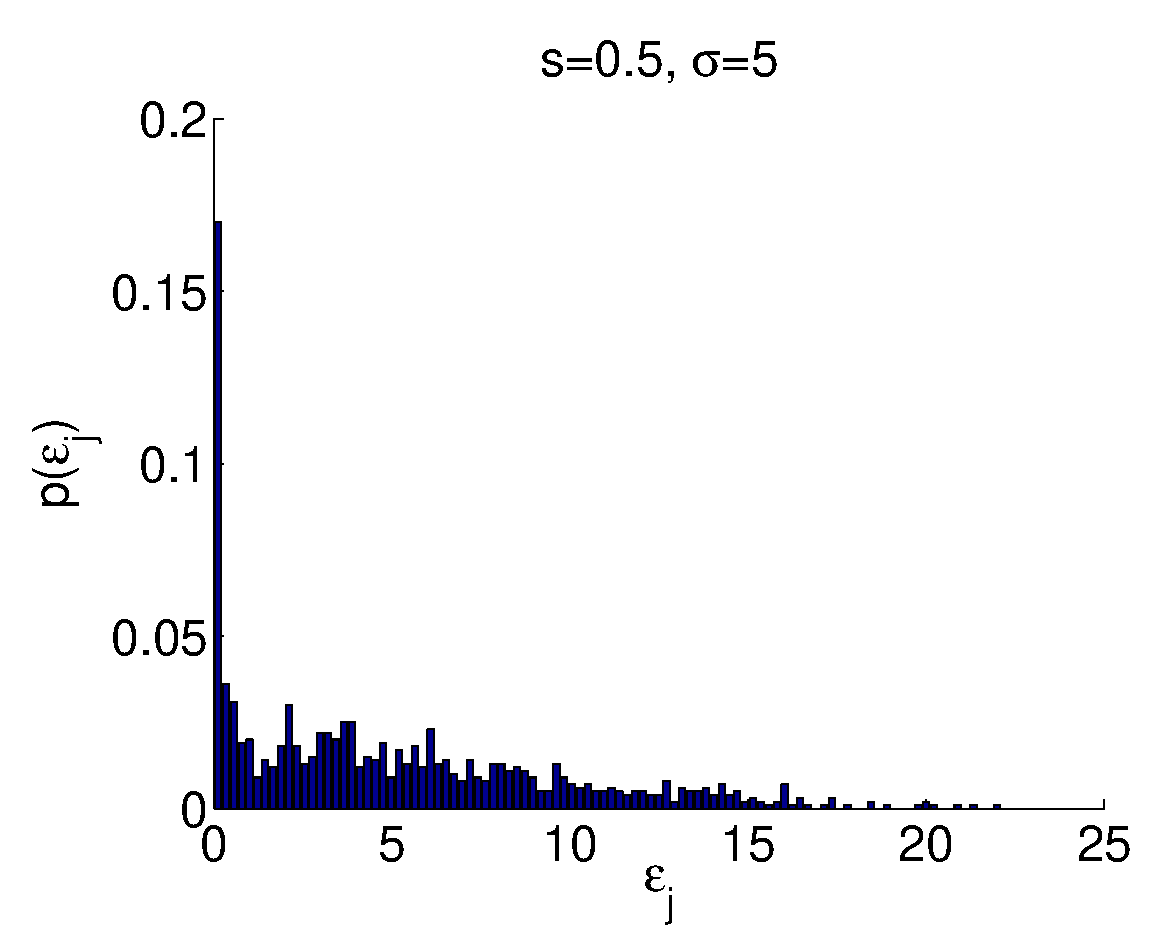
\includegraphics[height=4.5cm]{/Figs/P_eps_strong.eps}
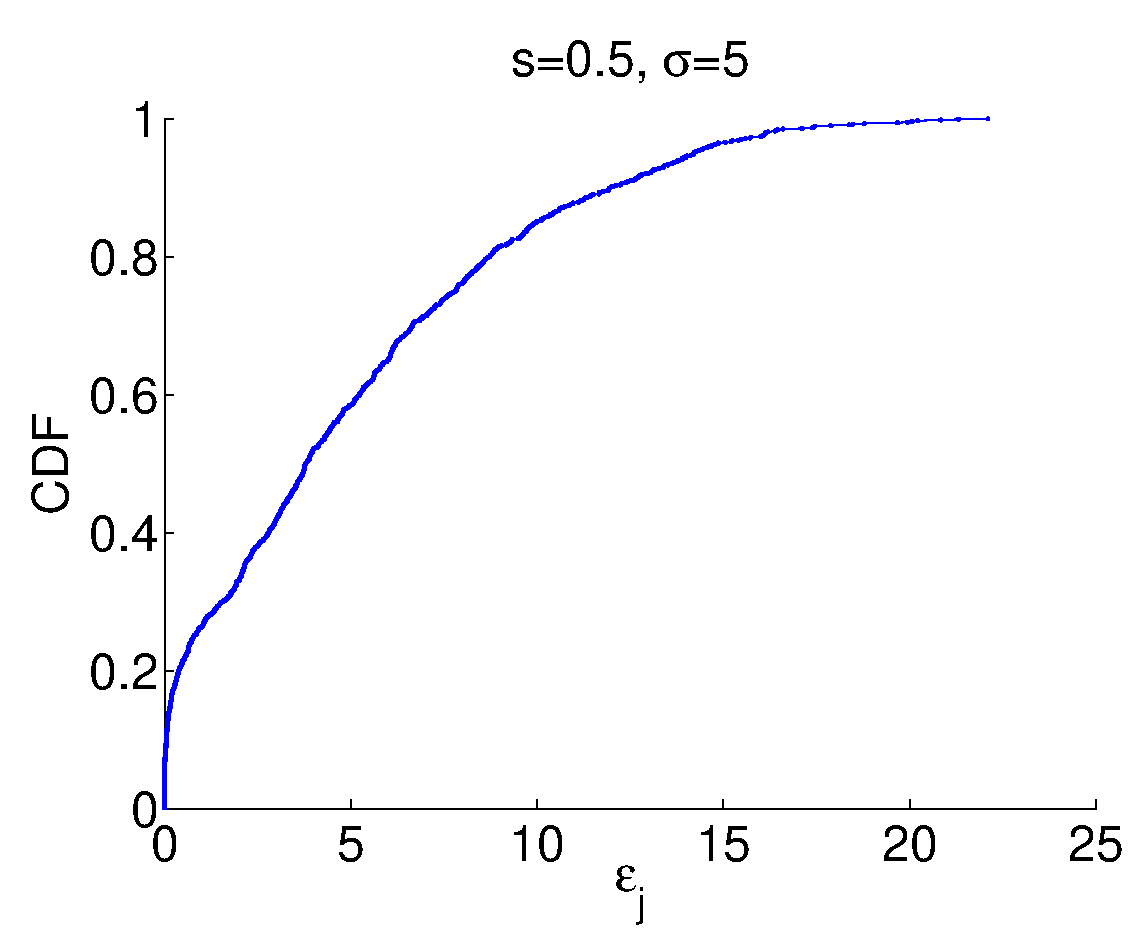
\includegraphics[height=4.5cm]{/Figs/CDF_eps_strong.eps}
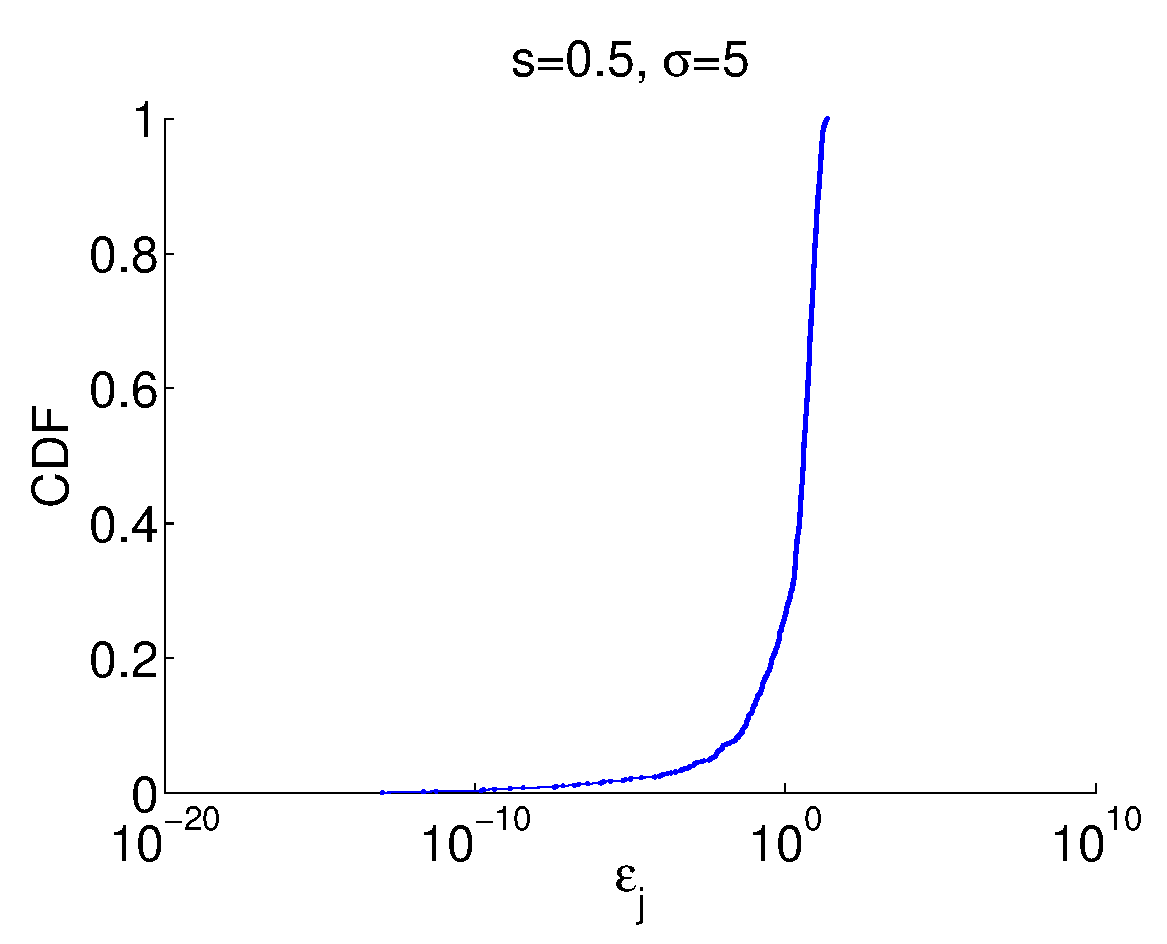
\includegraphics[height=4.5cm]{/Figs/CDF_log_eps_strong.eps}

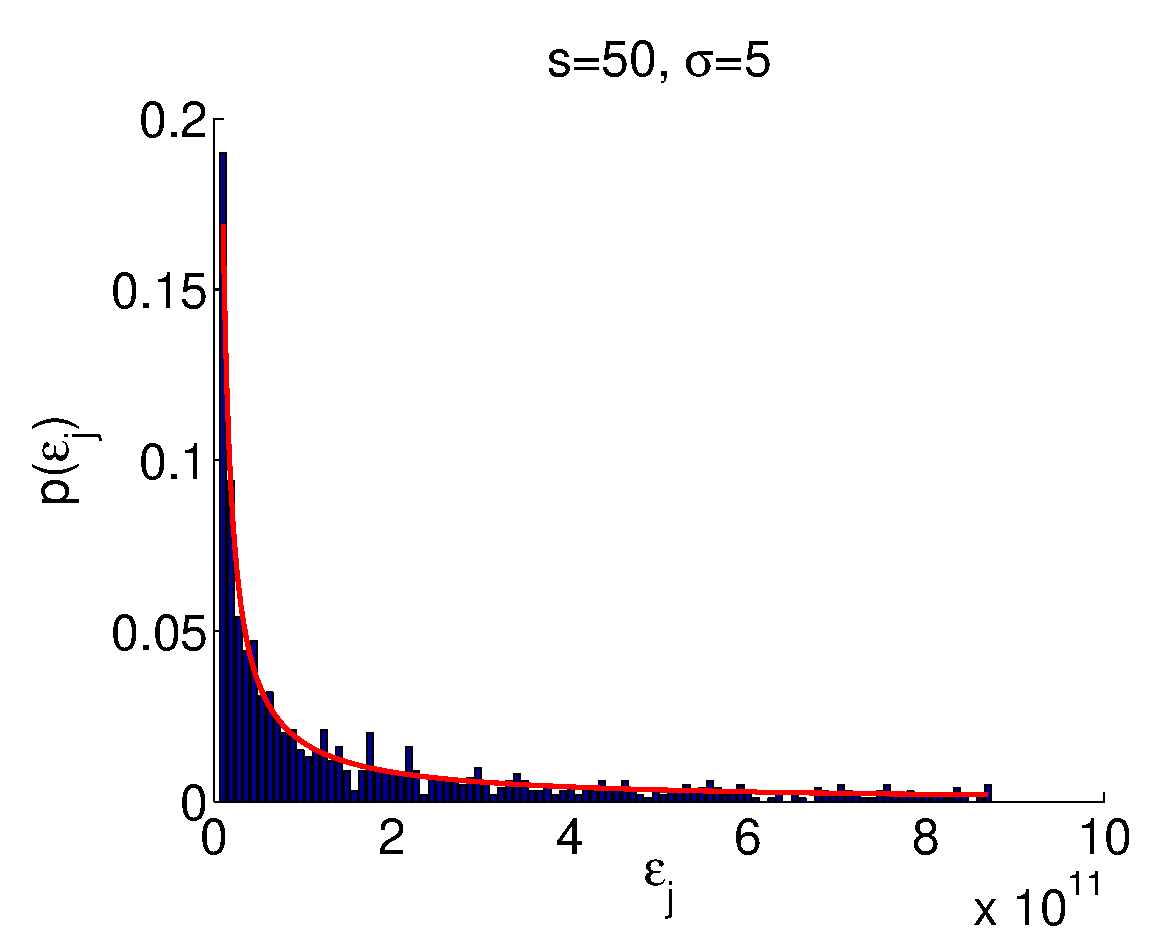
\includegraphics[height=4.5cm]{/Figs/P_eps_weak.eps}
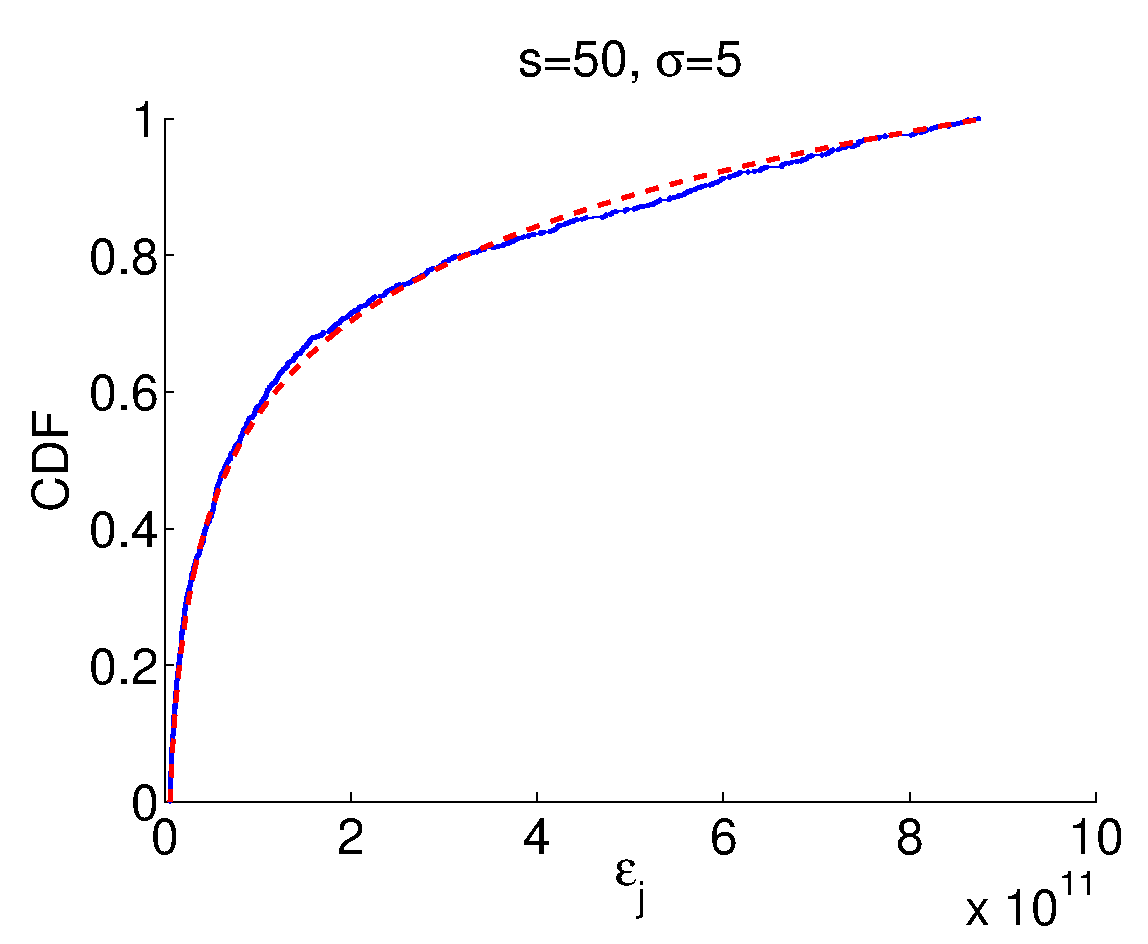
\includegraphics[height=4.5cm]{/Figs/CDF_eps_weak.eps}
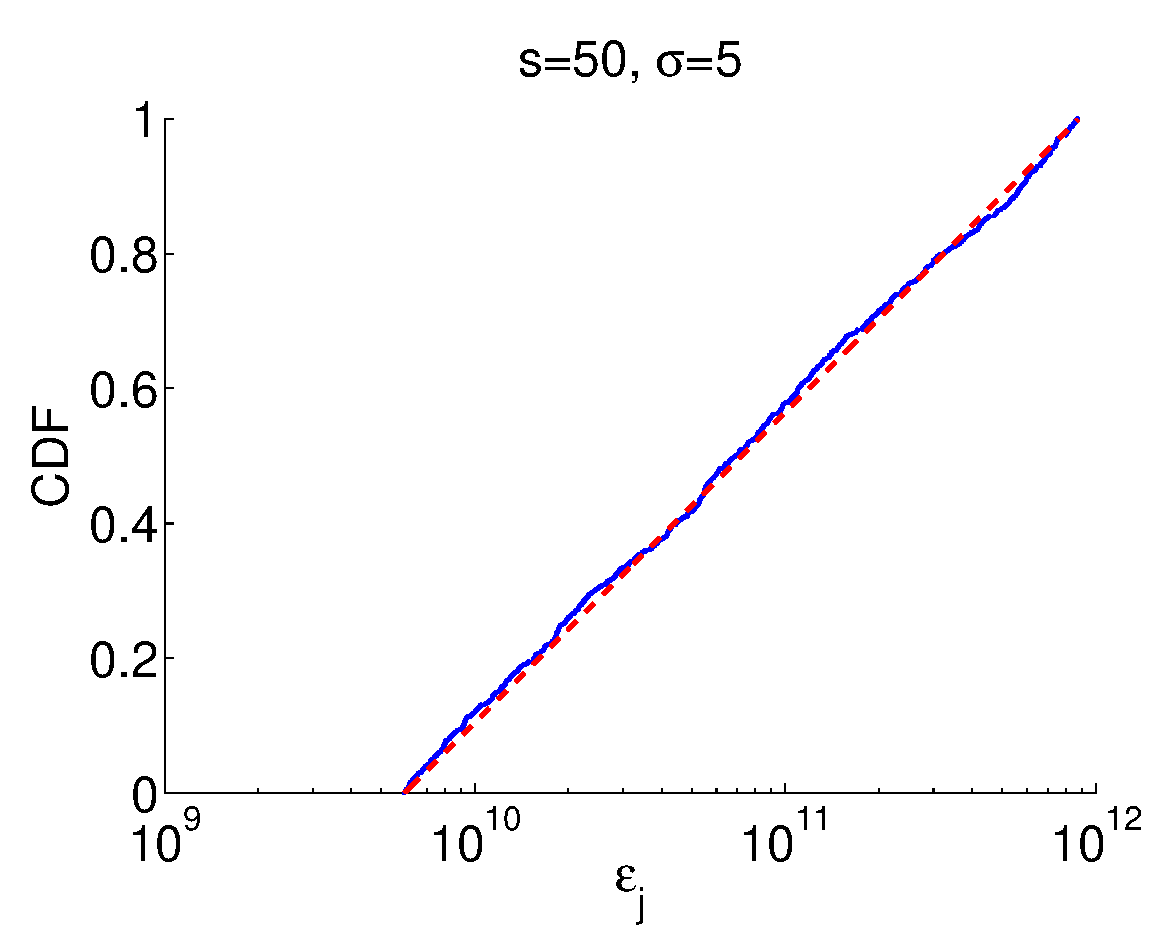
\includegraphics[height=4.5cm]{/Figs/CDF_log_eps_weak.eps}

\caption{
Top row: Histogram and cumulative distribution function for strong disorder ($\mathcal{S}\ll\sigma$).
Bottom row: Histogram and cumulative distribution function for weak disorder ($\mathcal{S}\gg\sigma$), the 
density of states is $\rho = (\sigma x)^{-1}$ (solid red line).
The right hand column is the CDF of $\log(\varepsilon_j)$ to highlight the lower tail.
The simulation is for $N=1000$ sites, $\sigma=5$ and $\mathcal{S}=0.5, 50$.
}
\label{DOS}
\end{figure}
%
\begin{figure}[h]
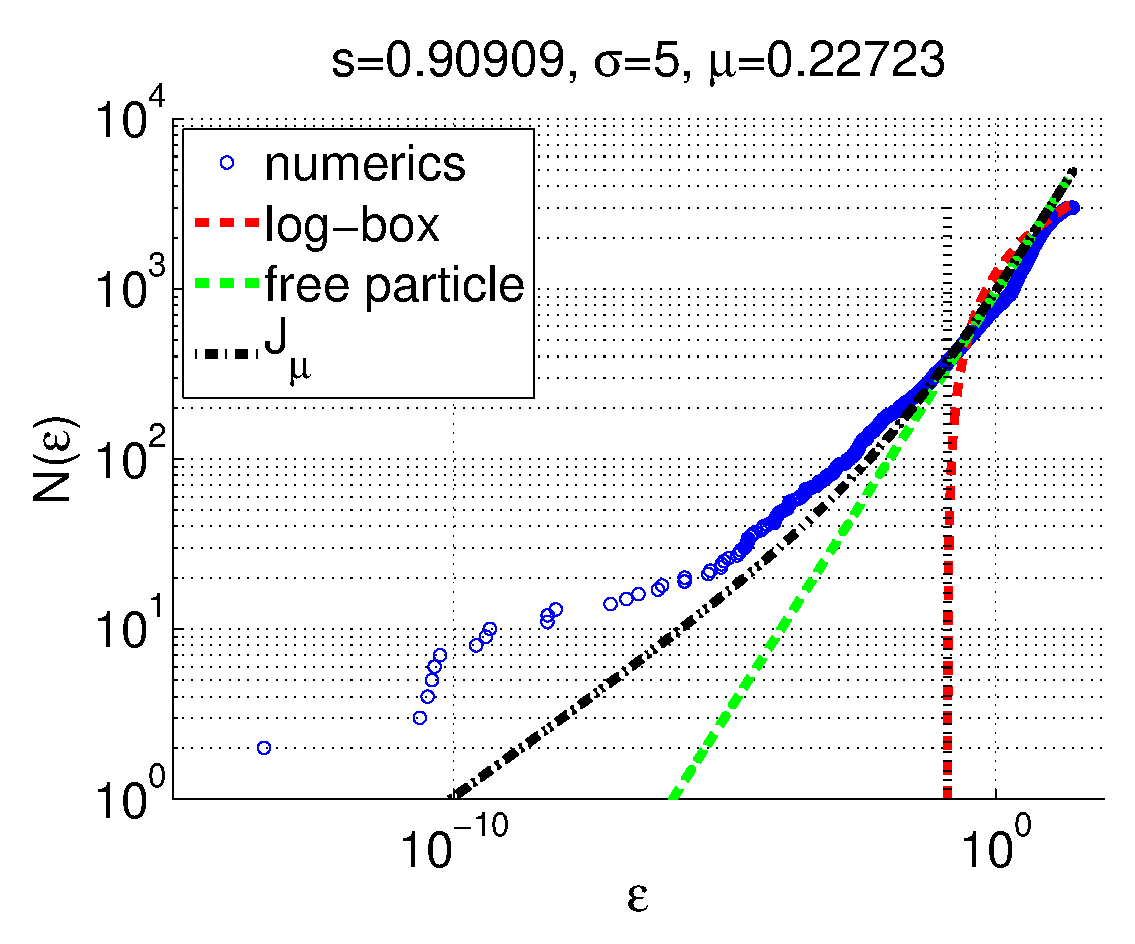
\includegraphics[height=4.5cm]{/Figs/NumStates_10}
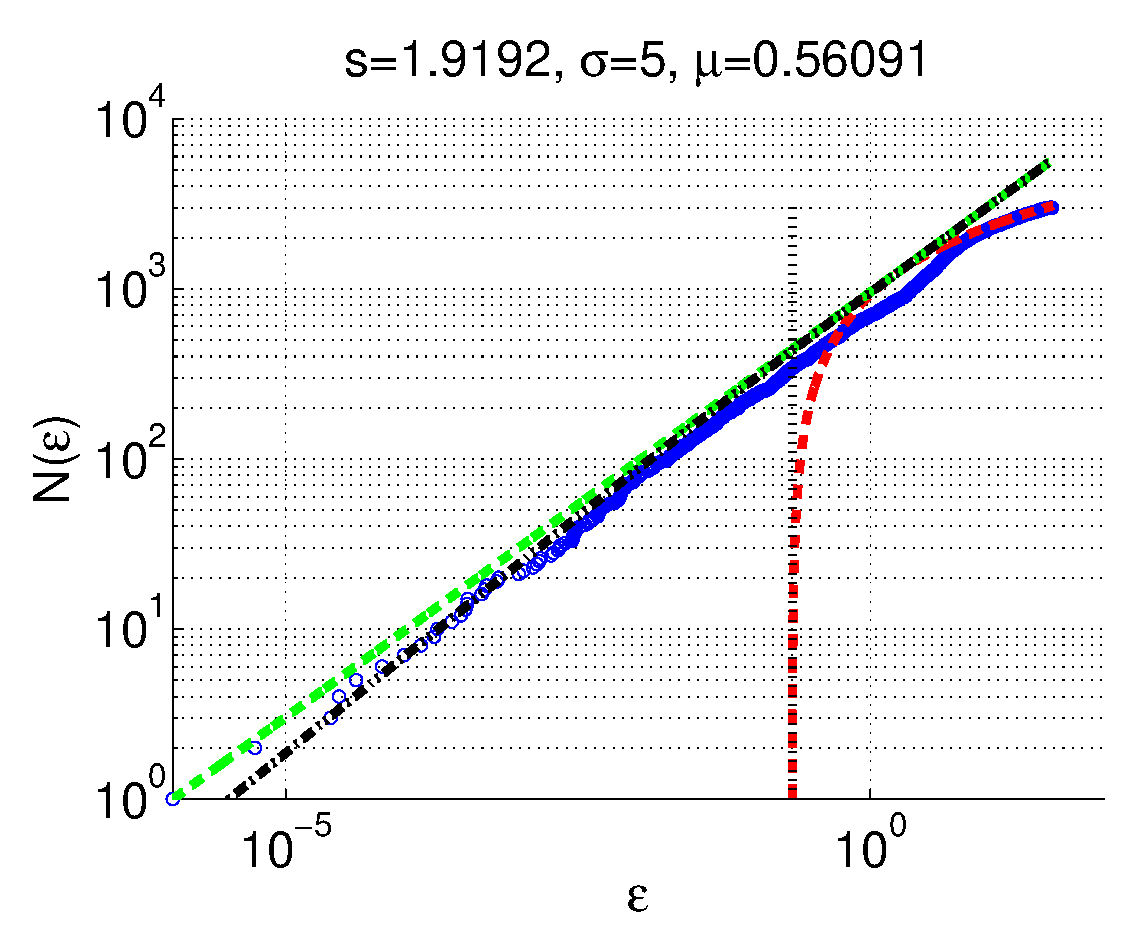
\includegraphics[height=4.5cm]{/Figs/NumStates_20}
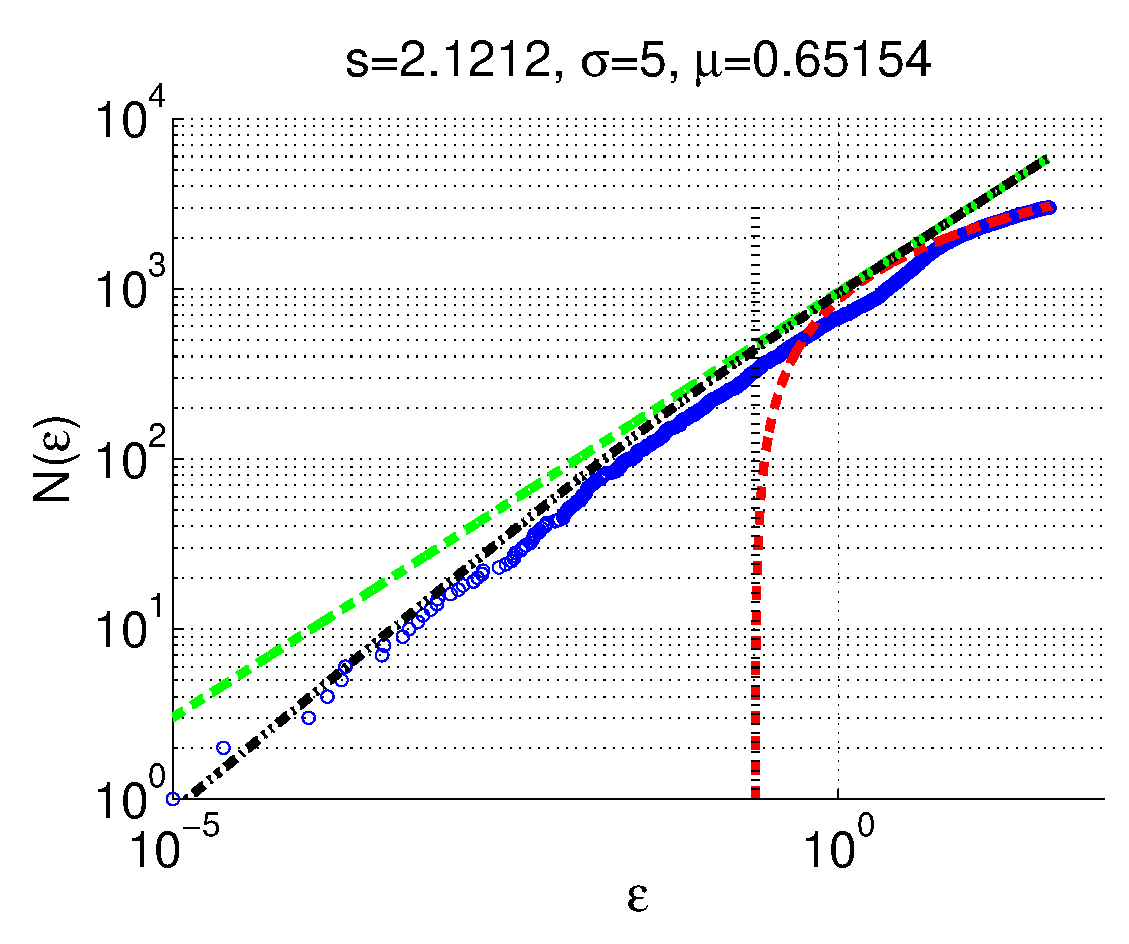
\includegraphics[height=4.5cm]{/Figs/NumStates_22}
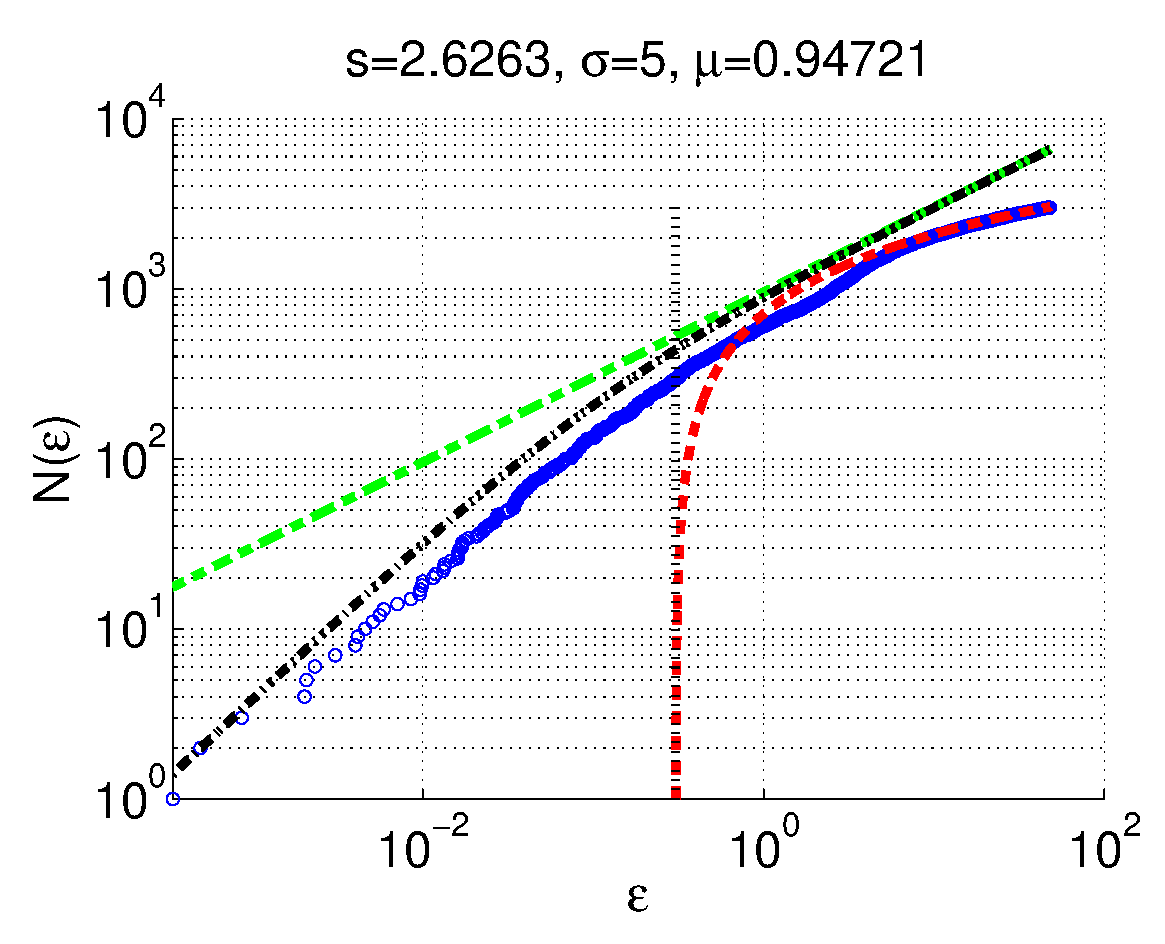
\includegraphics[height=4.5cm]{/Figs/NumStates_27}
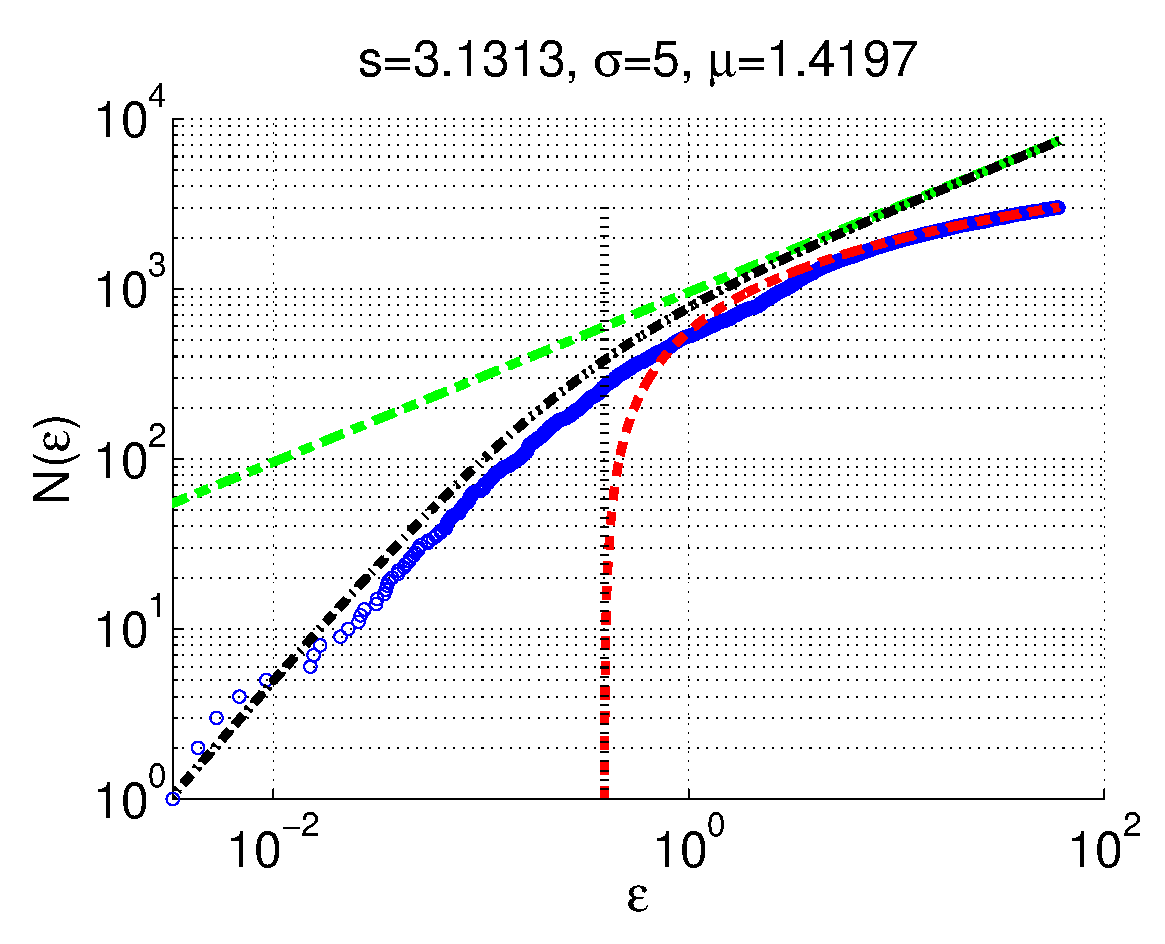
\includegraphics[height=4.5cm]{/Figs/NumStates_32}
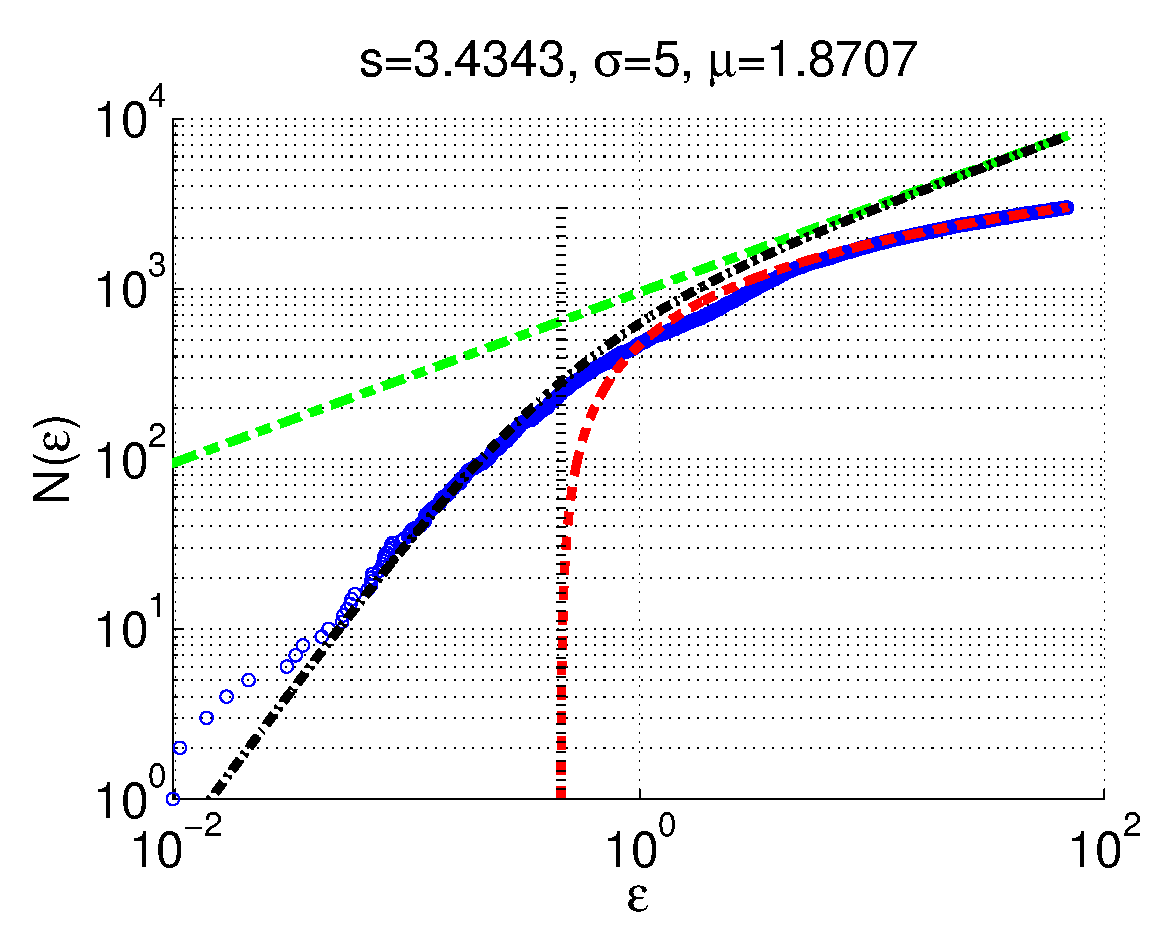
\includegraphics[height=4.5cm]{/Figs/NumStates_35}
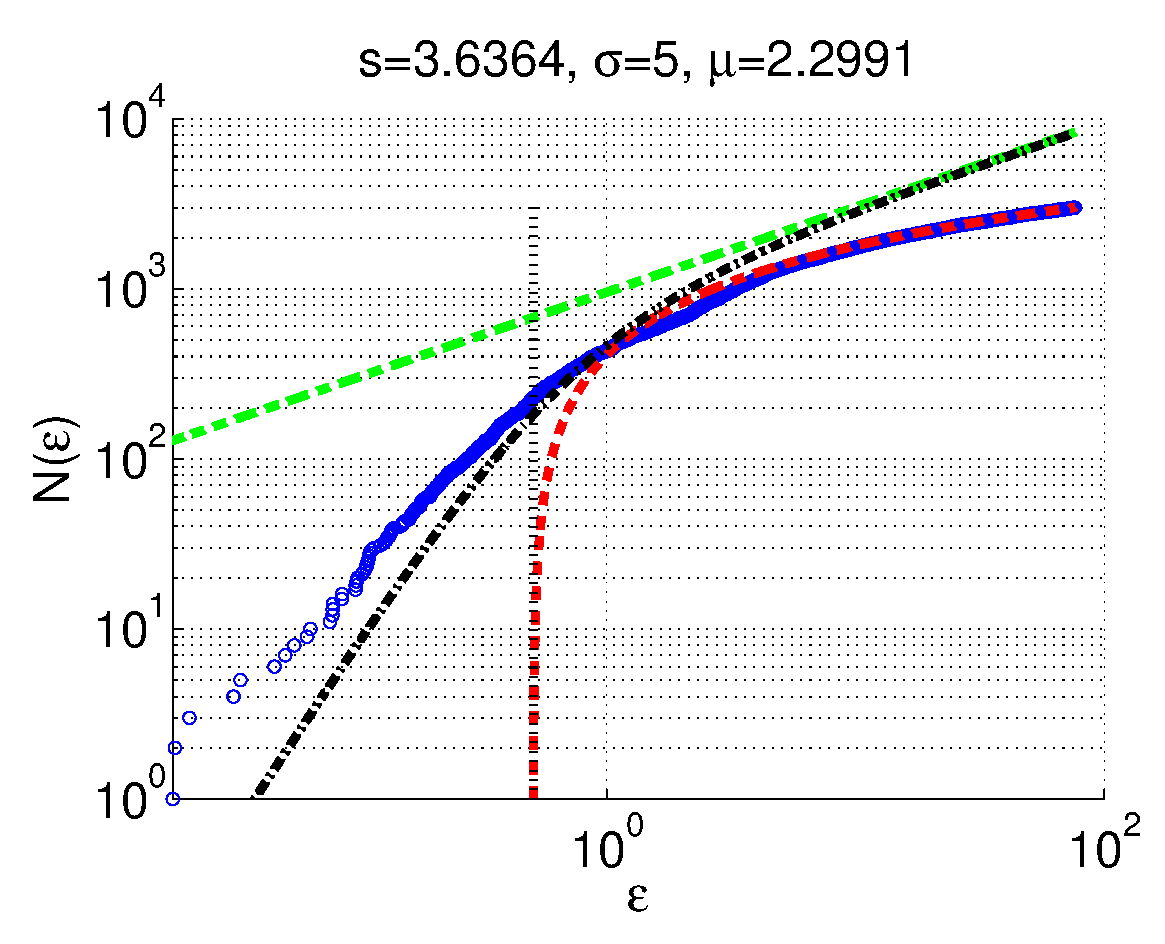
\includegraphics[height=4.5cm]{/Figs/NumStates_37}
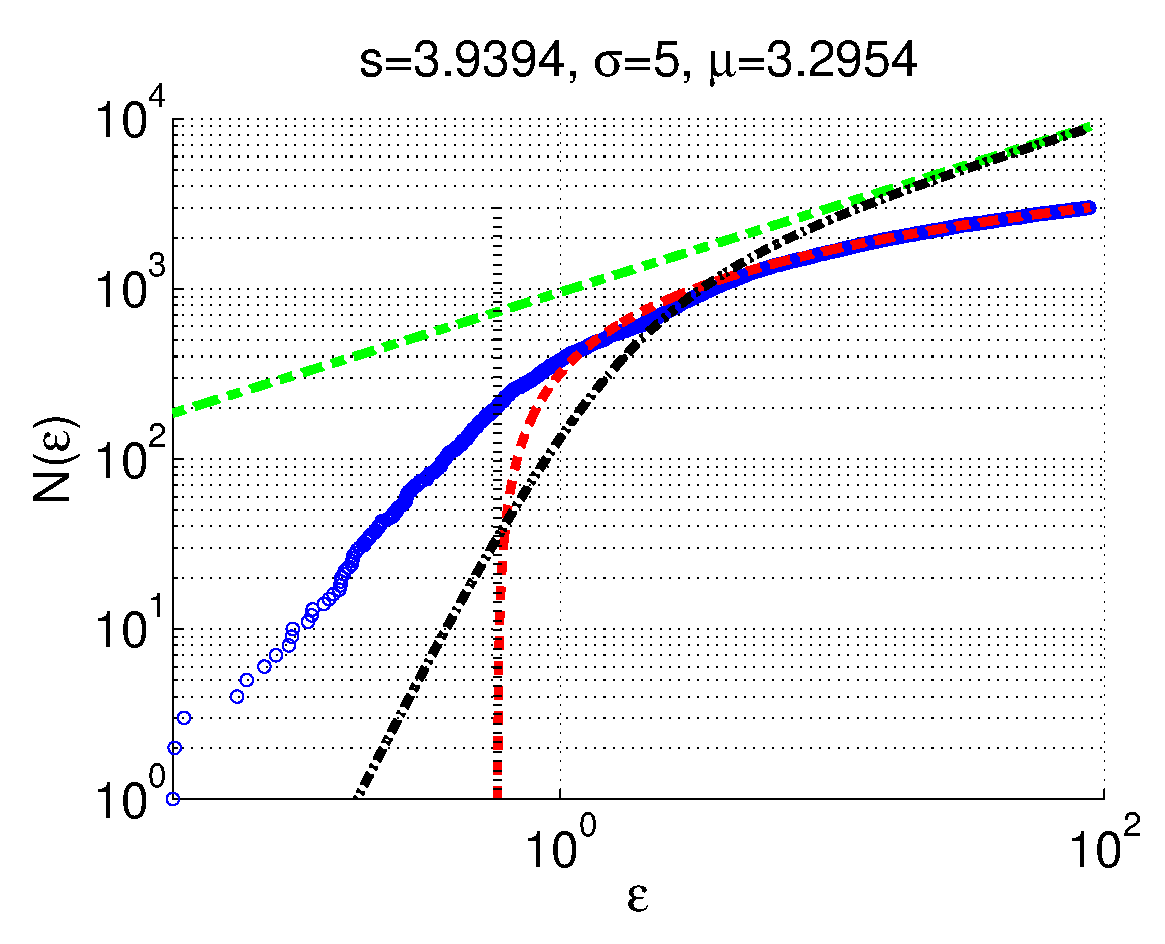
\includegraphics[height=4.5cm]{/Figs/NumStates_40}
%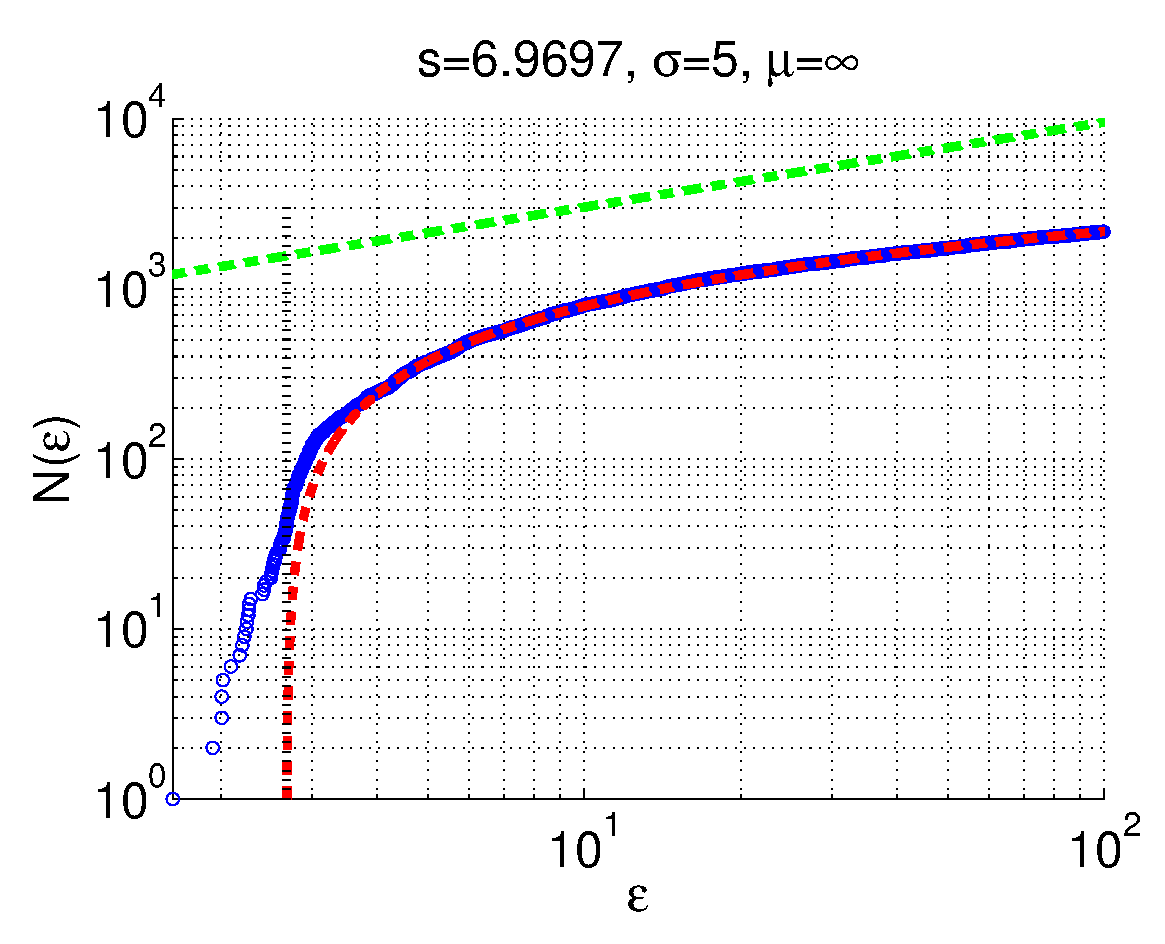
\includegraphics[height=4.5cm]{/Figs/NumStates_70}
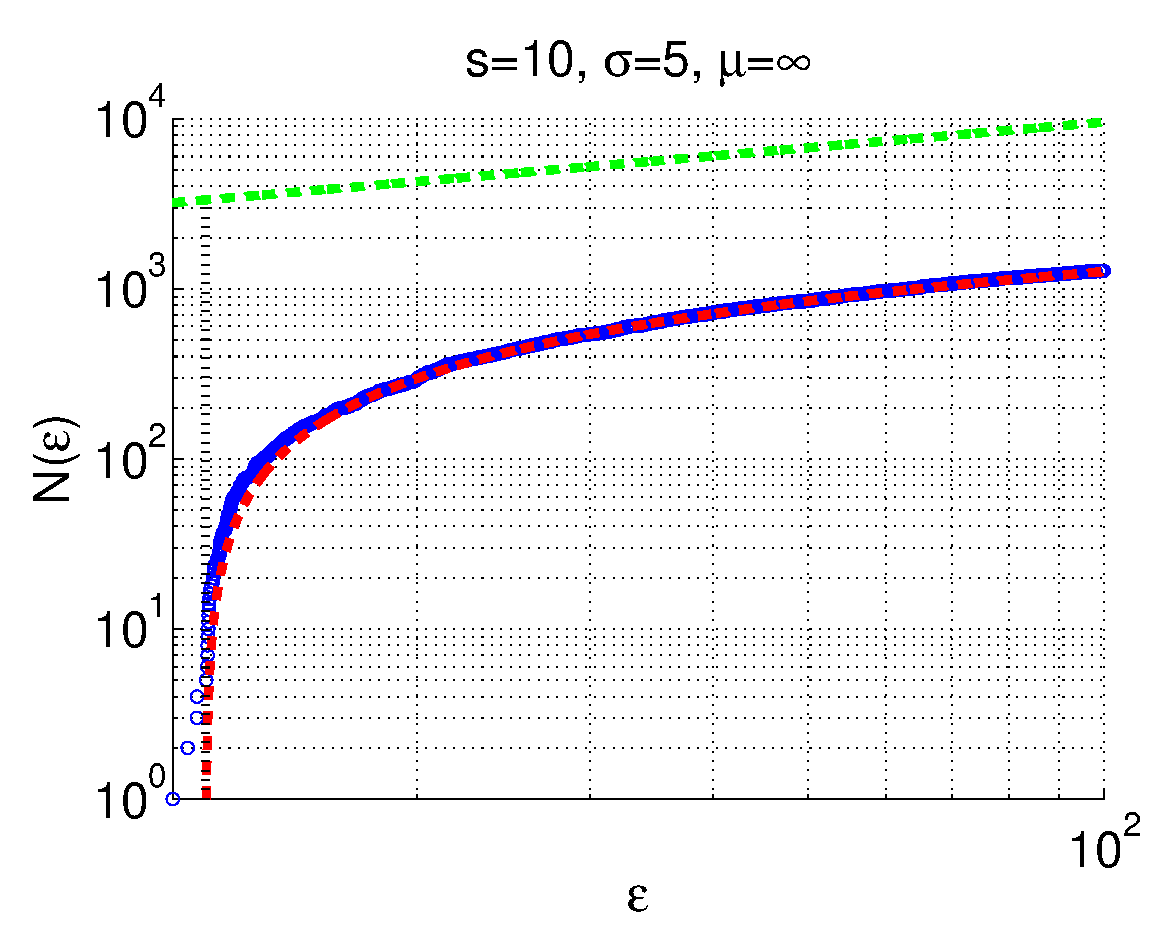
\includegraphics[height=4.5cm]{/Figs/NumStates_100}

\caption{Integrated density of states.
The blue points are calculated from numerical diagnoalization. 
The red line dashed curve corresponds to the log-box result (large $s$), \Eq{e92}.
The black dashed-dot line is \Eq{e93} and the green line is just a free particle \Eq{e94}.
The vertical dotted line is $\varepsilon=\exp[(s-\sigma)/2]$.
}
\label{NumStates}
\end{figure}





%%%%%%%%%%%%%%%%%%%%%%%%%%%%%%%%%%%%%%%%%%%%%%%%%%%%%%%%%%%%%%%
%\hide{\clearpage
%\sect{The ABAB model}
%
%Consider the simplest model with "disorder". A lattice of period $N=2$, with transition rates 
%$\ln(\ora{A}/\ola{A}) = s+\sigma$ and $\ln(\ora{B}/\ola{B}) = s-\sigma$.
%The Derrida criterion is $s_c = \ln(\cosh \sigma)$
%
%\begin{figure}[h]
%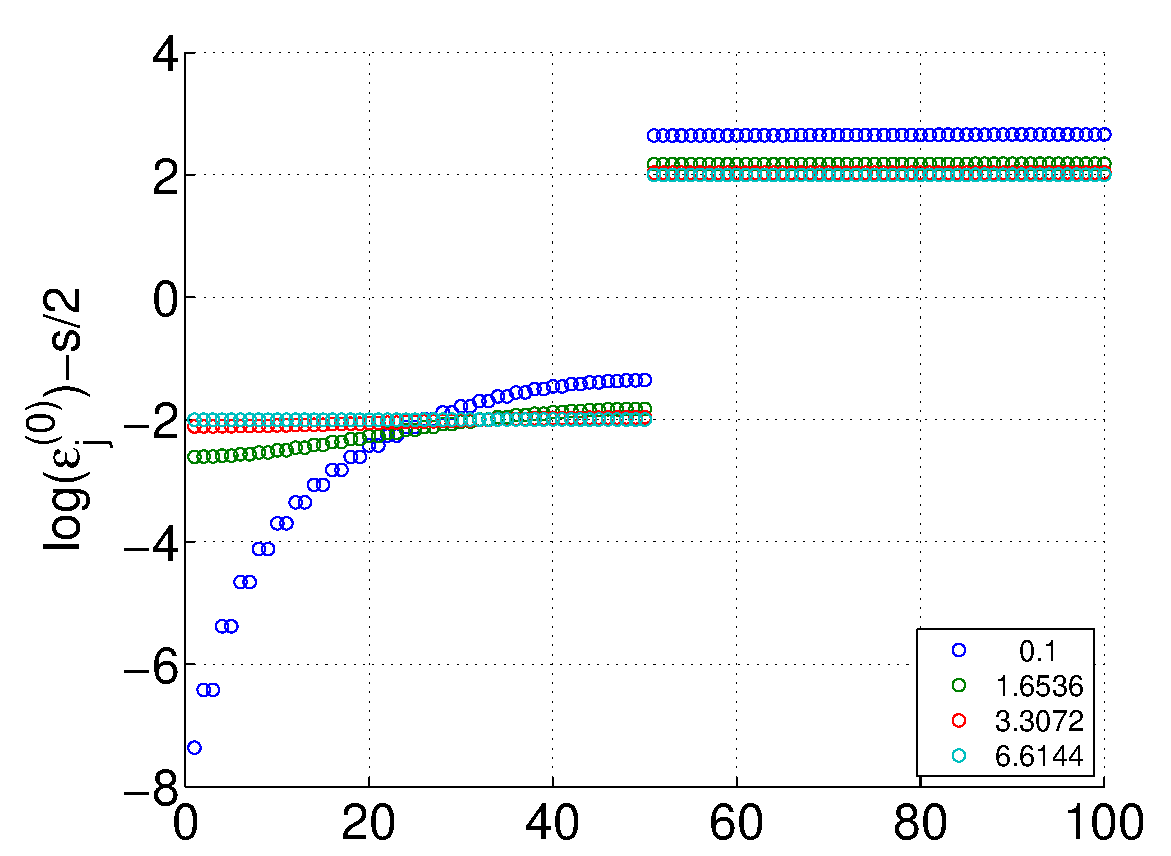
\includegraphics[height=5cm]{/Figs/epsilon_j_N_2.eps}
%\includegraphics[height=5cm]{/Figs/kappa_N_2.eps}
%\caption{The eigenvalues $\varepsilon_j^{(0)}$ (left) for $\sigma=4$ and varying $s$ (see legend)
%and the inverse localisation length $\kappa$ (right)
%The red line is for $s=s_c$}
%\label{fig10}
%\end{figure}
%
%\clearpage
%}
%%%%%%%%%%%%%%%%%%%%

\sect{The spectrum of a disordered ring}

We plot the equation 
%
\be{69}
\sum_{j=1}^N \log\left(|\lambda - \varepsilon_j(s)|\right)  \ = \ 
\log \left[2\left(\cosh\left(\frac{sN}{2}\right) -1\right)\right]
\ee
%
The interesting behavior is at the bottom of the spectrum. 
Large values of $\lambda$ simply correspond to a clean ring. 
The condition for complexity is that  $\kappa<\log \left[2\left(\cosh\left(\frac{sN}{2}\right) -1\right)\right]$.
Focusing on the lower region of the spectrum we see that 
%
\begin{enumerate}
\item For $s<s_{1/2}$,  $\kappa$ is convex with a minimum at the origin (the spectrum is real). 
\item In the vicinity of the sliding transition $s\approx s_1$, $\kappa$ is concave but very shallow (the spectrum is complex). 
\item For large values of $s>s_1$, $\kappa$ is concave with a minimum far from the origin (the spectrum is complex). 
\end{enumerate}
%
It is possible to obtain analytical expressions for the envelope function 
in the limits of weak and strong disorder, as will be shown in the following sections. 
However, the observations regarding the shape of $\kappa$ 
and the ensuing consequences for the complexity of the spectrum  
are easily explained by the electrostatic analogy. 
%
For $s<s_{1}$ there is an accumulation of charge at the origin (the "spectral condensate", see \Fig{DOS}), 
this pulls the minimum of the potential to the origin as well, leading to the convex structure of the envelope function (actually, the minimum at the origin appears for $s<s_{1/2}$). 
As a result, all eigenvalues are real. 
Once $s>s_{1/2}$ the charges spread out along the axis (see \Fig{DOS}) and the minimum moves away from the origin, 
leading to a concave envelope function and complex eigenvalues. 


%%
%\begin{figure}[h]
%\includegraphics[height=5cm]{/Figs/gap_s_N.eps}
%\includegraphics[height=5cm]{/Figs/envelope_10.eps}
%\includegraphics[height=5cm]{/Figs/envelope_21.eps}
%\includegraphics[height=5cm]{/Figs/envelope_27.eps}
%\includegraphics[height=5cm]{/Figs/envelope_40.eps}
%\includegraphics[height=5cm]{/Figs/envelope_50.eps}
%\caption{$\kappa(\lambda)$ (green) along with oscillating function (blue) for various values of $s$ corresponding to the points indicated 
%on the plot of the gap. The dashed red line is $s/2$. }
%\end{figure}

%
%\begin{figure}[h]
%\ \ \ \ \ \ \includegraphics[width=7cm]{/Figs/fieldlines_a.eps}
%
%\includegraphics[width=7.5cm]{/Figs/kappa_a.eps}
%\caption{ Top: Field lines, red line is the equipotential line $s/2$. Bottom: $\kappa$. Here $N=100$ sites.
%There is some correspondence between the "bubble" structure of the equipotential lines and the structure of 
%$\kappa$ }
%\end{figure}



%%%%%%%%%%%%%%%%%%%%%%%%%%%%%%%%
\subsect{Large $s$ (weak disorder)}

When is $s$ is large compared with $s_{\infty}\sigma$, 
the density of states of  the associated Hermitian matrix is $\rho(x)=N/(\sigma x)$.
The integral can be calculated analytically.
Specifically, the envelope $\kappa$ is just the potential along the real axis. 
The endpoints of the charged bar are 
%
\beq
a \ =\ e^{(s-\sigma)/2}\ , \ \ b \ =\ e^{(s+\sigma)/2}
\eeq
%
we obtain
%
\be{91}
\kappa(x) &=& \varphi(x,0) = 
\frac{1}{\sigma}\int_{e^{(s-\sigma)/2}}^{e^{(s+\sigma)/2}}
 \frac{\ln(x-x')}{x'}dx' =\\
%&=& \text{Re}\left\{
%\sigma \log(x) + \text{Li}_2 \left[ e^{(s-\sigma)/2}/x \right] -  \text{Li}_2 \left[ e^{(s+\sigma)/2}/x \right]\right\} \\
&=&
 \ln(|b - x|) \ln\left(\frac{b}{x}\right) + \ln(|x-a|) \ln \left(\frac{x}{a}\right) +
   \text{Li}_2\left( 1 -\frac{b}{x}\right) + \text{Li}_2\left( 1-\frac{a}{x}\right) 
\ee
%
In \Fig{figWeak} we show the envelope function $\kappa(x)$ along the real axis
and the corresponding electrostatic potential and field lines.
The potential has a global minimum far from the origin, and a large region of the spectrum is complex. 
%
The integrated density of states is 
%
\be{92}
 \mathcal{N}(\varepsilon)=\frac{N}{\sigma} \left [\ln(\varepsilon) -\frac{s-\sigma}{2}\right]
\ee
%
\begin{figure}[h!]
 \includegraphics[width=7cm]{/Figs/kappa_large_S}

\ \ \ \includegraphics[width=8.5cm]{/Figs/electrostatics_large_S}

\ \ \ \includegraphics[width=5cm]{/Figs/electrostatics_large_S_zoom}

\caption{ Top: $\kappa$. The green points are the result of numerical diagonalization, the dashed blue line is 
the analytical result assuming $\rho=(\sigma x)^{-1}$. The stars 
indicate the position of the "charges", which are the eigenvalues of the associated Hermitian matrix, $\varepsilon_j$.
Bottom: Field lines of the corresponding electrostatic problem. The red line is the equipotential line $s/2$ Here $N=100$ sites, $\sigma=2$ and $s=5$.
}
\label{figWeak}
\end{figure}
%
%
Near the origin, the contour $\varphi(x,y) = s/2$ can be approximated 
by expanding the integrand of \Eq{e65} in $x$ and $y$ and the integrating with respect to $x'$. 
The equation  $\varphi(x,y) = \varphi(0,0)$ then is solved by the parabola
%
\beq
x =  Cy^2
\eeq
%
where the curvature is 
%
\beq
C \equiv \frac{1}{2}e^{-s/2}\cosh\left(\frac{\sigma}{2}\right) y^2 
\eeq
%
%
and the gap $\Delta_{\lambda}$ is given by the expression
%
\beq
\int_{0}^{\sqrt{\Delta_{\lambda}/C}} \left|\vec{E}(x,y)\right| dy \ = \ 2\pi
\eeq
%
This is equivalent, through Cauchy Riemann, to the requirement $\psi(\Delta_{\lambda},0)=2\pi$.
%
The integrand is approximated by $|\vec{E}(x,y)| \approx |\vec{E}(0,0)|$ by which we obtain
an estimate for the gap
%
\be{95}
\Delta_{\lambda} \approx \frac{4\pi^2 C}{ \left|\vec{E}(0,0) \right|^2} =\frac{ 2\pi^2 }{N^2} \exp\left(s/2-s_{1/2}\right)\cosh\left(\frac{\sigma}{2}\right)
\ee
%
where the field magnitude at the origin is 
%
\beq
\left|\vec{E}(0,0) \right| = \left|E_x(0,0) \right| = \frac{N}{\sigma} \int_a^b \frac{dx}{x^2} = 
%&=& \frac{1}{\sigma}\left(e^{-(s-\sigma)/2} - e^{-(s+\sigma)/2}\right) =
\frac{2N}{\sigma} \sinh \left( \frac{\sigma}{2} \right) e^{-s/2} \ = \ Ne^{(s_{1/2}-s)/2}
\eeq
%
Note that the coulomb integral for the electric field of a wire in two dimensions is
%
\beq
E_x = \int_a^b \frac{x-x'}{(x-x')^2 + y^2}\rho(x')dx' \\
E_y = \int_a^b \frac{y}{(x-x')^2 + y^2}\rho(x')dx' \\
\eeq
%
and at the origin
%
\beq
E_x(0,0) \ =\  \int_a^b \frac{\rho(x)}{x}dx \\
\eeq
%

\subsect{The complex gap - Generalization}

We expand the potential in a series around the origin
%
\beq
\varphi(x,y) &=& \frac{1}{2}\int_a^b \ln \left((x-X)^2 + y^2\right) \rho(X) dX \\
&\approx & \int \left(\ln(X) -\frac{x}{X} + \frac{1}{2} \frac{y^2}{X^2} + \frac{xy^2}{X^3}\right)\rho(X) dX = \\
&=& C_0 - C_1 x +\frac{1}{2}C_2y^2 + C_3 xy^2
\eeq
%
where the coefficients $C_n$ are defined 
%
\beq
C_n = \int_a^b \frac{1}{x^n}\rho(x)dx
\eeq
%
Notice that 
%
\beq
C_0 = \varphi(0,0), \ \ C_1 = E(0,0)
\eeq
%
%
Since we are interested in the contour $\varphi(x,y) = \varphi(0,0)$, we obtain
%
\beq
x = \frac{C_2}{2C_1} y^2 
\eeq
%
From \Eq{e95} we obtain the expression
%
\be{96}
\Delta_{\lambda} \ = \ 2\pi^2 \frac{C_2}{|C_1|^3} \sim \frac{1}{N^2}
\ee
%
\subsect{Small $s$ (strong disorder)}

For small $s$, the envelope function increases from zero and is convex. 
This is due to the fact that there is a "spectral condensate" at $\varepsilon=0$. 
We verify this by manually removing the condensate from the spectrum and recalculating 
the envelope function.
%
In fact, the exact formulas for the integrated density of states $N(E)$ and $\kappa(E)$ in the continuum limit are available due to \cite{odh3}.
We define 
%
\beq
z = 2304\frac{D_0^3}{\sigma^4} \varepsilon 
\eeq
%
So the integrated density of states is 
%
\be{93}
\mathcal{N}(z)   \ &=& \ \frac{\sigma^2 N}{24\pi^2}\frac{1}{ M_{\mu}^2 (\sqrt{z})}
\ee
%
Note that in the limit $\varepsilon\to \infty$ the free particle result is recovered
%
\be{94}
\mathcal{N}(\varepsilon) = \frac{N}{\pi} \sqrt{\varepsilon}
\ee
%
The inverse localization length in \cite{odh3} is
%
\beq
\kappa(z) \ = \ -\sqrt{z} \frac{M'_{\mu}(\sqrt{z})}{M_{\mu}(\sqrt{z})} \frac{\sigma^2}{48D_0^2}, \ \ z \geq 0
\eeq
%
where
\beq
M_{\mu}(z) &=& \sqrt{J(z)^2_{\mu} + Y(z)^2_{\mu}}
\eeq
%

and $J_{\mu}$ and $Y_{\mu}$ are Bessel functions of the first and second kind.
%
In the limit $\varepsilon \to 0$ we have for $\mu>0$
%
\beq
\mathcal{N}(\varepsilon) &\propto & N\sigma^{2-4\mu}\varepsilon^{\mu}\\
\rho(\varepsilon) &=& \frac{d\mathcal{N}}{d\varepsilon} \sim  \mu \varepsilon^{\mu - 1} \\
\kappa(\varepsilon) &=& 
\left\{
\begin{array}{cc}
\mu \nearrow 1/2, \ &  \mu<1/2 \\
\mu \searrow 1/2, \ &  \mu>1/2 
\end{array}\right.
\eeq
%
The spectral condensate occurs for $\mu<1$, however this condition does not ensure that 
$\kappa$ has a maximum (global minimum at the origin). 
The requirement for  $\kappa$ to have a maximum is the more stringent $\mu<1/2$. 
At $\mu=1/2$, $\kappa$ is flat.
%
Since $\kappa(E\to \infty) = 1/2$ for all $\mu$, for $\mu>1/2$ 
the spectrum becomes entirely complex, 
whereas in the discrete model only a finite fraction of the eigenvalues can be complex (see \Fig{figCplxSat}).
%
\begin{figure}[h]
 \includegraphics[width=5cm]{/Figs/P_E_small_S}
 \includegraphics[width=5cm]{/Figs/kappa_small_S}
  \includegraphics[width=5cm]{/Figs/kappa_small_S_zoom}
\caption{ 
On the left we show the density of states for $s<s_c$. There is a spectral condensate at the origin (red bar).
The envelope function $\kappa$ is plotted on the right (green line) and it is convex near the origin . If the condensate is removed (magenta) a concave envelope function is obtained. 
In the bottom figure, we zoom in on the lower band and plot the exact result (dashed black curve).
}
\end{figure}
%

For $s<s_{1/2}$ the density of state of the hermitian problem and the non hermitian problem are approximately equal (\rmrk{I assume this by observing numerically that  $\Delta_{\lambda}$ vs. 
$\Delta_{\varepsilon}$ for different values of $N$ has a linear correlation}). So we can deduce the value of the gap in this region 
simply by setting $\mathcal{N}(\Delta_{\lambda}) = 1$ in \Eq{e93}
%
\beq
\Delta_{\lambda} \approx \Delta_{\varepsilon}  = \left(\frac{24\pi^2}{N}\right)^{\mu}\sigma^{4-2/\mu}
\eeq
%
%%%%%%%%%%%%%%%%%%%%%%%%%
%%%%%%%%%%%%%%%%%%%%%%%%%%%%%%%%%%%%%%%%

\subsect{The Gap}

There are two factors that determine the gap. 
The distribution of charges and the height of the equipotential contour, namely the value of $s/2$. 
The distribution of charges determines where the field lines depart from the $x$-axis and the value $s/2$ determines the "radius" of the contour.
%
For $s_{1/2}<s<s_1$ the departure point and the radius grow together. 
For $s_1<s<s_2$, the radius grows but the departure point moves toward the origin.
For $s\gg s_2$, they both grow together again.
%\begin{figure}[h!]
%%10,20,27,40,70
%\includegraphics[height=5cm]{/Figs/gap_3000_guide.eps}
%\includegraphics[height=5cm]{/Figs/electrostatics_10}
%\includegraphics[height=5cm]{/Figs/electrostatics_20}
%\includegraphics[height=5cm]{/Figs/electrostatics_22}
%\includegraphics[height=5cm]{/Figs/electrostatics_27}
%\includegraphics[height=5cm]{/Figs/electrostatics_32}
%\includegraphics[height=5cm]{/Figs/electrostatics_40}
%\includegraphics[height=5cm]{/Figs/electrostatics_70}
%\caption{Depicting the gap in the electrostatic analogy. 
%The electrostatic potential (thin blue lines) and field lines (thick lines) are plotted 
%for various values of $s$, indicated by markers on the top left panel. The green dots 
%represent the position of the charges and the red contour is $\phi=s/2$. 
%}
%\label{electrostatics_gap}
%\end{figure}

\clearpage
\sect{Complexity saturation}

The secuar equation for the eigenvalues is given by \Eq{e69}
%
\beq
\sum_{j=1}^N\log \left[ \lambda - \varepsilon_j(s)\right]=
 \log \left[2\left(\cosh\left(\frac{sN}{2}\right) -1\right)\right] 
\eeq
%
where the left hand side is the envelope function $\kappa(\lambda)$. 
The eigenvalues for which $\kappa(\lambda)>\log\left[2\left(\cosh\left(\frac{sN}{2}\right) -1\right)\right]$
are real.
%
In the nonconservative case, one can raise the horizontal line (right hand side of \Eq{e69}) by increasing $s$,
thus making the entire spectrum complex. 
For a conservative matrix, however, $\kappa$ is also a function of $s$, so increasing $s$ raises $\kappa$ 
more or less at the same rate, leaving the number of intersections unchanged, see \Fig{fig7}.
%
This claim can be seen from \Eq{e69}.
Due to the conservative property, the $\sigma$ disorder is in fact diagonal disorder. Therefore, for large enough $s$, the eigenvalues of the associated hermitian martix, $\varepsilon_j$ 
grow proportionaly to $\exp (s)$. 
Increasing $s \to s+\Delta s$, we have
%
\beq
\sum_{j=1}^N \log \left(\lambda - \varepsilon_j e^{\Delta s}\right) &=&
 \log \left[2\left(\cosh\left(\frac{(s+\Delta s)N}{2}\right) -1\right)\right] \\
\sum_{j=1}^N \log\left(\lambda e^{-\Delta s} - \varepsilon_j 
 \right) 
 + N\Delta s &=&
 \log \left[2\left(\cosh\left(\frac{sN}{2}\right) -1\right)\right] +N\Delta s\\ 
\eeq
%
But $\lambda$ is just a dummy variable, so we can redefine $\lambda := \lambda e^{-\Delta s}$ and the equation is unchanged. Thus increasing $s$ does not change the number of complex solutions.




%%%%%%%%%%%%%%%%%%%%%%%%%%%%%%%%%%%%%%%%%%%%%%%%%%%%%%%%%%%%%%%%
\begin{figure}[h]
\includegraphics[height=4cm]{/Figs/kappa_4a.eps}
\includegraphics[height=4cm]{/Figs/kappa_4.eps}
\caption{
The inverse localization length $\kappa$ vs. $\varepsilon$ for ${N=20, \ \sigma=4, \ \Delta=0}$, $s=0.1$ (red), $s=3$ (green) and $s=20$ (blue). The dashed lines are the right hand side of \Eq{e69}.
In the right panel, the horizontal axis is $\varepsilon e^{-s/2}$ and the vertical axis is $ \kappa-s/2$.
}
\label{fig7}
\end{figure}
%
%%%%%%%%%%%%%%%%%%%%%%%%%%%%%%%%%%%%%%%%%%%%%%%%%%%%%%%%%%%%%%%%%

\subsect{Estimating the fraction of complex eigenvalues}

We estimate the the saturation value of the fraction of complex eigenvalues.
This means we are interested in the region $s > s_1$.
The eigenvalues have a $\rho\sim1/x$ distribution and the inverse localization length, $\kappa(x)$ is given by \Eq{e91}.
Define $x_0$ such that the eigenvalues in the range $\exp[(s-\sigma)/2] < x < x_c$ are complex, $x_0$ is determined by the equation
%
\beq
\kappa(x_c) = \frac{s}{2}
\eeq
%
The fraction of complex eigenvalues  is just 
%
\be{101}
n =\frac{ \int_a^{x_c}  \frac{1}{ x} dx}{ \int_a^{b}  \frac{1}{ x} dx} = 
\frac{1}{\sigma}\ln\left( \frac{x_c}{a} \right) = 
\frac{\ln x_c - \frac{s-\sigma}{2}}{\sigma}
\ee
%

%

\clearpage
\subsect{Effect of glassiness on complexity saturation}

The effect of glassiness, or offdiagonal disorder ($\Delta$) is to further supress the complexity, however now the plateau becomes fuzzy, as seen in \Fig{fig8}. This happens because the off diagonal disorder spreads out the eigenvalues as in \Fig{fig9}.
For large $s$, the eigenvalues are approximated by the diagonal elements
%
\beq
\varepsilon_j \approx \exp \left[-B_j + \mathcal{E}_j \right] \sim \exp\left[-B_j +\frac{s}{2}\right]
\eeq
%
%%%%%%%%%%%%%%%%%%%%%%%%%%%%%%%%%%%%%%%%%%%%%%%%%%%%%%%%%%%%%%%
\begin{figure}[h]
\includegraphics[height=4cm]{/Figs/num_cplx_Delta.eps}
\includegraphics[height=4cm]{/Figs/num_cplx_Delta_sigma.eps}
\caption{The number of complex eigenvalues for $\Delta=1$ (red) and $\Delta=5$ (green) for $\sigma=0$ (left panel) and $\sigma = 3$ (right panel).
}
\label{fig8}
\end{figure}
%
%%%%%%%%%%%%%%%%%%%%%%%%%%%%%%%%%%%%%%%%%%%%%%%%%%%%%%%%%%%%%%%
\begin{figure}[h]
\includegraphics[height=4cm]{/Figs/epsilon_j.eps}
\includegraphics[height=4cm]{/Figs/kappa_Delta.eps}
\caption{The eigenvalues $\varepsilon_j^{(0)}$ for $\sigma=3$ and varying $\Delta$ (see legend). As $\Delta$ increases, the eigenvalues spread out (left panel), the dashed  black horizontal line is $s/2$. As a result, 
there are more real eigenvalues(right panel).
}
\label{fig9}
\end{figure}

\clearpage

\rmrk{\bf Excluded material}

\rmrk{The following figures show how the spectrum evolves with $s$, however this is unnecessary due to the electrostatic pictures. 
However, the figures are illustrative.}
%%%%%%%%%%%%%%%%%%%%%%%%%%%%%%%%%%%%%%%%%%%%%%%%%%%%%%%%%%%%%%%%
\begin{figure}[h]
\includegraphics[height=5cm]{/Figs/kappa_1_a.eps}
\includegraphics[height=5cm]{/Figs/epsilon_s_1_a.eps}
\includegraphics[height=5cm]{/Figs/kappa_2_a.eps}
\includegraphics[height=5cm]{/Figs/epsilon_s_2_a.eps}
\caption{
Top row: The inverse localization length $\kappa$ vs. $\varepsilon$ (left panel) for ${N=20, \ \sigma=1}$, $s=0.1$ (red) and $s=3$ (green). The dashed lines are the right hand side of \Eq{e69}.
For small $s$ all eigenvalues are real, for large $s$, only two are real.
The right panel shows the trajectories of the eigenvalues  in the complex plane as $s$ is increased. 
The green and red dots correspond to the lines of the left panel.
Notice that $\varepsilon=0$ is always a solution.
Bottom row: same as top row, but here $\sigma=4$ and $s=0.1$ (red) and $s=5$ (green).
}
\label{fig6}
\end{figure}
%%%%%%%%%%%%%%%%%%%%%%%%%%%%%%%%%%%%%%%%%%%%%%%

%\section{Appendix - Diffusion equation with drift and varying diffusion coefficient}
%Consider the diffusion equation on a one dimensional ring $x\in [0,L]$
%%
%\be{1}
%\frac{\partial \psi}{\partial t} = \frac{\partial }{\partial x} \left[ D(x) \frac{\partial \psi}{\partial x}\right] - v\frac{\partial \psi}{\partial x}
%\ee
%%
%with diffusion coefficient 
%%
%\beq
%D(x) = \left\{ \begin{array}{cc}
%D_0, & |x|<a/2 \\
%D, & |x|>a/2 
%\end{array}
%\right.
%\eeq
%% 
%We will refer to this configuration as a "diffusion barrier".
%
%We ask the question - under what conditions is the reality of the spectrum broken. 
%Specifically we are interested in the limit $a\to 0$.
%%
%The solution to the diffusion equation in each region is  simply  $\psi \sim e^{-\lambda t + ikx}$, inserting this in \Eq{e1}, we obtain the dispersion relation 
%%
%\beq
%\lambda &=& Dk^2 + ivk\\
%k_{\pm} &=& \frac{-iv \pm \sqrt{4\lambda D -v^2}}{2D} = \frac{-is}{2} \pm \sqrt{\frac{\lambda}{D}-\frac{s^2}{4}}
%\eeq
%%
%So the solution to \Eq{e1} has the form 
%\be{2}
%\psi(x) = Ae^{ik_{+} x}+ Be^{ik_{-} x} = \eexp{\frac{v}{2D}x} \left(Ae^{i\frac{\sqrt{4\lambda D -v^2}}{2D}x}+Be^{-i\frac{\sqrt{4\lambda D -v^2}}{2D}x}\right)
%\ee

%%%%%%%%%%%%%%%%%%%%%%%%%%%%%%%%%%%%%%%%%%%%%%%%%%%%
%%%%%%%%%%%%%%%%%%%%%%%%%%%%%%%%%%%%%%%%%%%%%%%%%%%%
%
%\subsection{Simple cases}
%
%Let us first consider the simplest cases of a ring with and without drift and $D(x)=D$,
%We then compare to a chain (Neumann or Dirichlet boundary conditions)
%\begin{enumerate}
%\item
%$D(x)=D, \ v=0$ and periodic boundary conditions $\psi(0)=\psi(L), \ \psi'(0)=\psi'(L)$, we obtain the eigenvalues $-\lambda$
%%
%\be{3}
%\lambda  = Dk^2 =D\frac{4\pi^2 n^2}{L^2}
%\ee
%%
%So of course the spectrum is real. 
%%
%
%\item
% $D(x)=D, \ v/D=s \neq 0$ and periodic boundary conditions $\psi(0)=\psi(L), \ \psi'(0)=\psi'(L)$, we obtain the eigenvalues $-\lambda$
%%
%\be{4}
%\lambda &=&  D\frac{4\pi^2 n^2}{L^2}-i\omega n \\ 
%\omega &=& \frac{2\pi v}{L}
%\ee
%%
%The spectrum is complex except for $\lambda = 0$.
%\item  $D(x)=D, \ v/D=s \neq 0$  Neumann boundary conditions yield
%%
%\be{5}
%\lambda &=& D\frac{\pi^2 n^2}{L^2} + \frac{v^2}{4D}\\ 
%\lambda &=& 0
%\ee
%%
%Again, the spectrum is entirely real. 
%\end{enumerate}

\clearpage
%%%%%%%%%%%%%%%%%%%%%%%%%%%%%%%%%%%%%%%%%%%%%%%%%%%%
\sect{Appendix: Secular equation for the clean ring}

The wave function can be written
%
\beq
\psi(x) = Ae^{ik_{+} x}+ Be^{ik_{-} x} = \eexp{\frac{v}{2D}x} \left(Ae^{i\frac{\sqrt{4\lambda D -v^2}}{2D}x}+Be^{-i\frac{\sqrt{4\lambda D -v^2}}{2D}x}\right)
\eeq
%
Periodic boundary conditions on $\psi(x)$ and $\partial \psi(x)$
%
\beq
A+B \ &=& \ A e^{ik_+L}  + B e^{ik_-L}  \\
ik_{+} A + ik_{-} B \ &=& \ ik_{+} A e^{ik_+L}  + ik_{-} B e^{ik_-L} 
\eeq
%
Non trivial solutions are given by the equation 
%
\beq
\left( k_{-}-k_{+}\right) \left(1- e^{ik_-L} - e^{ik_+L}  - e^{i(k_- + k_+) L}\right) =0
\eeq
%
from which two equations are obtained
%
\beq
 \cos \left ( \sqrt{\frac{4\lambda}{D} - \frac{v^2}{4D^2}}L \right) &=& \cosh\left(\frac{v}{2D}L\right)
 \eeq
 %
% and
% %
% \beq
% \lambda & = & \frac{v^2}{4D}
%\eeq


%%%%%%%%%%%%%%%%%%%%%%%%%%%%%%%%%%%%%%%%%%%%%%%%%%%%
\sect{Appendix: Diffusion equation matching conditions }

We consider two types of boundaries. The first case is when there is a jump in the diffusion coefficient. 
Specifically we are interested in the limit where the jump region $a$ is small and the jump is large. 
We call this a diffusive scatterer. 
The second case is a jump in the velocity. 

\subsect{Diffusive scatterer}


The diffusion barrier is defined as 
%
\beq
D(x) = \left\{ \begin{array}{cc}
D_0, & |x|<a/2 \\
D, & |x|>a/2 
\end{array}
\right.
\eeq
%
Requiring that the diffusion equation \Eq{e11} be continuous dictates that 
the distribution function $\psi(x)$ 
and the current $D(x)\partial_x \psi(x)-v\psi(x)$ 
be continuous.
This is in contrast to the Schroedenger equation, 
where the continuity requirement is on the derivative $\partial_x\psi(x)$ and not on the current. 
Let us denote the wave function inside the barrier $|x|<a/2$ as $\psi_0$. Outside, it is $\psi$.
%
\beq
\psi_0 &=& A e^{ik_0x} + Be^{-ik_0x} \\
\partial \psi_0 &=& ik_0\left(A e^{ik_0x} - Be^{-ik_0x}\right) \\
\eeq
%
where $k_0 = \sqrt{\lambda/D_0}$.
Since we will later take the limit $a\to 0$, we assume that the drift term doesn't play a role within the diffusion barrier. 

Inside the barrier, the probability distribution is freely propagating. The values of $\psi_0$ and $\partial\psi_0$ at each of the boundaries $x=\pm a/2$ can be shown to be  related by the linear equation
%
\beq
\left.\left( \begin{array}{c}
\psi_0 \\
\partial \psi_0
\end{array}
\right)\right|_{-a/2} = 
\left( \begin{array}{cc}
\cos(k_0a) & \frac{1}{k_0} \sin{k_0a} \\
-k_0 \sin{k_0a} & \cos(k_0a)
\end{array}
\right)
\left.\left( \begin{array}{c}
\psi_0 \\
\partial \psi_0
\end{array}
\right)\right|_{a/2} 
\eeq
%

And requiring continuity of the distribution and the current, we can stitch the interior solution $\psi_0$ to the exterior solution $\psi$
%
\beq
\left.\left( \begin{array}{c}
\psi\\
\partial \psi
\end{array}
\right)\right|_{-a/2}  = 
%\left( \begin{array}{cc}
%1 & 0 \\
%0 & \frac{D_0}{D}
%\end{array}
%\right)
%\left( \begin{array}{cc}
%\cos(k_0a) & \frac{1}{k_0} \sin{k_0a} \\
%k_0 \sin{k_0a} & \cos(k_0a)
%\end{array}
%\right)
%\left( \begin{array}{cc}
%1 & 0 \\
%0 & \frac{D}{D_0}
%\end{array}
%\right)
%\left.\left( \begin{array}{c}
%\psi \\
%\partial \psi
%\end{array}
%\right)\right|_{a/2} = \\
\left( \begin{array}{cc}
\cos(k_0a) & \frac{D}{D_0 k_0} \sin{k_0a} \\
-\frac{D_0 k_0}{D} \sin{k_0a} & \cos(k_0a)
\end{array}
\right)
\left.\left( \begin{array}{c}
\psi \\
\partial \psi
\end{array}
\right)\right|_{a/2}
\eeq
%
Taking, carefully, the limit $a\to 0$, 
%
\beq
\left.\left( \begin{array}{c}
\psi\\
\partial \psi
\end{array}
\right)\right|_{-a/2}  \approx
\left( \begin{array}{cc}
1 & D\frac{a}{D_0 }  \\
0 & 1
\end{array}
\right)
\left.\left( \begin{array}{c}
\psi \\
\partial \psi
\end{array}
\right)\right|_{a/2}
\eeq
%
rewriting these two equations explicitly, we obtain the diffusion barrier matching conditions
%
\be{61}
\psi(a/2)-\psi(-a/2) &=& -\frac{a}{D_0}D \partial \psi(a/2)\\
\partial \psi(a/2) &=& \partial \psi(-a/2) 
\ee
%
To check, notice that if $D_0 \to 0$ faster than $a\to 0$, Neumann boundary conditions are recovered.\\
If $D_0=D$, periodic boundary conditions are recovered. 
The matching conditions of \Eq{e61} can be written in matrix form with the matching matrix $M$
%
\beq
M = 
\left( \begin{array}{cc}
1 & D\frac{a}{D_0 }  \\
0 & 1
\end{array}
\right)
\eeq

Let us define 
%
\beq
\alpha = \frac{a}{D_0}, \ \ g \ = \ \frac{a}{L} \cdot \frac{D}{D_0}
\eeq
%
as the strength of the diffusion barrier, 
in analogy with a delta function potential  $u\delta(x)$ in the Schroedenger equation.


\subsect{Jump in the velocity}

The velocity $v(x)$ in the diffusion equation is 
%
\beq
v(x) = \left\{ \begin{array}{cc}
v_1, & 0< x<L/2 \\
v_2, & L/2<x<L
\end{array}
\right.
\eeq
%
with
% 
\beq
v_1 &=& s_1 D = D(s+\sigma)\\
v_2 &=& s_2 D = D(s-\sigma)
\eeq
%
Continuity of the diffusion equation across the boundaries requires that 
the distribution $\psi$ and the current $D\partial \psi -v \psi$ be contiuous across the boundaries
%
\beq
\left( \begin{array}{c}
\psi_1 \\
\partial \psi_1
\end{array}
\right) \ = \
%
M(v_1-v_2)
%
\left( \begin{array}{c}
\psi_2 \\
\partial \psi_2
\end{array}
\right)
\eeq
%
where
%
\beq
M(u) \equiv
\left( \begin{array}{cc}
1 &0  \\
\frac{u}{D} & 1
\end{array}
\right)
\eeq
%

%%%%%%%%%%%%%%%%%%%%%%%%%%%%%%%%%%%%%%%%%%%%%%%%%%%%
\sect{Appendix: Secular equation for ring + g}

The transfer matrix across a segment of length $L/2$ is 
%
\beq
T(s,k;L/2)\equiv
\frac{e^{s L/4}}{k}
\left(
\begin{array}{cc}
-\frac{s}{2}\sin\left(\frac{k L}{2}\right) + k\cos \left(\frac{k L}{2}\right) & \sin\left(\frac{k L}{2}\right)\\
-\left(\frac{s^2}{4}+k^2\right)\sin \left(\frac{k L}{2}\right) & \frac{s}{2} \sin \left(\frac{k L}{2}\right) + k \cos \left(\frac{k L}{2}\right)
\end{array}
\right)
\eeq
%
%
Using the matching conditions of \Eq{e61} and the solution of the form of \Eq{e12}, together with periodic boundary conditions, we have 
%
\beq
\left.\left( \begin{array}{c}
\psi \\
\partial \psi
\end{array}
\right)\right|_{x=0}  \ \ = \ \ T M T 
\left.\left( \begin{array}{c}
\psi \\
\partial \psi
\end{array}
\right)\right|_{x=0} 
 \eeq
 %
 A non trivial solution is possible only if 
 %
 \beq
 \det\left(TMT-I\right)=0
 \eeq
 %
which leads to the secular equation
%
\be{71}
\cos(\tilde{k}L) + \alpha \frac{\lambda}{2\tilde{k}}\sin(\tilde{k}L) = \cosh(sL/2)
\ee
%
which can also be written simply as 
%
\beq
\sqrt{1+\alpha^2\frac{\lambda^2}{4\tilde{k}^2}} \cos \left[ \tilde{k}L - \arctan \left(\alpha\frac{ \lambda}{2\tilde{k}}\right)\right] = \cosh(sL/2)
\eeq
%
where  
\beq
\tilde{k} &\equiv & k + \frac{is}{2} =  \sqrt{\frac{\lambda}{D}-\frac{s^2}{4}} 
\eeq
%

%

In more conventional notations, \Eq{e71} can be written as follows
%
\be{81}
\cos\left( \gamma(\lambda)\right) = \sqrt{g(\lambda)} \cosh\left(\frac{sL}{2}\right)
\ee
%
where
%
\beq
g(\lambda) = \left[1+\left(\frac{\lambda}{2\tilde{k}}\alpha\right)^2\right]^{-1}, \ \ \ 
\gamma(\lambda) =  \tilde{k}L - \arctan \left(\frac{ \lambda}{2\tilde{k}}\alpha\right) 
\eeq
%%
%We immediately conclude that for $s=0$ all eigenvalues are real. \\
%For $s\neq0$ and $g=0$ all eigenvalues (except for $\lambda=0$) are complex. This corresponds to a fully connected ring.
%As $g$ increases the ring becomes disconnected and more and more eigenvalues become real. 
%%
%For given $g$, as $s$ increases the eigenvalues become complex. The indication for this 
%is that the real parts of the eigenvalues coalesce and the imaginary parts bifurcate.
%
%%
%By inspection of \Eq{e81} it is evident that 
%when the right hand side of the equation is greater than one,
%the argument $\gamma(\lambda)$ must be complex.
%%
%This is the case when $\mbox{Re}[\lambda(s)] < \lambda^*(s)$ (see \Fig{lambda_star}):
%%
%\be{91}
%\lambda^* (s) \ = \ \frac{2}{\alpha^2 D} \sinh^2\left(\frac{sL}{2}\right) \left[1+ \sqrt{1 - \left(\frac{\alpha Ds}{2\sinh\left(\frac{sL}{2}\right)}\right)^2} \right]
%\ee

%
%\begin{figure}[h]
%\includegraphics[height=6.5cm]{lambda_star.eps}
%\caption{The real part of the eigenvalues for an $L=35, \ D=1$ ring with a single diffusion barrier with $\alpha=10$ plotted vs. the affinity $s$.
%The black line is the $\mbox{Re}[\lambda^{*}(s)]$ of \Eq{e9}, which indicates where the eigenvalues become complex. 
%The dashed blue lines are the eigenvalues of the disconnected ring with $s=0$, \Eq{e5}.
%Given a high frequency cutoff $\lambda_c$, we can invert \Eq{e19} to obtain $s_c = s(\lambda_c)$, if $s>s_c$, all eigenvalues within the region $\lambda<\lambda_c$ are complex.
%}
%\label{lambda_star}
%\end{figure}



%\subsection{Eigenvalues of tight binding model with disorder}
%The following results are for $N=35$ sites and $500$ realizations.
%The connectivity of each bond is a random number from a log-box distribution with log width $\Delta$.
%\begin{figure}
%\includegraphics[height=6.5cm]{/Figs/meanNumReal.eps}
%\includegraphics[height=6.5cm]{/Figs/stdNumReal.eps}
%\includegraphics[height=6.5cm]{/Figs/NumReal.eps}
%\caption{Top row from left to right: Mean number of real eigenvalues, standard deviation of number of eigenvalues. 
%Bottom: number of real eigenvalues of a single realization. The horizontal axis is the affinity per unit length and the vertical axis is the weakest link. }
%\end{figure}
%
%\begin{figure}
%\includegraphics[height=6.5cm]{/Figs/ReLambda_s.eps}
%\includegraphics[height=6.5cm]{/Figs/ImLambda_s.eps}
%\caption{The eigenvalues for an $N=15$ ring with disorder, $\Delta = 0.5$ plotted vs. the affinity $s$.}
%\end{figure}
%

%%%%%%%%%%%%%%%%%%%%%%%%%%%%%%%%%%%

\sect{Appendix: Secular equation for ring+$\sigma$}

Details of the derivation  of \Eq{e20} and \Eq{e21}  are as follows:
The diffusion equation with space dependent drift is 
%
\be{15}
\frac{\partial \psi}{\partial t} = D \frac{\partial^2 \psi}{\partial x^2}- \frac{\partial}{\partial x} \left[v(x)\psi\right]
\ee
%
with 
%
\beq
v(x) = \left\{ \begin{array}{cc}
v_1, & 0< x<L/2 \\
v_2, & L/2<x<L
\end{array}
\right.
\eeq
%
and
% 
\beq
v_1 &=& s_1 D = D(s+\sigma)\\
v_2 &=& s_2 D = D(s-\sigma)
\eeq
%
The solutions are of the form $\psi \sim e^{-\lambda t + ikx}$. In each region $(1,2)$ we have two $k$'s, $\pm$:
\beq
k_{1,2}^{\pm} = \frac{-iv_{1,2} \pm \sqrt{4\lambda D - v_{1,2}^2}}{2D} = -\frac{is_{1,2}}{2} \pm \sqrt{\frac{\lambda}{D}-\frac{s_{1,2}^2}{4}} \equiv  -\frac{is_{1,2}}{2} \pm k_{1,2}
\eeq
%
In each region we may write the solution, i.e.:
%
\beq
\psi_1(x) &=& A e^{ik_1^+ x} + B e^{ik_1^- x} \\
\partial_x \psi_1(x) &=& ik_1^+ A e^{ik_1^+ x} + ik_1^- B e^{ik_1^- x} 
\eeq
%
From which we can obtain the connection between $(\psi,\partial \psi)$ at any two points, specifically for the boundaries of the region $[0,L/2]$ we have
%
\beq
\left.\left( \begin{array}{c}
\psi_1 \\
\partial \psi_1
\end{array}
\right)\right|_{x=0} = 
%
T(s_1,k_1)
%
\left.\left( \begin{array}{c}
\psi_1 \\
\partial \psi_1
\end{array}
\right)\right|_{x=L/2} 
\eeq
%
where 
%
\beq
T(s,k;L/2)\equiv
\frac{e^{s L/4}}{k}
\left(
\begin{array}{cc}
-\frac{s}{2}\sin\left(\frac{k L}{2}\right) + k\cos \left(\frac{k L}{2}\right) & \sin\left(\frac{k L}{2}\right)\\
-\left(\frac{s^2}{4}+k^2\right)\sin \left(\frac{k L}{2}\right) & \frac{s}{2} \sin \left(\frac{k L}{2}\right) + k \cos \left(\frac{k L}{2}\right)
\end{array}
\right)
\eeq
Continuity of the diffusion equation across the boundaries requires that 
the distribution $\psi$ and the current $D\partial \psi -v \psi$ be contiuous across the boundaries
%
\beq
\left.\left( \begin{array}{c}
\psi_1 \\
\partial \psi_1
\end{array}
\right)\right|_{x=L/2} = 
%
M(v_1-v_2)
%
\left.\left( \begin{array}{c}
\psi_2 \\
\partial \psi_2
\end{array}
\right)\right|_{x=L/2}
\eeq
%
where
%
\beq
M(u) \equiv
\left( \begin{array}{cc}
1 &0  \\
\frac{u}{D} & 1
\end{array}
\right)
\eeq
%
To find $\lambda$, we apply these transformations along the entire segment $[0,L]$ and impose periodic boundary conditions
%
\beq
\left.\left( \begin{array}{c}
\psi_1 \\
\partial \psi_1
\end{array}
\right)\right|_{x=0}  = 
T(s_1,k_1) M(v_1-v_2) T(s_2,k_2) M(v_2-v_1)
\left.\left( \begin{array}{c}
\psi_1 \\
\partial \psi_1
\end{array}
\right)\right|_{x=0} 
\eeq
%
This equation has a non trivial solution only if 
%
\beq
\det \left[ I - T(s_1,k_1) M(v_1-v_2) T(s_2,k_2) M(v_2-v_1) \right] = 0
\eeq
%
leading to the secular equation
%
\beq
\cosh\left(\frac{{sL}}{2}\right) &=&
\cos \left(\frac{L}{4} \sqrt{4 \lambda -(s-\sigma )^2}\right) 
\cos \left(\frac{L}{4} \sqrt{4 \lambda -(s+\sigma )^2}\right)-\\
&-&\frac{\left(4 \lambda -s^2+\sigma ^2\right)}{\sqrt{4 \lambda -(s-\sigma )^2} \sqrt{4 \lambda -(s+\sigma )^2}}
 \sin \left(\frac{L}{4} \sqrt{4 \lambda -(s-\sigma )^2}\right) 
 \sin \left(\frac{L}{4} \sqrt{4 \lambda -(s+\sigma )^2}\right)
\eeq
%
We Define $k$ as in the $\sigma=0$ case, such that
%
\beq
\lambda \ &=& \ D\left( {k}^2 + \frac{s^2}{4}\right) \ = \ \frac{D}{L^2}\left( {z}^2 + \frac{\mathcal{S}^2}{4}\right) \\
z \  &\equiv &  {k}L \ \ , \ \ \mathcal{S} \equiv sL, \ \ \sigma:=\sigma L
\eeq
%
where $z=x+iy$ is complex and write the secular equation as 
%
\beq
\cosh\left(\frac{\mathcal{S}}{2}\right) &=&
%\cos\left[\frac{1}{2}\sqrt{z^2-\left(\frac{\sigma}{2}\right)^2 - \frac{\sigma s}{2}}\right]
%\cos\left[\frac{1}{2}\sqrt{z^2-\left(\frac{\sigma}{2}\right)^2 + \frac{\sigma s}{2}}\right]\\
%&-&\frac{z^2+\left(\frac{\sigma}{2}\right)^2}{\sqrt{\left(z^2-\left(\frac{\sigma}{2}\right)^2\right)^2-\left(\frac{\sigma s}{2}\right)^2}}
%\sin\left[\frac{1}{2}\sqrt{z^2-\left(\frac{\sigma}{2}\right)^2 - \frac{\sigma s}{2}}\right]
%\sin\left[\frac{1}{2}\sqrt{z^2-\left(\frac{\sigma}{2}\right)^2 + \frac{\sigma s}{2}}\right] = \\
%&=&
\cos\left[\frac{1}{2}\sqrt{z^2-\left(\frac{\sigma}{2}\right)^2 - \frac{\sigma \mathcal{S}}{2}}\right]
\cos\left[\frac{1}{2}\sqrt{z^2-\left(\frac{\sigma}{2}\right)^2 + \frac{\sigma \mathcal{S}}{2}}\right]-\\
&-&\left(z^2+\left(\frac{\sigma}{2}\right)^2\right)
\frac{\sin\left[\frac{1}{2}\sqrt{z^2-\left(\frac{\sigma}{2}\right)^2 - \frac{\sigma \mathcal{S}}{2}}\right]}{\sqrt{z^2-\left(\frac{\sigma}{2}\right)^2 - \frac{\sigma \mathcal{S}}{2}}}\
\frac{\sin\left[\frac{1}{2}\sqrt{z^2-\left(\frac{\sigma}{2}\right)^2 +\frac{\sigma \mathcal{S}}{2}}\right]}{\sqrt{z^2-\left(\frac{\sigma}{2}\right)^2 + \frac{\sigma \mathcal{S}}{2}}}  \nonumber
\eeq
%
%The first real solution for $\lambda$ is $\lambda=0$, which means $z=i\mathcal{S}/2$.
%We would like to determine wether the next eigenvalue is real or complex. 
%The next real solution is obtained when the above equation has a real $z$ solution.

%%%%%%%%%%%%%%%%%%%%%%%%%%%%%%%%%%%%%%%%
%%%%%%%%%%%%%%%%%%%%%%%%%%%%%%%%%%%%%%%%
\clearpage
\sect{Appendix: Eigenvalue equation for disordered ring}

The method described here appears in various forms in \cite{det1,det2,Nelson1,Nelson2}, it is known as the "Hatano - Nelson" method.

We define $\Gamma^{(s)} \equiv -\tilde{W}$, where $\tilde{W}$ is the rate matrix after gauging away the disorder,
%
\beq
\Gamma^{(s)} &=& \text{diag}[\gamma] + \text{offdiag}[ -ge^{\pm s/2}] = \\
&=&
\left(
\begin{array}{cccccc}
\gamma_1 & -g_1 e^{s/2}& & -g_N e^{-s/2} \\
-g_1 e^{-s/2} & \ddots & \ddots&  & & \\
 & \ddots & \ddots & -g_{N-1} e^{s/2}\\
-g_n e^{s/2} & &-g_{N-1} e^{-s/2} & \gamma_N
\end{array}
\right)
\eeq
%
where the decay rates (include the disorder!!)
%
\beq
\gamma_n = g_{n-1}e^{-(s+\sigma_{n-1})/2} + g_{n} e^{(s+\sigma_n)/2}
\eeq

The eigenvalues of $\Gamma$ are solutions to the equation 
%
\beq
\det ( \Gamma^{(s) }- \lambda \mathcal{I})   = 0
\eeq
%
The associated hermitian matrix is 
%
\beq
H = \text{diag}[\gamma] + \text{offdiag}[ -g] 
\eeq
%
and it has real eigenvalues $\varepsilon_j$
This determinant can be calculated using a formula due to Molinari \cite{det1} for tridiagonal matrices. 
We define the matrix \rmrk{[check the indices... go over the convention with Doron]}
%
\beq
T^{(n)} &=& \left(
\begin{array}{cc}
 \gamma_{n} -\lambda& -g_{n-1}^2 \\
1 & 0
\end{array}
\right)
\eeq
%
The key point is that the matrices $T_n$ are the same for $\Gamma^{(s)}$ and for $H$. 
Using the formula for the deteminant for both matrices, we obtain
%
\beq
\det \left( H - \lambda I \right) &=&  \mathrm{tr}  \left[\prod_{n=1}^N T_n\right] - 2 \left[ \prod_{n=1}^N g_n \right]  \\
\det \left(\Gamma^{(s)} - \lambda I \right) &=&  \mathrm{tr}  \left[\prod_{n=1}^N T_n\right] - 2 \left[ \prod_{n=1}^N g_n \right] \cosh\left(\frac{sN}{2}\right)\\
\eeq
%
subtracting the equations and writing the characteristic polynomial of the Hermitian matrix 
%
\beq
\det \left( H - \lambda I \right) \ = \ \prod_{n=1}^N \left(  \varepsilon_n - \lambda\right) 
\eeq
%
we obtain an equation for the eigenvalues $\lambda$
%
\beq
 \prod_{n=1}^N \left(  \lambda - \varepsilon_n \right)  \ = \   \left[\prod_{n=1}^N g_n\right]  2\left(\cosh\left(\frac{sN}{2}\right) -1\right)
\eeq
%
According to Thouless, for the corresponding Hermitian problem
%
\beq
e^{ N / \xi} = \prod_{n=1}^N{\frac{  \lambda - \varepsilon_n }{  g_n }}
\eeq
%
where $\kappa = 1/\xi$ is the inverse localization length.
%In order for $\lambda$ to be an eigenvalue of $\Gamma^{(s)}$, it must be a solution to the equation 
%%
%\be{611}
%\sum_{j=1}^N\log \left[\frac{ \lambda - \varepsilon_j(s) }{w_j}\right]=
% \log \left[2\left(\cosh\left(\frac{sN}{2}\right) -1\right)\right] 
%\ee
%%

%%%%%%%%%%%%%%%%%%%%%%%%%%%%%%%%%%%%%%%%%%%%%
\sect{Appendix: Anderson localization and Thouless}

The FGR approximation for the inverse localization length in the case of diagonal disorder is 
%
\beq
\kappa(E) = \frac{\sigma^2}{24(4-E)^2)}
\eeq
%
where $E:=E-\langle e^x \rangle$ and $x\in [-\sigma/2,\sigma/2]$.
%
\begin{figure}[h]
\includegraphics[height=5cm]{/Figs/anderson_box1.eps}
\includegraphics[height=5cm]{/Figs/anderson_box2.eps}


\includegraphics[height=5cm]{/Figs/anderson_logbox1.eps}
\includegraphics[height=5cm]{/Figs/anderson_logbox2.eps}
\caption{First row: Anderson model with uncorrelated box distribution noise, $\sigma=0.1$(left) and $\sigma=3$ (right)\\
Second row: Anderson model with uncorrelated log-box distribution noise, $\sigma=0.1$(left) and $\sigma=3$ (right). \rmrk{Notice that the mean was subtracted from the diagonal!}
N=100.}
\end{figure}

\clearpage
\sect{Interplay between resistor network and Sinai: Drift and diffusion}

We calculate the drift velocity $v$ and the diffusion coefficient $D$ as a function of the affinity~$s$. 
In the absence of disorder ($\Delta=\sigma=0$) they are related by a {\em generalized} Einstein relations:
%
\beq
\frac{v}{D} \ \ = \ \ \frac{2}{a}\tanh\left(\frac{as}{2}\right)
\eeq
%
where $a=1$ is the lattice constant. 
The traditional Einstein relation $v/D=s$ holds if $s$ is sufficiently small. 
This is usually rephrased as $\text{mobility}/\text{diffusion} = 1/T$.  
The other extreme limit of very large $s$ implies 
unidirectional transitions with $v/D=2/a$. 
The latter ratio reflects Poisson statistics.   
      
Taking the disorder into account the Poisson limit becomes  $v/D=2/a_{\infty}$, 
where $a_{\infty}$ depends on the disorder:
%
%
\be{4}
a_{\infty} \ \ = \ \  \left(\frac{2D}{v}\right)_{s\rightarrow\infty} \ = \ 
\left[\frac{\big\langle (1/\ora{w})^2 \big\rangle}{\big\langle (1/\ora{w}) \big\rangle^2}\right]
\ \  = \  \ \frac{\sigma \Delta}{4} \coth\left( \frac{\sigma}{2} \right)\coth\left( \frac{\Delta}{2} \right)
\ee
%
If we increase $s$ from zero to infinity the ratio $v/D$ has 
a crossover from $v/D=s$ to $v/D=2/a_{\infty}$, which is illustrated in \Fig{fig2}.
Due to the disorder $\sigma$ we get what we call a ``Sinai step". 
This means that for small $s$ the transport is suppressed due to 
the buildup of a potential barrier, while large enough $s$ flattens 
the barrier leading to ``sliding" with large drift velocity.


%%%%%%%%%%%%%%%%%%%%%%%%%%%%%%%%%%%%
\begin{figure}[h]
\includegraphics[height=7cm]{/Figs/vD.eps}

\caption{The scaled $v/D$ ratio versus the scaled $s$ for various values of $\sigma$ and $\Delta$.
Different colors correspond to different $\sigma$,  
while different line styles correspond to different $\Delta$. 
The dashed black line $2\tanh(x)$ describes the result 
that would be obtained for a non-disordered model. The number of sites is $N=30$. 
}
\label{fig2}
\end{figure}
%%%%%%%%%%%%%%%%%%%%%%%%%%%%%%%%%%%%%


The additional aspect that we want to analyze is the implication 
of having log-wide distribution of couplings, i.e. having finite $\Delta$.
We observe in  \Fig{fig2} that by increasing $\Delta$ 
the Sinai step is somewhat smeared: the crossover from 
activated transport to sliding becomes wider.

In order to get the "big picture" we calculate the ratio between the scaled $v/D$ 
and the reference curve $2\tanh(x)$ and displays the results as images in \Fig{fig3a}.  
The small $s$ results imply that $\Delta$ has little effect on the 
beginning of the Sinai step. Namely it hardly affects the crossover 
from the linear-response (Einstein) regime to the activated transport (Sinai) regime. 
But the effect of $\Delta$ becomes qualitativley similar 
to the effect of $\sigma$ as we cross from activated transport to "sliding".  


%%%%%%%%%%%%%%%%%%%%%%%%%%%%%%%%%%%%%%%%%%%%%%%%%%%%%%%%%%%%
\begin{figure}[h]

\includegraphics[height=4cm]{/Figs/vD_vDinf_1.eps}
\includegraphics[height=4cm]{/Figs/vD_vDinf_2.eps}
\includegraphics[height=4cm]{/Figs/vD_vDinf_3.eps}
\includegraphics[height=4cm]{/Figs/vD_vDinf_4.eps}

\caption{
The ratio between $a_{\infty} v/D$ and $2\tanh(x)$ is imaged 
as a function of $\Delta$ and $\sigma$ for representative 
values of the affinity (${s=0.1,1,3,6}$). The number of sites is $N=30$.}
\label{fig3a}
\end{figure}


%%%%%%%%%%%%%%%%%%%%%%%%%
\sect{A more detailed analysis}

To determine the roles played by $\sigma$ and $\Delta$, we study 
the probability distribution of the displacement $x$.   
In the ring context it is defined as the winding number times~$N$.  
We look at the cumulant generating function
%
\be{3}
g(\lambda) \ \ = \ \ \lim_{t\to \infty} \left[-\frac{1}{t} \ln  \langle \eexp{-\lambda x} \rangle_t \right]
\ee
%
which completely determines the probability distribution in the long time limit. 
Note that $g(\lambda)$ satisfies the non equilibrium fluctuation theorem (NFT) 
%
\beq
g(\lambda) \ = \ g(s -\lambda)
\eeq
%
If the distribution is Gaussian, then $g(\lambda)$ is a parabola
%
\beq
g(\lambda) \ = \ v \lambda -D\lambda^2
\eeq
%
and the NFT implies $v/D=s$. 
This parabola has a maximum at $\lambda=(1/2)v/D$ with height 
%
\beq
h \ \ = \ \ \text{max}[g(\lambda)] \ \ = \ \ \frac{v^2}{4D} \ \ = \frac{1}{4}vs
\eeq
%
Accordingly we use the following dimensionless parameters 
in order to characterize the deviation from Gaussian statistics:
%
\beq
\frac{v/D}{s} \ \ \text{and} \ \ 4\frac{h/v}{s} \ \ \ \ \ \text{[both equal unity for Gaussian statistics]}
\eeq
%
In \Fig{fig3} these two parameters are imaged as a function of $\Delta$ and $\sigma$ 
for representative values of $s$.  For small values of $s$, the ratio $v/Ds$ 
is quite independent of $\Delta$, while as $s$ increases, the effect of $\Delta$ becomes more significant. 


\ \\ \ \\ 

%%%%%%%%%%%%%%%%%%%%%%%%%%%%%%%%%%%%%%%%%%%%
\begin{figure}[h]

\includegraphics[height=4cm]{/Figs/vDs_1.eps}
\includegraphics[height=4cm]{/Figs/vDs_2.eps}
\includegraphics[height=4cm]{/Figs/vDs_3.eps}
\includegraphics[height=4cm]{/Figs/vDs_4.eps}
%
%
\includegraphics[height=4cm]{/Figs/vhs_1.eps}
\includegraphics[height=4cm]{/Figs/vhs_2.eps}
\includegraphics[height=4cm]{/Figs/vhs_3.eps}
\includegraphics[height=4cm]{/Figs/vhs_4.eps}

\caption{
The measures for Gaussian statistics are imaged as a function of $\Delta$ and $\sigma$ 
for representative values of $s$. }
\label{fig3}
\end{figure}
%%%%%%%%%%%%%%%%%%%%%%%%%%%%%%%%%%%%%%%%%%%%%%




\newpage 
%%%%%%%%%%%%%%%%%%%%%%
\sect{The shape of $g(\lambda)$}

Given $v$ and $D$, the parabola is defined and it has a peak value of 
%
\beq
h[\text{Gaussian}] = v^2/4D
\eeq
%
In general, however, the peak value is different 
In the Poisson limit, $s\to \infty$, it is easy to show that 
the minimum of the generating function is given by the smallest transition rate
%
\beq
h[\text{Poisson}] = \text{min}[\ora{w}_n]
\eeq



If there is no disorder, the cumulant generating function can easily be shown to be 
%
\beq
g(\lambda) &=& \ora{w} \eexp{\lambda a} + \ola{w} \eexp{-\lambda a} -(\ola{w}+\ora{w}) 
\eeq
%
For zero bias ($s=0$) this reduces to
%
\beq
g(\lambda) \ =  \ 2w(\cosh(\lambda a)-1)
\eeq
%
We emphasize that even in the absence of disorder and zero bias, 
the distribution is not Gaussian, due to having a discrete lattice (\Fig{fig4}).

\ \\ \ \\ 


%%%%%%%%%%%%%%%%%%%%%
\begin{figure}[h]
\includegraphics[height=7cm]{/Figs/g_lambda_M.eps}

\caption{The effect of discretization  on the generating function $g(\lambda)$.The red line is for $s=0$, the green line is for $s=4$. 
In both cases $\sigma=0$ and $\Delta=0$.
Dashed lines are parabolas $v\lambda - D\lambda^2$.
}
\label{fig4}
\end{figure}
%%%%%%%%%%%%%%%%%%%%%

\sect{Appendix: Summary of main results in \cite{odh3}}

Master equation on a lattice with spacing $a$ and transition rates 
%
\beq
W_{n,n+1} &=& \frac{D_0}{a^2}\exp\left[ -a \frac{F_{n+1}}{2kT}\right]\\
W_{n+1,n} &=& \frac{D_0}{a^2}\exp\left[ a \frac{F_{n+1}}{2kT}\right]
\eeq
%
The random force on the bond $(n-1,n)$ is $F_n$ and distributed according to a gaussian 
such that 
%
\beq
\langle F_n \rangle = F_0, \ \ \ \langle F_nF_m \rangle - F_0^2 = \frac{\sigma}{a}\delta_{n,m}
\eeq
%
Scaled affinity
%
\beq
\mu = \frac{2F_0 T}{\sigma}
\eeq
%
Length and time scales are expressed in natural units of 
%
\beq
x_1 = \frac{4D_0^2}{\sigma}, \ \ \ \tau_1 = \frac{8D_0^3}{\sigma^2}
\eeq
%


\clearpage
%%%%%%%%%%%%%%%%%%%%%%%%%%%%%%%%%%%%%%%%%%%
\begin{thebibliography}{99}

\bibitem{odh1}
\href{https://www.google.co.il/url?sa=t&rct=j&q=&esrc=s&source=web&cd=2&cad=rja&uact=8&ved=0CCMQFjAB&url=http%3A%2F%2Flink.springer.com%2Farticle%2F10.1007%252FBF01019492&ei=qFOKVbz9B4bYU6WchugG&usg=AFQjCNGNEyO-pUs9-Br4PSN6QHxxBR7qzQ&sig2=RK9o8Bz2JB1gw8xyeFEnBQ&bvm=bv.96339352,d.d24}
{B. Derrida,
%Velocity and Diffusion Constant of a Periodic One-Dimensional Hopping Model 
J. Stat. Phys. 31, 3, (1983).}

\bibitem{odh3}
\href{http://ac.els-cdn.com/000349169090043N/1-s2.0-000349169090043N-main.pdf?_tid=3a818842-fd68-11e4-8979-00000aab0f26&acdnat=1431958662_b622b2033b280e73f78dc8093d245143}
{J.P. Bouchaud, A. Comtet, A. Georges and P. Le Doussal,
%Classical diffusion of a particle in a one-dimensional random force field
Annals of Physics, 201, 285-341 (1990).}

\bibitem{det1}
\href{http://dx.doi.org/10.1016/j.laa.2008.06.015}{
L.G. Molinari, Determinants of block tridiagonal matrices, Linear Algebra and its Applications, Volume 429, Issues 8�9, 16 October 2008, Pages 2221-2226}

\bibitem{det2}
\href{http://journals.aps.org/prb/abstract/10.1103/PhysRevB.56.R4333}
{P. W. Brouwer, P. G. Silvestrov, and C. W. J. Beenakker
Phys. Rev. B 56, R4333(R)}


\bibitem{Nelson1}
\href{http://journals.aps.org/prl/pdf/10.1103/PhysRevLett.77.570}
{N. Hatano, D. R. Nelson
Phys. Rev. Lett. 77, 570}

\bibitem{Nelson2}
\href{http://journals.aps.org/prl/pdf/10.1103/PhysRevLett.80.5172}
{N.M. Shnerb, D.R. Nelson,
Phys. Rev. Lett. 80, 5172}

\bibitem{Thouless}
\href{http://iopscience.iop.org/0022-3719/5/1/010}
{D. J. Thouless 1972 J. Phys. C: Solid State Phys. 5 77}

\end{thebibliography}

\end{document}
%%%%%%%%%%%%%%%%%%%%%%%%%%%%%%%%%%%%%%%%%%%%%%%%%%%%%%%%%%%%%%%%%%
